\chapter{Model Description}
\label{ch:chapter4}
\glsresetall
As mentioned in Section \ref{sec:objectives}, I am using a \gls{csg} model of
the \Gls{msbr} \cite{robertson_conceptual_1971} to verify my \OpenMC
implementation in \SaltProc. The \Gls{msbr} design is the result of a
design study of a single-fluid \gls{msr} following the success of the \Gls{msre}
\cite{haubenreich_experience_1970} \cite{rosenthal_history_1970}. Like the \Gls{msre},
the \Gls{msbr} is a single fluid design, but unlike the \Gls{msre}, the \Gls{msbr}
never made it past the concept stage. Even so, there exist very detailed specifications for
the reactor. I selected the \Gls{msbr} over the \Gls{msre} primarily because
Rykhlevskii created a \SerpentTWO \Gls{csg} model and the processing
system graph for the \Gls{msbr} based on the specifications in
Robertson et al. (1971) \cite{robertson_conceptual_1971} for use in \SaltProc
v0.3.0 \cite{rykhlevskii_fuel_2020}. The models used in this work are derived
from Rykhlevskii's model. Addionally, several papers studying the
\Gls{msbr} exist,\footnote{see Chapter
\ref{ch:chapter2} for a discussion of these papers} enabling 
results comparison with several sources, however this point is
also true for the \Gls{msre}.

Most of the discussion below summarizes and condenses the information in
\cite{robertson_conceptual_1971} and compares it to the \Gls{csg} model. Unless otherwise
specified, there are no differences between the model used in this work and in
Ryklevskii (2020) \cite{rykhlevskii_fuel_2020}\footnote{The relevant component of Reference
\cite{rykhlevskii_fuel_2020}, Chapters 2 and 3, are based on Rykhlevskii et al (2019)
\cite{rykhlevskii_modeling_2019}. I may use these references interchangeably}. I
will only describe the following reactor systems that are relevant to my
validation study\footnote{A complete description of the entire \Gls{msbr} system
can be found in Robertson et al. (1971) \cite{robertson_conceptual_1971}.
Interested readers should focus on Table S.1, Sections 3.4, 3.1, and 3.5 in
Robertson et al. (1971) for further details and design considerations.}: the
fuel salt, the reactor core, and the salt reprocessing system.

\begin{figure}[htpb] 
    \centering
    \subfloat[][]{
        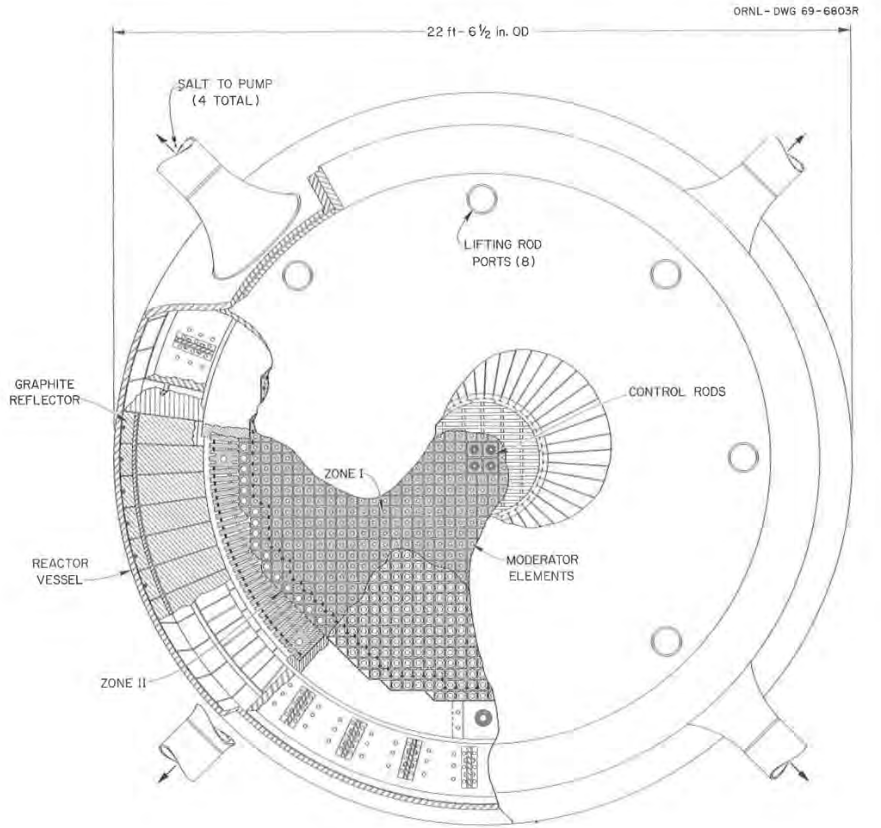
\includegraphics[width=0.5\linewidth]{figs/ch4/msbr_full_xy_ref.png}
        \label{fig:msbr-ref-xy}
    }
    \subfloat[][]{
        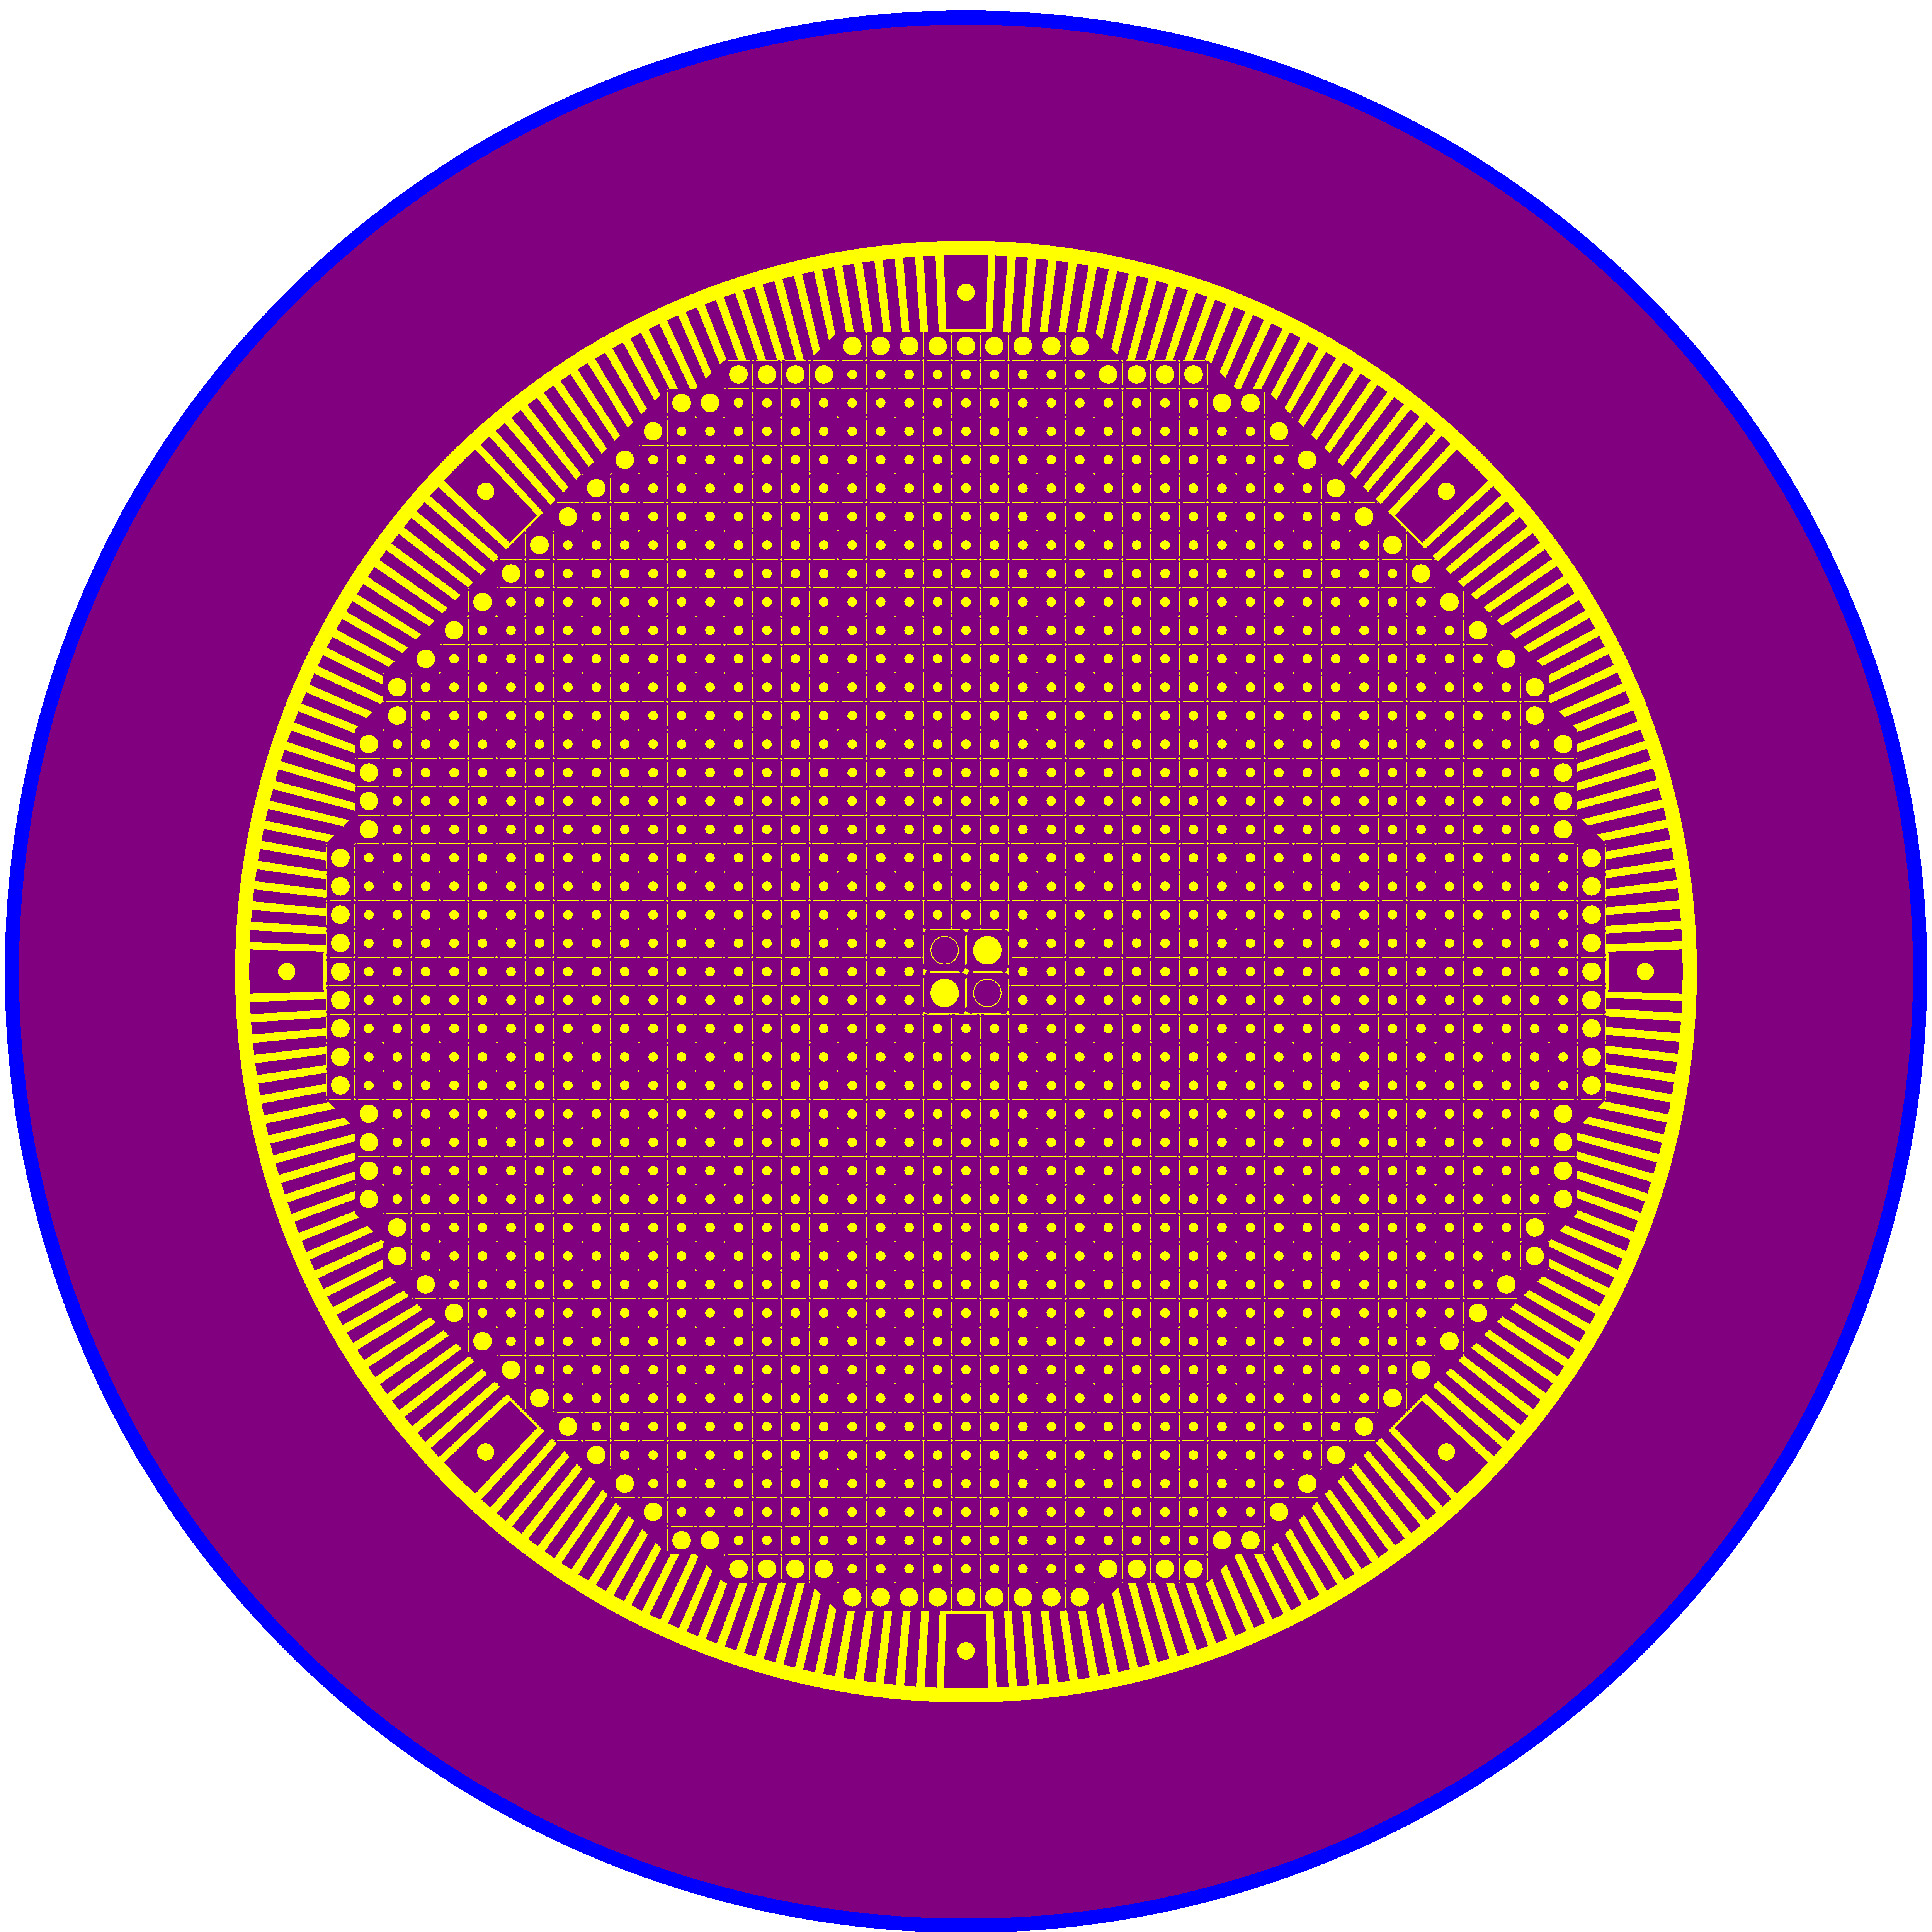
\includegraphics[width=0.5\linewidth]{figs/ch4/msbr_full_xy_openmc.png}
        \label{fig:msbr-model-xy}
    }
    \\
    \subfloat[][]{
        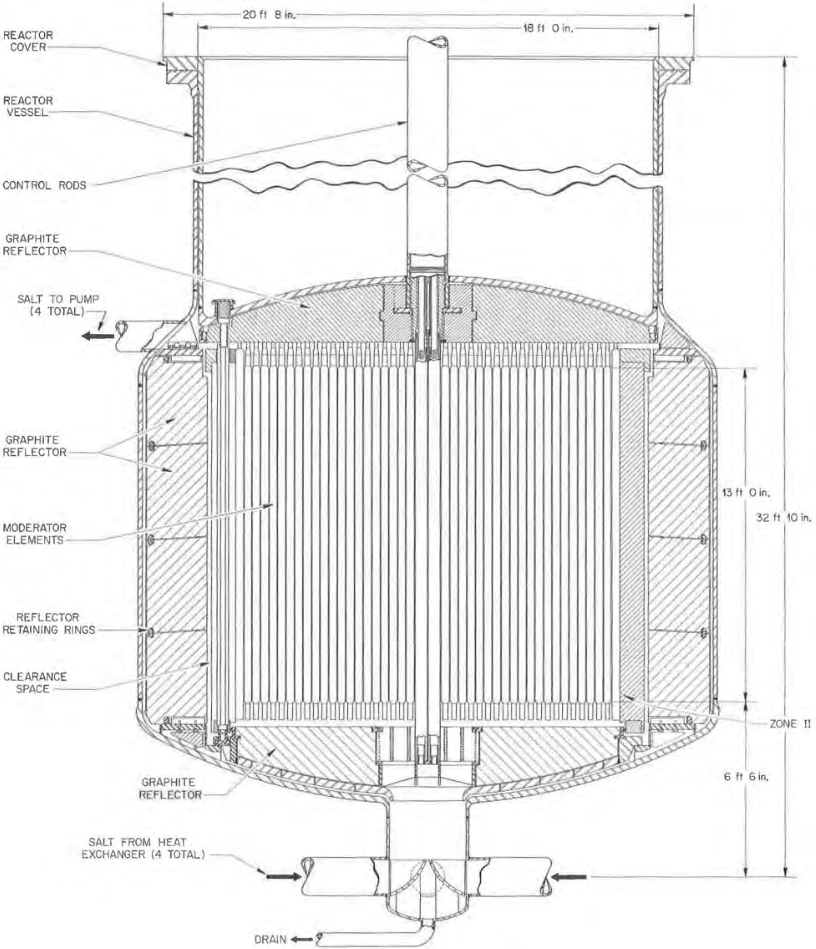
\includegraphics[width=0.5\linewidth]{figs/ch4/msbr_full_xz_ref.png}
        \label{fig:msbr-ref-xz}
    }
    \subfloat[][]{
        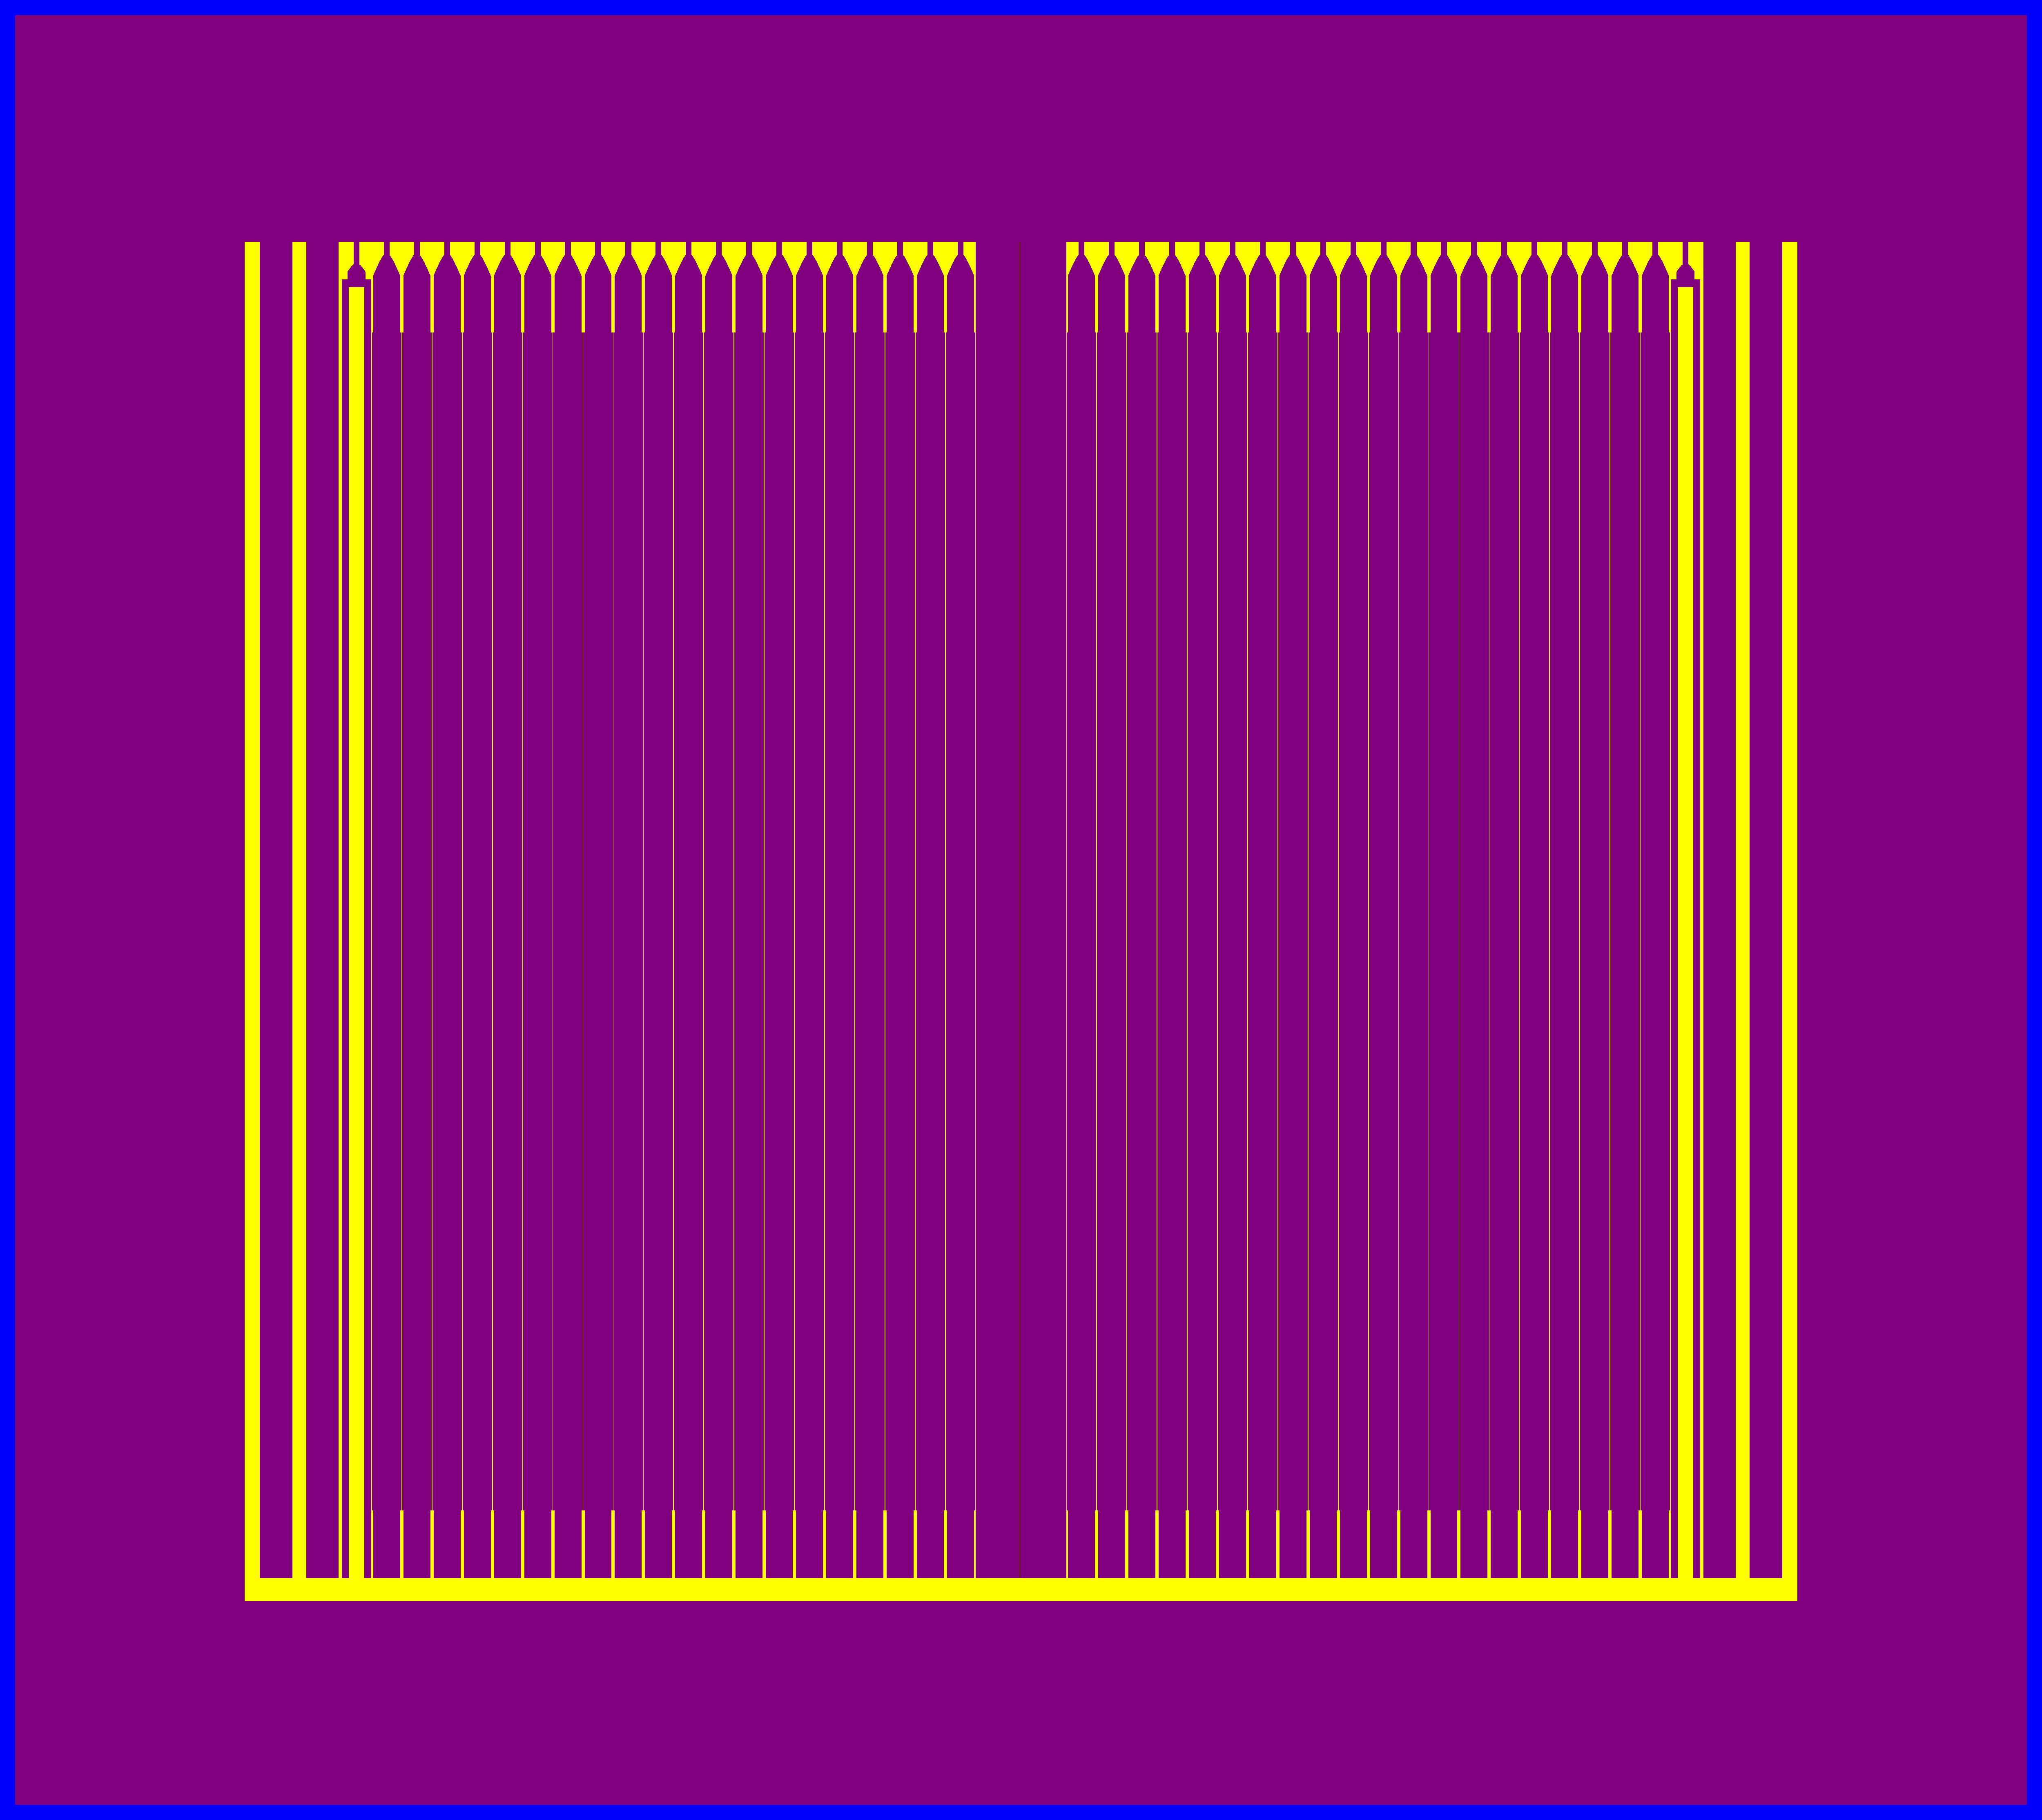
\includegraphics[width=0.5\linewidth]{figs/ch4/msbr_full_xz_openmc.png}
        \label{fig:msbr-model-xz}
    }
    \caption[Full views of MSBR]{
        \subref{fig:msbr-ref-xy} Top down view of \Gls{msbr} reference design.
        \subref{fig:msbr-model-xy} Top down view of \Gls{msbr} CSG model.
        \subref{fig:msbr-ref-xz} Side view of \Gls{msbr} reference design.
        \subref{fig:msbr-model-xz} Side view of \Gls{msbr} CSG model.
    }
    \label{fig:msbr-overview}
\end{figure}

As seen in Figure \ref{fig:msbr-overview}, the \Gls{csg} \Gls{msbr}
model reproduces these systems with several approximations. I will
describe each reactor system, as well as any relevant changes or
approximations made in the model.

\section{Materials}
\label{sec:msbr-materials}

\subsection{Fuel salt}
\label{sub:msbr-fuel-salt}
Table S.1 in Robertson et al. (1971) \cite{robertson_conceptual_1971} specifies the fuel salt
composition used in the \Gls{msbr}:
\ce{LiF}-\ce{Be}\ce{F_2}-\ce{Th}\ce{F_4}-\ce{U}\ce{F_4} at a concentration of
71.7-16-12-0.3 mole-\%. The lithium used in the fuel salt is enriched to
99.995\% \ce{^{7}Li}. This is because \ce{^{6}Li} is a strong neutron absorber
and produces tritium in the absorption reaction. The atom-\% for each nuclide is
given in Table \ref{tab:msbr-fuel-salt-ref}\footnote{Most of the discussion of
the fuel salt composition in 
\cite{robertson_conceptual_1971}
specify elemental version of the nuclides in Table \ref{tab:msbr-fuel-salt-ref}.
I have specific nuclides for the following reasons: (1) both \ce{F} and
\ce{Be} have only one stable isotope, (2) the fuel salt receives initial fissile
loading from \ce{^{233}U} or \ce{^{235}U}, and (3) the fuel salt receives its
fertile loading from \ce{^{232}Th}}\footnote{I use OpenMC's Python API with the
ENDF/V VII.0 library along with a custom Python script
(\url{github.com/arfc/2022-yardas-ms/tree/master/model/salt-composition.ipynb})
to calculate these values. You may obtain slightly different numbers if you use
a different cross section library or calculation method, but they should  be
roughly the same.}.

See Section \ref{sec:salt-volume} for additional discussion of the value used
for the salt volume\footnote{I recommend reading this section after the geometry
description in Section \ref{sec:msbr-core}}

\begin{table}[htpb] 
    \centering 
    \caption{Reference \Gls{msbr} fuel salt specifications rounded to six decimals}
    \label{tab:msbr-fuel-salt-ref}
    \begin{tabular}{|c|c|c|c|c|c|c|} 
        \hline
        & \ce{^{6}Li} & \ce{^{7}Li} & \ce{^{19}F} & \ce{^{9}Be} & \ce{^{232}Th} & \ce{^{233}U}\\
        \hline 
        atom-\% & 0.001653 & 28.349474 & 60.458679 & 6.326611 & 4.744958 & 0.118624 \\
        \hline
        mass-\% & 0.000393 & 7.851729 & 45.342587 & 2.250773 & 43.463247 & 1.091271\\ 
        \hline
    \end{tabular}
\end{table}

The density of the fuel salt is given by a function\footnote{This function 
comes from an earlier report on the Molten-Salt Reactor Program
\cite{rosenthal_molten-salt_1969}.} of temperature in \unit{\celsius} in Table
S.1 in Robertson et al. (1971) \cite{robertson_conceptual_1971}:
\begin{equation}
    \rho = 3.752 - 6.68\cdot 10^{-4} \cdot T \quad \unit{\gram\per\cubic\centi\meter}
\end{equation}

The temperature of the fuel salt flowing into the core at the inlet at the
bottom of the reactor is 1050\unit{\degree}F (565.5556\unit{\celsius}, 838.7056
\unit{\kelvin}), and the temperature of the fuel salt flowing out of the core at
the outlet is approximately 1300\unit{\degree}F (704.4444\unit{\celsius},
977.5944 \unit{\kelvin}) \cite{robertson_conceptual_1971}. The average
temperature of the salt over the core inlets and outlets is then 1175
\unit{\degree}F (635\unit{\celsius}, 908.15 \unit{\kelvin}). While the
various solid components of the core are at a slightly higher temperature on
average\footnote{see figure 3.29 in \cite{robertson_conceptual_1971}}, for
simplicity, I set the evaluated temperature of all materials to 900
\unit{\kelvin} consistent cross-section selection between the \OpenMC and
\SerpentTWO depletion steps. At this temperature, the density of the fuel salt
is 3.3332642 \unit{\gram\per\centi\metre\cubed}.

\begin{table}[htpb] 
    \centering 
    \caption{Model \Gls{msbr} fuel salt specifications rounded to six decimals}
    \label{tab:msbr-fuel-salt-model}
    \begin{tabular}{|c|c|c|c|c|c|c|} 
        \hline
        & \ce{^{6}Li} & \ce{^{7}Li} & \ce{^{19}F} & \ce{^{9}Be} & \ce{^{232}Th} & \ce{^{233}U}\\
        \hline 
        atom-\% & 0.001656 &  28.386079 & 60.435213 & 6.330366 & 4.747774 & 0.098912 \\
        \hline
        mass-\% & 0.000394 & 7.874599 & 45.398383 & 2.255756 & 43.55963 & 0.911406\\ 
        \hline
    \end{tabular}
\end{table}
% WILL NEED TO DO TEST SIMULATIONS TO CONFIRM THIS MATCHES PARK ET AL
In the CSG model, I adjusted increased the amount of \ce{Li}\ce{F} by 0.5 mol-\% and
decreased the amount of \ce{U}\ce{F_{4}} by 0.5 mol-\% for a total mol-\% composition of
71.75-16-12-0.25. When using the reference salt composition, I obtained $k_\text{eff}$
around 1.15 at \Gls{bol}, which is much too high for a power reactor. This adjustment
gives much a much more reasonable \Gls{bol} $k_{\text{eff}}$ around 1.08.
The fuel salt material uses the composition specified in Table \ref{tab:msbr-fuel-salt-model}
and has a density of 3.35 \unit{\gram\per\centi\metre\cubed}.

\subsection{Graphite}
\label{sub:graphite}

For a detailed description of the reactor graphite used in the \Gls{msbr}, see
Section 3.2.3 in Robertson et al. (1971) \cite{robertson_conceptual_1971}. At 70\unit{\degree}F (294.3
\unit{\kelvin}), the \Gls{msbr} graphite has a density of 1843
\unit{\kilo\gram\per\cubic\metre}. This is the only density specification
for graphite that I was able to find in Robertson et al. (1971)
\cite{robertson_conceptual_1971}. In the CSG model, the graphite material uses
elemental carbon and has a density of 1.84 \unit{\gram\per\centi\metre\cubed}.

\subsection{Modified Hastelloy N}
\label{sub:hastelloy}
Hastelloy N is an alloy developed at \Gls{ornl} during the Molten-Salt Reactor
Program. It was developed as a material that could maintain structural stability while
in contact with the corrosive and high temperature molten salt fuel while also
being under irradiation for a long period of time.

The \Gls{msbr} used a modified version of Hastelloy N designed to improve
embrittlement resistance and weldability \cite{robertson_conceptual_1971}.
The \Gls{msbr} uses modified Hastelloy N on all nearly all salt-facing
components included in the CSG model.

Modified Hastelloy N has a density of 8671 \unit{\kilo\gram\per\cubic\metre} at
1300\unit{\degree}F (704.4444\unit{\celsius}, 977.5944 \unit{\kelvin})
\cite{robertson_conceptual_1971}. The elemental composition of modified
Hastelloy N and their amounts in mass-\% are in Table \ref{tab:hastelloy-n-ref}.

\begin{table}[htpb]
    \centering
    \caption[Mass-\% of elements in modified Hastelloy N used in the \Gls{msbr}]{Mass-\% of elements in modified Hastelloy N used in the \Gls{msbr}. Data from Table 3.1 and S.1 in \cite{robertson_conceptual_1971}. Ranged values collapsed to their average are denoted with a $^*$}
    \label{tab:hastelloy-n-ref}
    \begin{tabular}{|c|c|c|c|c|c|c|c|c|c|c|c|c|c|c|c|c|}
        \hline
        \ce{Ni} & \ce{Mo}$^*$ & \ce{Cr}$^*$ & \ce{Fe}$^*$ & \ce{C}$^*$ & \ce{Mn}$^*$ & \ce{Si} & \ce{W} & \ce{Al} & \ce{Ti}$^*$ & \ce{Cu} & \ce{Co} & \ce{P} & \ce{S} & \ce{B} & \ce{Hf}$^*$ & \ce{Nb}$^*$ \\
        \hline
        73.709 & 12 & 7 & 3 & 0.06 & 0.35 & 0.1 & 0.1 & 0.1 & 1.25 & 0.1 & 0.2 & 0.015 & 0.015 & 0.001 & 1 & 1\\
        %\hline
        %atom-\% & 76.72 & 7.64 & 8.224 & 3.282 & 0.305 & 0.389 & 0.218 & 0.033 & 0.226 & 1.595 & 0.096 & 0.207 & 0.03 & 0.029 & 0.006 & 0.342 & 0.658 \\
        \hline
    \end{tabular}
\end{table}

The Hastelloy N material in the CSG model uses the composition specified in
Table \ref{tab:hastelloy-n-ref} and has a density of 8.671 
\unit{\gram\per\centi\metre\cubed}.


\section{Reactor core}
\label{sec:msbr-core}
The \Gls{msbr} core is split into three distinct different zones: zone I, zone
II, and the reflector zone. 

\begin{figure}[htpb]
    \centering
    \subfloat[][]{
        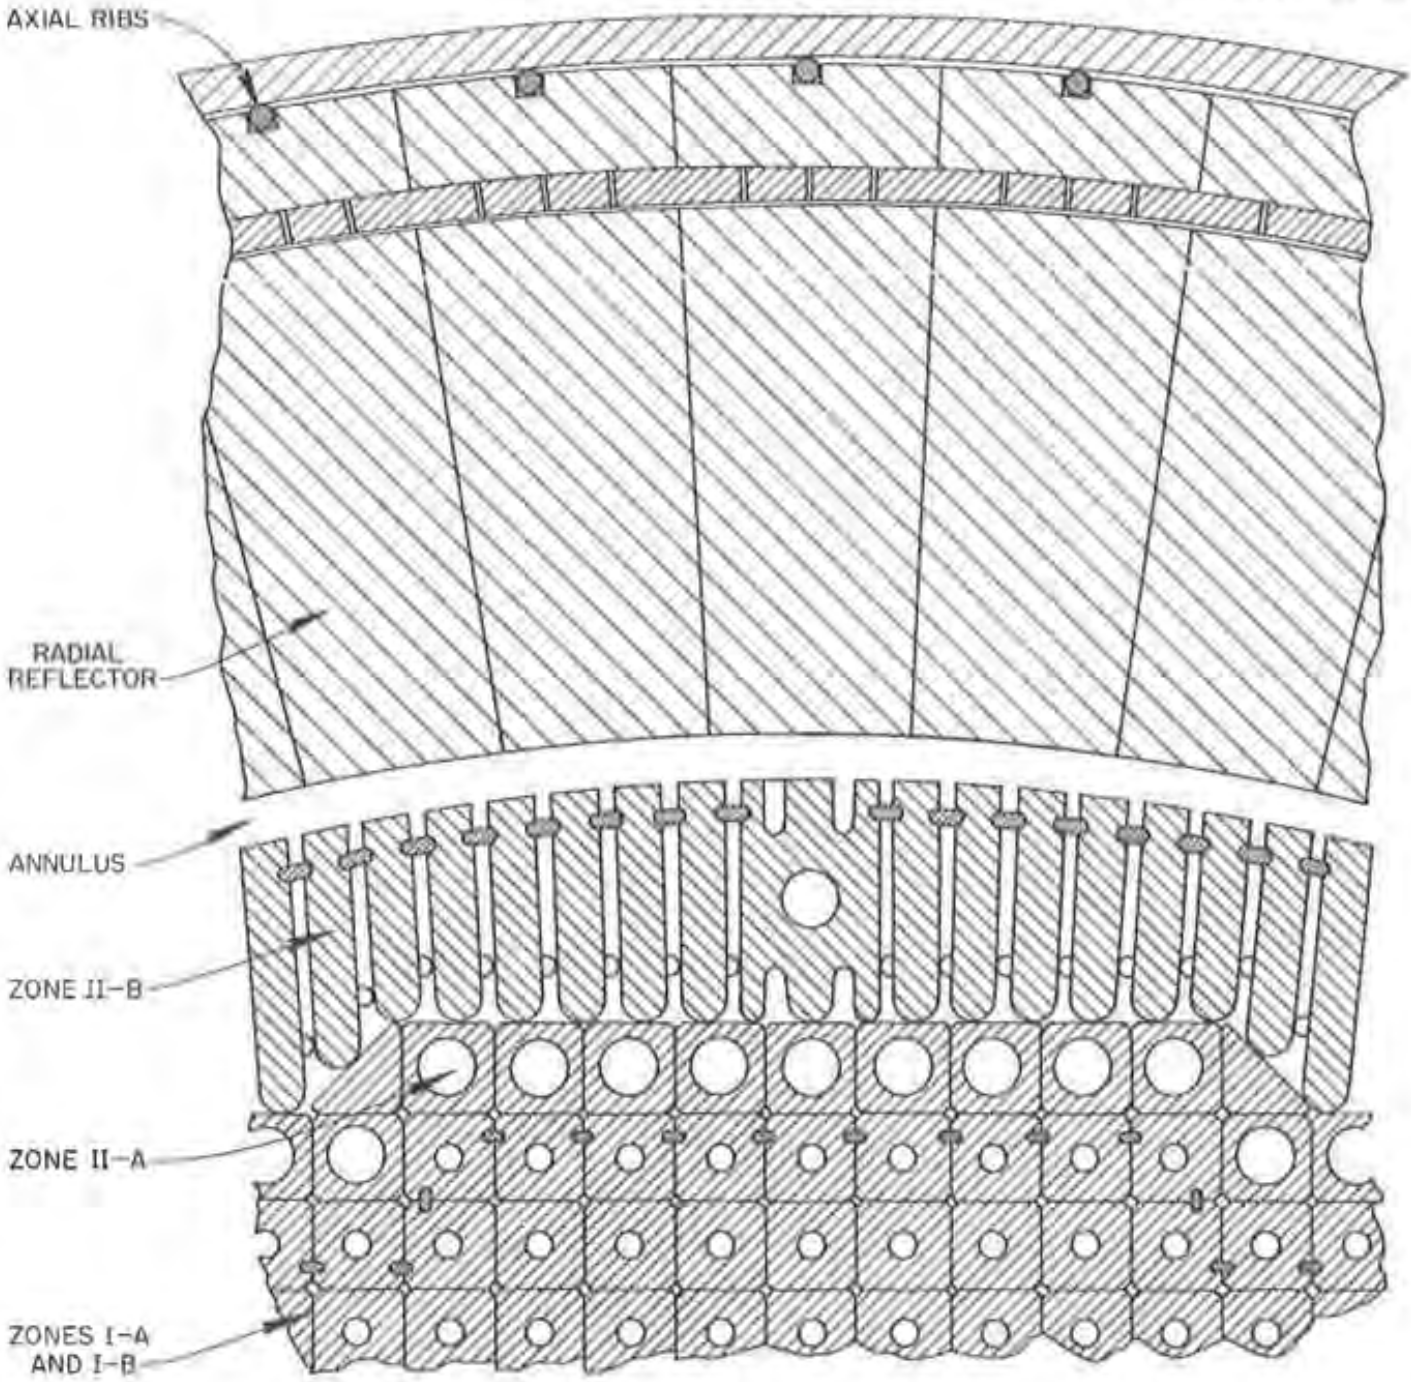
\includegraphics[width=0.45\linewidth]{figs/ch4/msbr_section_ref.png}
        \label{fig:msbr_sec_ref}
    }
    \subfloat[][]{
        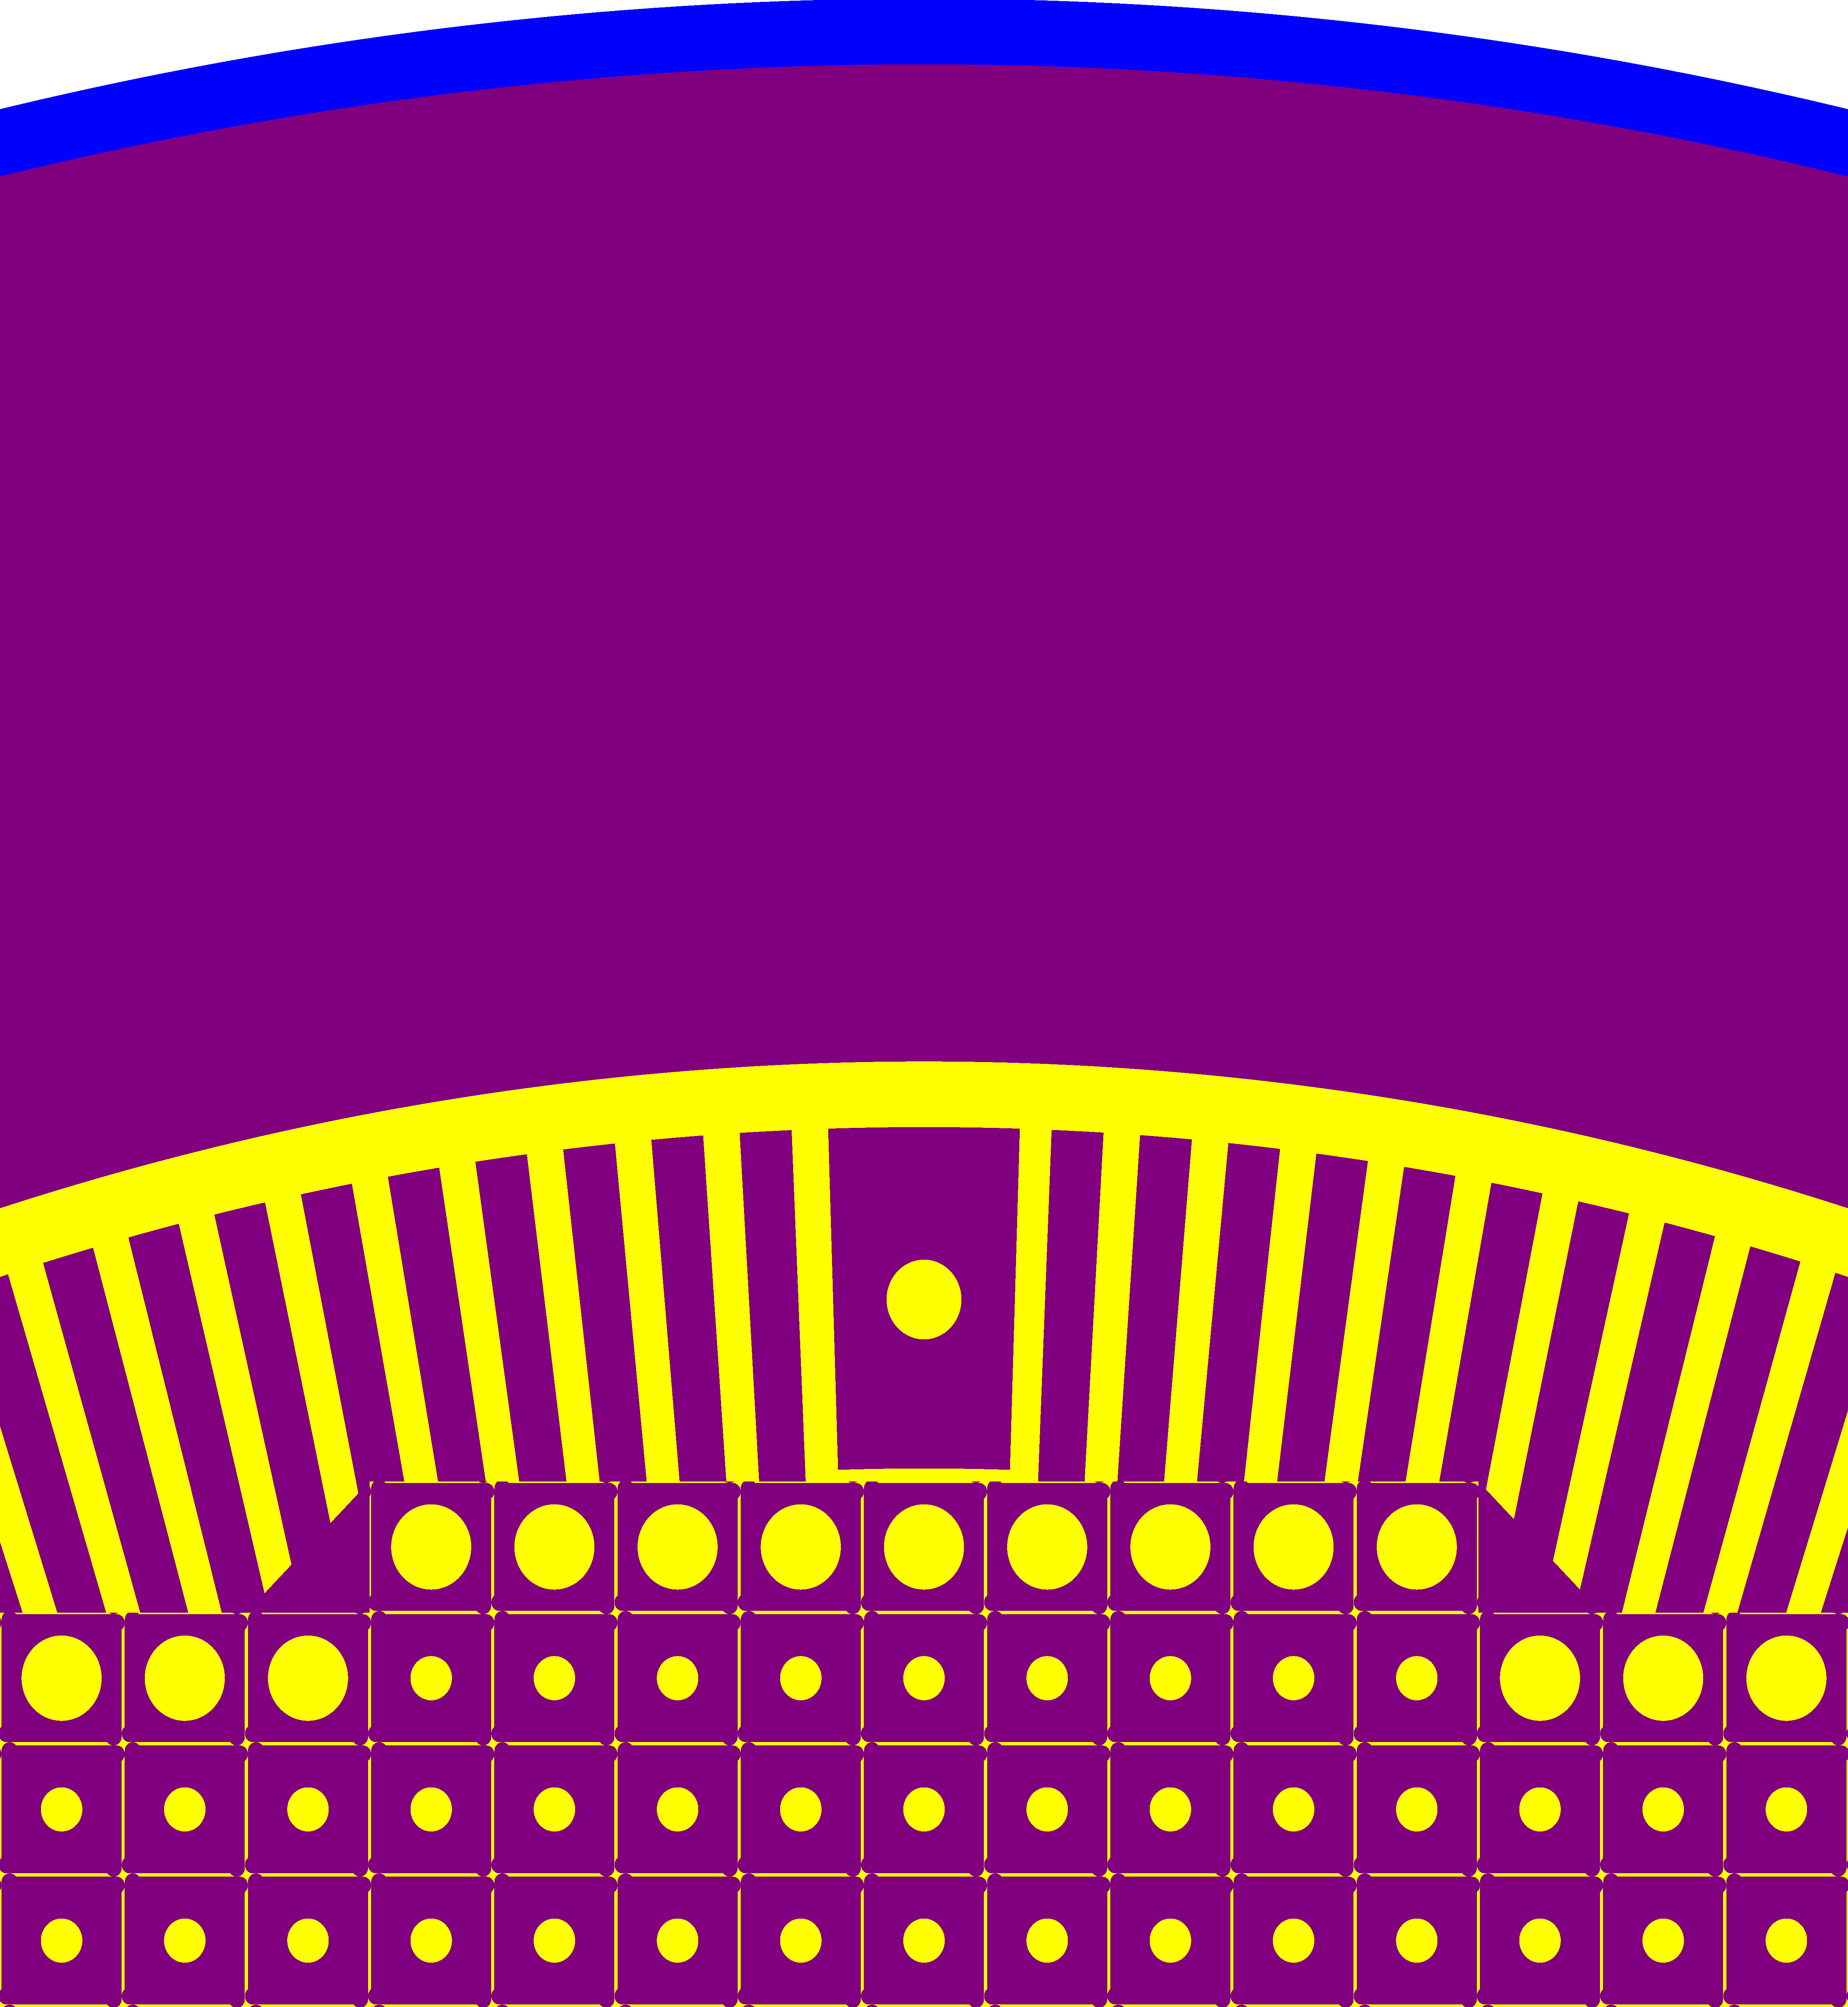
\includegraphics[width=0.35\linewidth]{figs/ch4/msbr_section_openmc.png}
        \label{fig:msbr_sec_model}
    }
    \caption[Detail views of MSBR core region]{
        \subref{fig:msbr_sec_ref} Detail view of \Gls{msbr} reference design.
        \subref{fig:msbr_sec_model} Detail view of \Gls{msbr} CSG model.}
    \label{fig:msbr-detail}
\end{figure}

\subsection{Zone I} Zone I is the central-most region of the core, and is 13.2\%
fuel salt by volume. Zone I is divided into three subzones: zone I-A, zone I-B,
and the control rod zone.

Zone I-A and I-B consist of 4 in. $\times$ 4 in. (10.16 cm $\times$ 10.16 cm)
square graphite elements. As seen in Figures \ref{fig:msbr-ia-xy} and
\ref{fig:msbr-ib-xy}, elements in both zones have axial ribs protruding from
the faces of the square elements near the corners, as well as cylindrical
channels in the centers of the elements. The purpose of the fuel holes are to
facilitate salt flow through the core elements. The purpose of the ribs are to
separate the elements from each other as well as create interstitial salt flow
channels \cite{robertson_conceptual_1971}. These interstitial flow channels
are seen in Figures \ref{fig:msbr-ia-lattice} and
\ref{fig:msbr-ib-lattice}\footnote{Notice that the shape of the model zone I-B
elements qualitatively matches the reference design in Figure
\ref{fig:msbr-ib-xy}, but  not in Figure \ref{fig:msbr-ib-lattice}, despite
matching nearly all specifications of the reference design.}.

The only dimensional differences between the zone I-A and I-B elements are the
diameter of the cylindrical fuel channels and the size of the axial ribs (see
Tables \ref{tab:zone-ia-ref-specs} and \ref{tab:zone-ib-specs}). Zone I-A
elements have a smaller cylindrical channel and larger interstitial channel
than zone I-B elements. The central part of zone I consists of zone I-A
elements, whereas the outer part of zone I consists of zone I-B
elements \cite{robertson_conceptual_1971}. The purpose this configuration is to
reduce the temperature gradient across the core. The salt velocity through the
zone I-B elemets is much lower than the salt velocity through the zone I-A
elements\footnote{Robetson et al. (1971) states that the salt velocity varies
``from 8 fps at the center [of the core] to about 2 fps near the periphery''
\cite{robertson_conceptual_1971}}.

Additionally the zone I elements are machined to a cylindrical shape at the ends
to create an undermoderated region of 37\% salt at the top and bottom of the
reactor \cite{robertson_conceptual_1971}. These machined ends are referred to as
Section A (see Figures \ref{fig:msbr-ia-xy}, \ref{fig:msbr-ib-xy}, and
\ref{fig:msbr-i-xz-full}). The top of each element also has an outlet plenum to
direct salt flow towards the exit nozzles at the edge of the vessel, however
these are not included in the \Gls{csg} model. The outermost layer of zone I
elements also have grooves in them to fit eliptical graphite sealing rods (see
Figure \ref{fig:msbr-detail}) that separate the salt flow in zone I from the
salt flow in zone II \cite{robertson_conceptual_1971}. Robertson et al. (1971)
does not specify precise dimensions and positions of these rods, so they are not
included in the \Gls{csg} model.

Robertson et al. (1971) does not specify exact distribution of zone I-A and I-B
elements. Rather than guess the distribution of I-A and I-B elements, the CSG
model assumes that zone I consists entirely of I-B elements. This assumption
greatly simplifies the work needed to create the model. Had we picked zone I-A
elements, we would have needed to create at least eight different ``versions''
of both the I-A elements and the II-A elements\footnote{four versions of each
element for each configuration where a I-A and II-A element are adjacent,
four versions of I-A elements for each configuration where the element is
adjacent to two II-A elements, and four versions of II-A elements for each for
configuration where the II-A element is adjacent to two I-A elements.}

\begin{table}[htpb]
    \centering
    \caption{Reference Zone I-A dimensions}
    \label{tab:zone-ia-ref-specs}
    \begin{tabulary}{\linewidth}{|C|C|C|}
    \hline
    Quantity & Dimension [in] & Dimension [\unit{\centi\metre}]\\
    \hline
    Section A inner diameter & 0.6 & 1.524 \\
    \hline
    Section A outer diameter & 3.698 & 9.39292 \\
    \hline
    Rib tip radius of curvature & 0.25 & 0.635 \\
    \hline
    Rib tip to element spacing & 0.302 & 0.76708 \\
    \hline
    Rib tip to element center & 1.315 & 3.3401 \\
    \hline
    Zone A height (bottom) & 9 & 22.86\\
    \hline
    Zone B height & 156 & 396.24 \\
    \hline
    Zone A height (top) & 7.5 & 19.05 \\
    \hline
    Conical part height & 2.75 & 6.985 \\
    \hline
    Hastelloy plug height & 2.875 & 7.3025 \\
    \hline
    Hastelloy plug diameter & 0.6 & 1.524 \\
    \hline
    Top part height & 1.75 & 4.445 \\
    \hline
    Top part outer diameter & 1.75 & 4.445 \\
    \hline
    \end{tabulary}
\end{table}


\begin{table}[htpb]
    \centering
    \caption{Zone I-B dimensions}
    \label{tab:zone-ib-specs}
    \begin{tabulary}{\linewidth}{|C|CC|CC|}
    \hline
    Quantity & Reference Dimension [in] & Reference Dimension [\unit{\centi\metre}] & Model Dimension [in] & Model Dimension [\unit{\centi\metre}]\\
    \hline
    Section A inner diameter & 1.340 (Fig. \ref{fig:msbr_ib_bottom_ref}) or 1.347 (Fig. \ref{fig:msbr_ib_lattice_ref}) & 3.4036 or 3.42138 & 1.347 & 3.42138 \\
    \hline
    Section A outer diameter & 3.900 & 9.906 & 3.900 & 9.906 \\
    \hline
    Rib tip radius of curvature & 0.25 & 0.635 & 0.263 & 0.66802\\
    \hline
    Rib tip to element spacing & 0.1 & 0.254 & 0.1 & 0.254\\
    \hline
    Rib tip to element center & 1.687 & 4.28498 & 1.687 & 4.28498\\
    \hline
    Zone A height (bottom) & 9 & 22.86 & 9 & 22.86\\
    \hline
    Zone B height & 156 & 396.24 & 156 & 396.24\\
    \hline
    Zone A height (top) & 7.5 & 19.05 & 7.5 & 19.05\\
    \hline
    Conical part height & 2.75 & 6.985 & 2.75 & 6.985\\
    \hline
    Hastelloy plug height & 2.875 & 7.3025 & 1.75 & 4.445 \\
    \hline
    Hastelloy plug diameter & 1.340 (Fig. \ref{fig:msbr_ib_bottom_ref}) or 1.347 (Fig. \ref{fig:msbr_ib_lattice_ref}) & 3.4036 or 3.42138 & 1.347 & 3.42138 \\
    \hline
    Top part height & 1.75 & 4.445 & 1.75 & 4.445 \\
    \hline
    Top part outer diameter & 1.75 & 4.445 & 1.75 & 4.445\\
    \hline
    \end{tabulary}
\end{table}


\begin{figure}[htpb]
    \centering
    \subfloat[][]{
        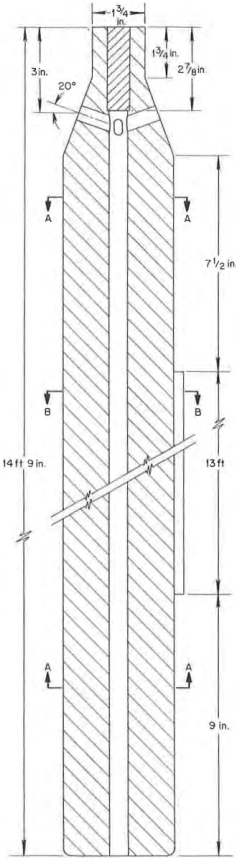
\includegraphics[width=0.25\linewidth]{figs/ch4/zone_i_full_ref.png}
        \label{fig:msbr_i_full_ref}
    }
    \subfloat[][]{
        
\includegraphics[width=0.17\linewidth]{figs/ch4/zone_ib_full_openmc.png}
        \label{fig:msbr_ib_full_model}
    }
    %\end{tabular}
    \caption[$xz$ cross sections of Zone I elements]{
        \subref{fig:msbr_i_full_ref} Reference zone I element
        \subref{fig:msbr_ib_full_model} Model zone I-B element
    }
    \label{fig:msbr-i-xz-full}
\end{figure}

\begin{figure}[htpb]
    \centering
    \subfloat[][]{
        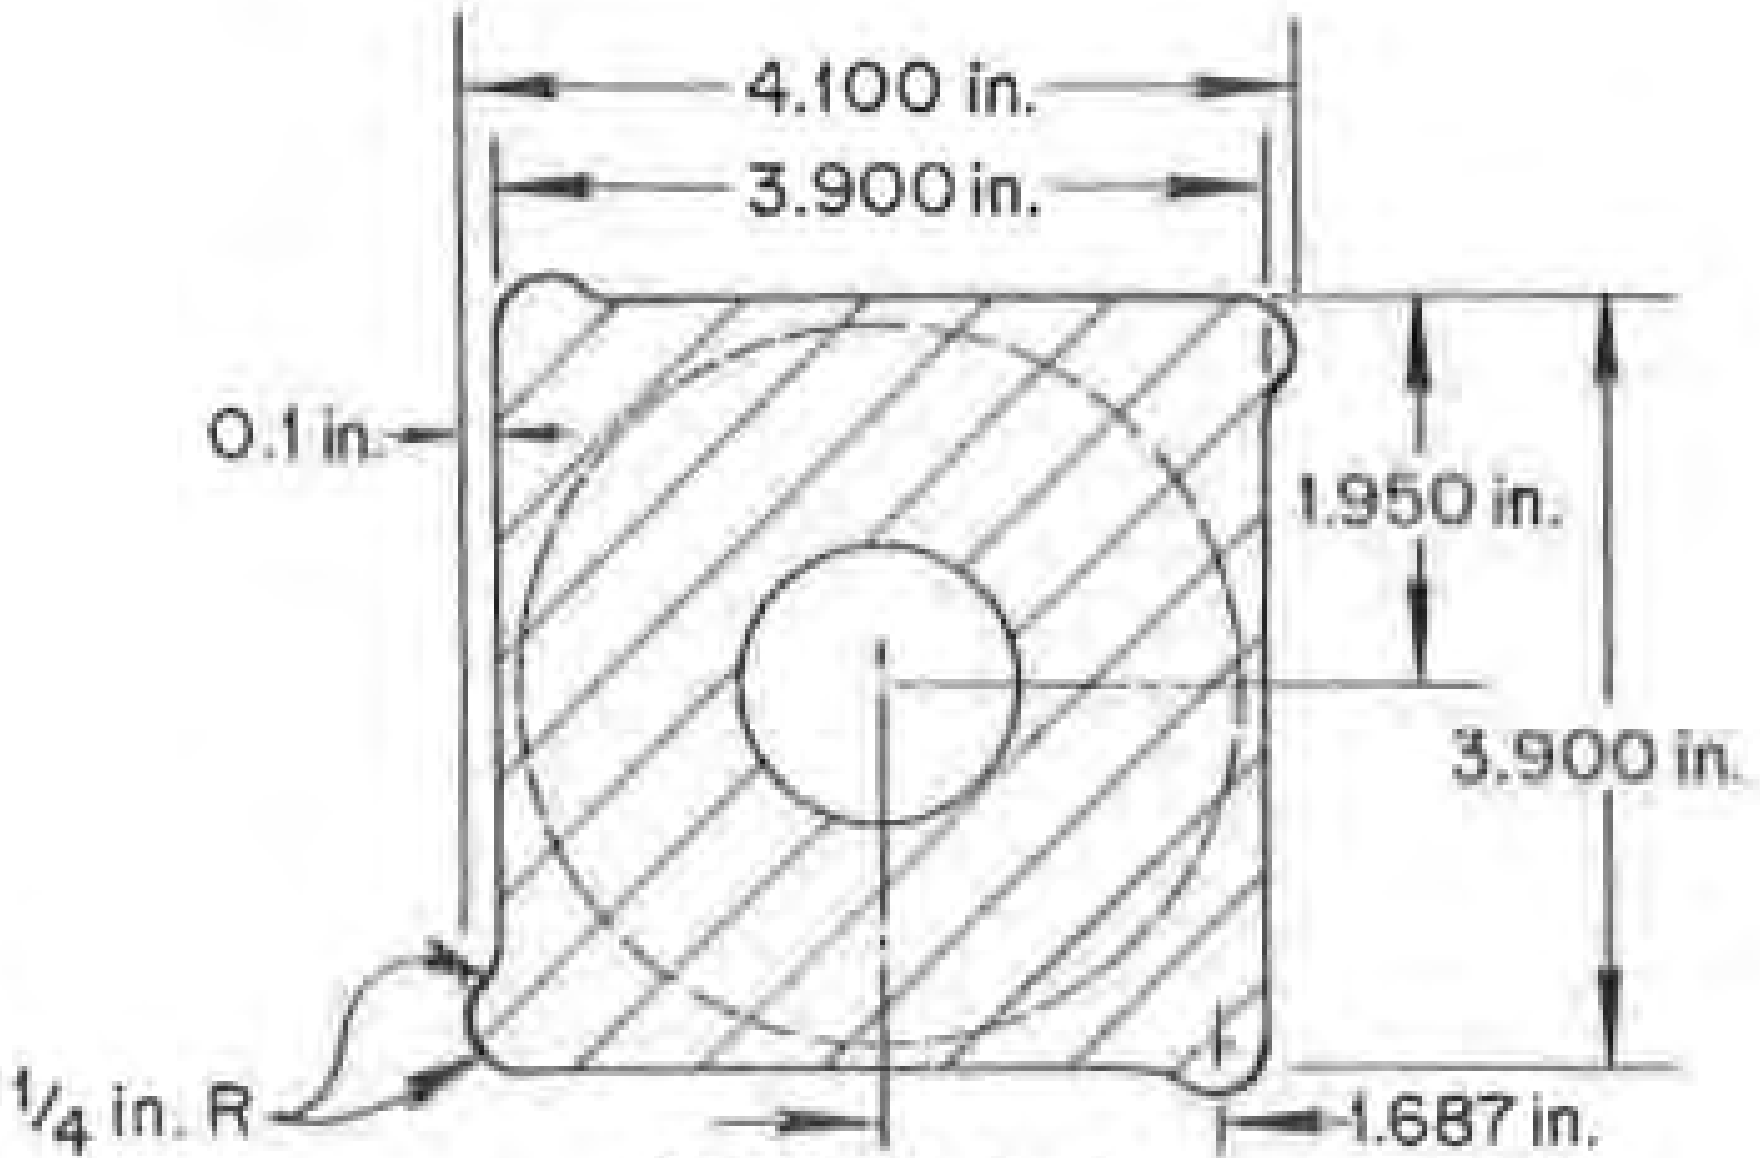
\includegraphics[width=0.3\linewidth]{figs/ch4/zone_ib_main_ref.png}
        \label{fig:msbr_ib_main_ref}
    }
    \subfloat[][]{
        
\includegraphics[width=0.2\linewidth]{figs/ch4/zone_ib_main_openmc.png}
        \label{fig:msbr_ib_main_model}
    }
    \\
    \subfloat[][]{
        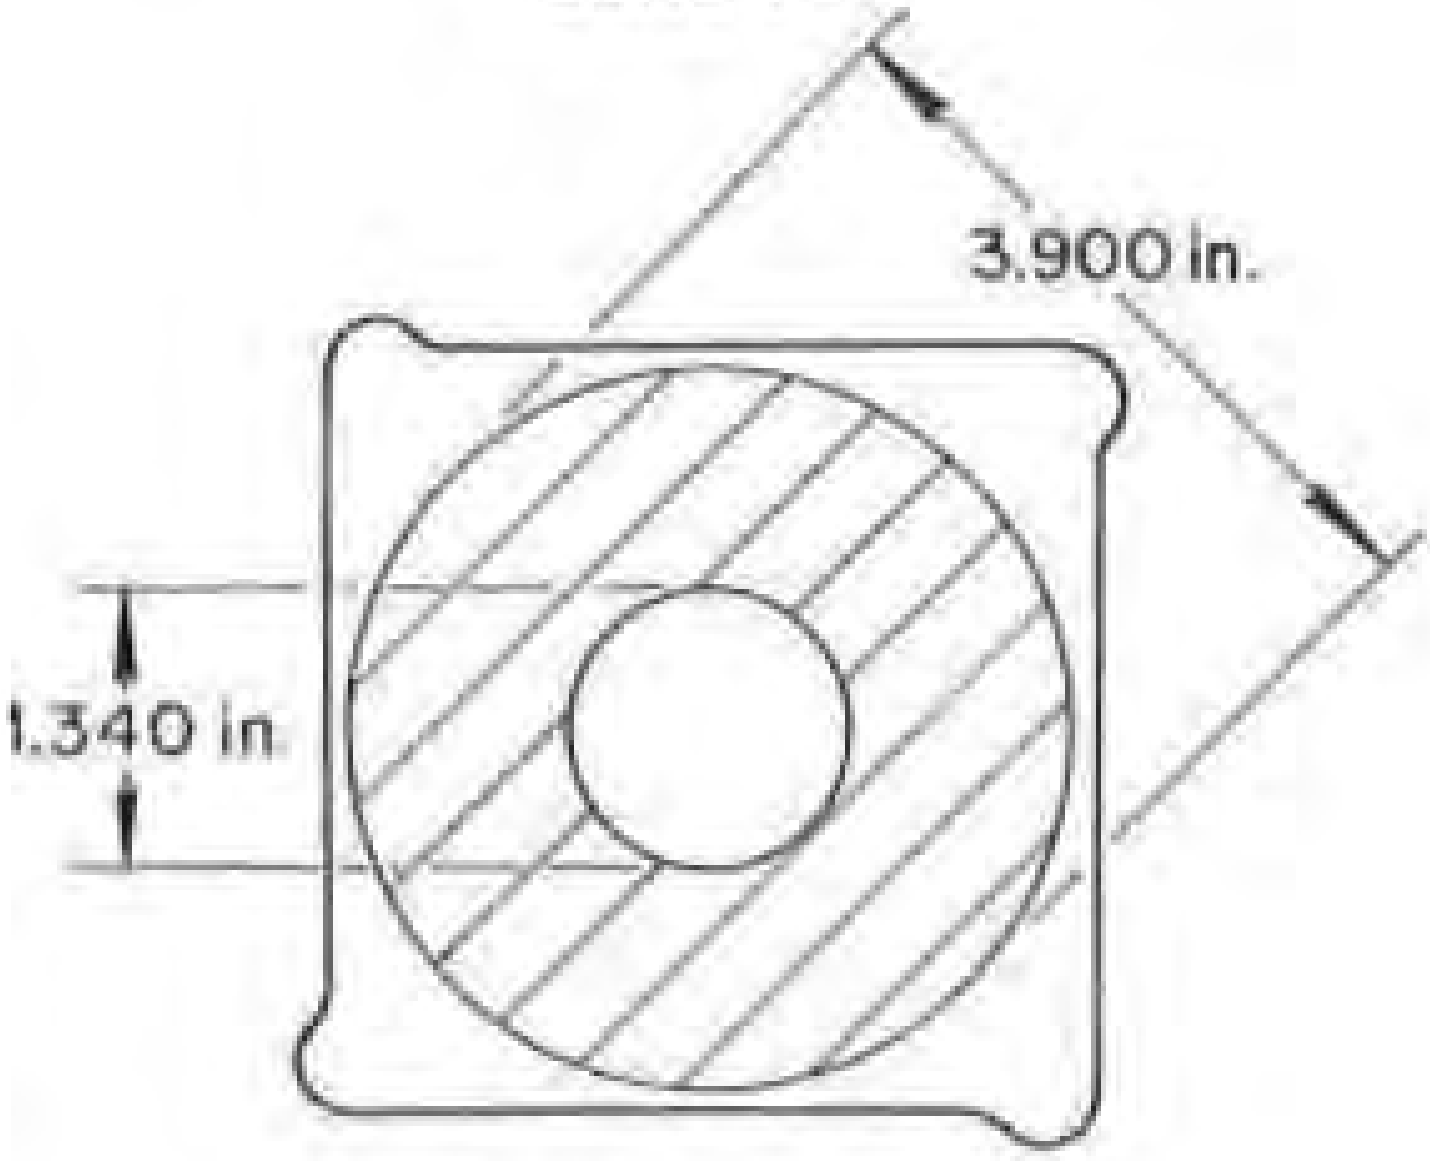
\includegraphics[width=0.3\linewidth]{figs/ch4/zone_ib_bottom_ref.png}
        \label{fig:msbr_ib_bottom_ref}
    }
    \subfloat[][]{
        
\includegraphics[width=0.2\linewidth]{figs/ch4/zone_ib_bottom_openmc.png}
        \label{fig:msbr_ib_bottom_model}
    }
    \caption[$xy$ cross sections of Zone I-B elements]{
        \subref{fig:msbr_ib_main_ref} Reference zone I-B element; section B.
        \subref{fig:msbr_ib_main_model} Model zone I-B element; section B.
        \subref{fig:msbr_ib_bottom_ref} Reference zone I-B element; section A.
        \subref{fig:msbr_ib_bottom_model} Model zone I-B element; section A.
    }
    \label{fig:msbr-ib-xy}
\end{figure}

\begin{figure}[htpb]
    \centering
    \subfloat[][]{
        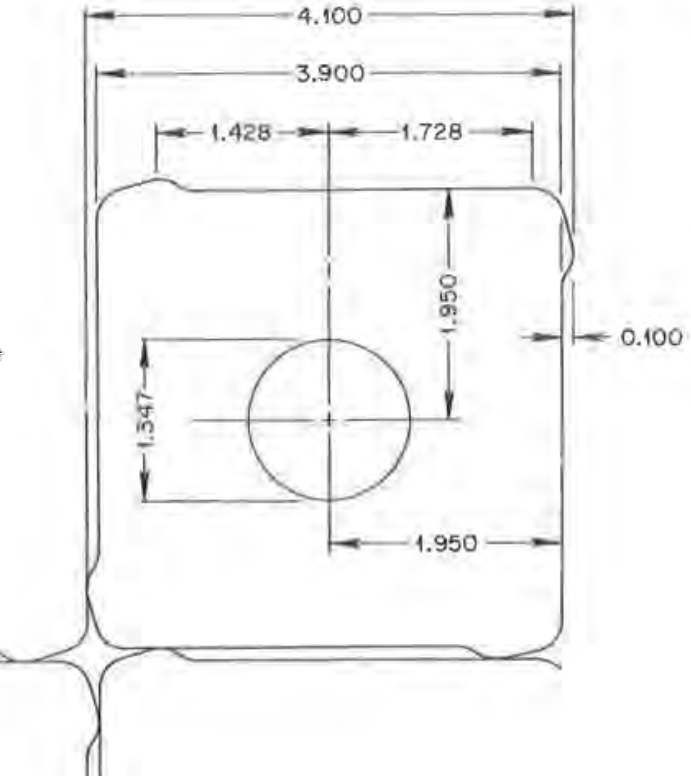
\includegraphics[width=0.25\linewidth]{figs/ch4/zone_ib_lattice_ref.png}
        \label{fig:msbr_ib_lattice_ref}
    }
    \subfloat[][]{
        
\includegraphics[width=0.17\linewidth]{figs/ch4/zone_ib_lattice_openmc.png}
        \label{fig:msbr_ib_lattice_model}
    }
    %\end{tabular}
    \caption[Lattice view of Zone I-B elements]{
        \subref{fig:msbr_ib_lattice_ref} Reference zone I-B lattice
        \subref{fig:msbr_ib_lattice_model} Model zone I-B lattice 
    }
    \label{fig:msbr-ib-lattice}
\end{figure}


\begin{figure}[htpb]
    \centering
    \subfloat[][]{
        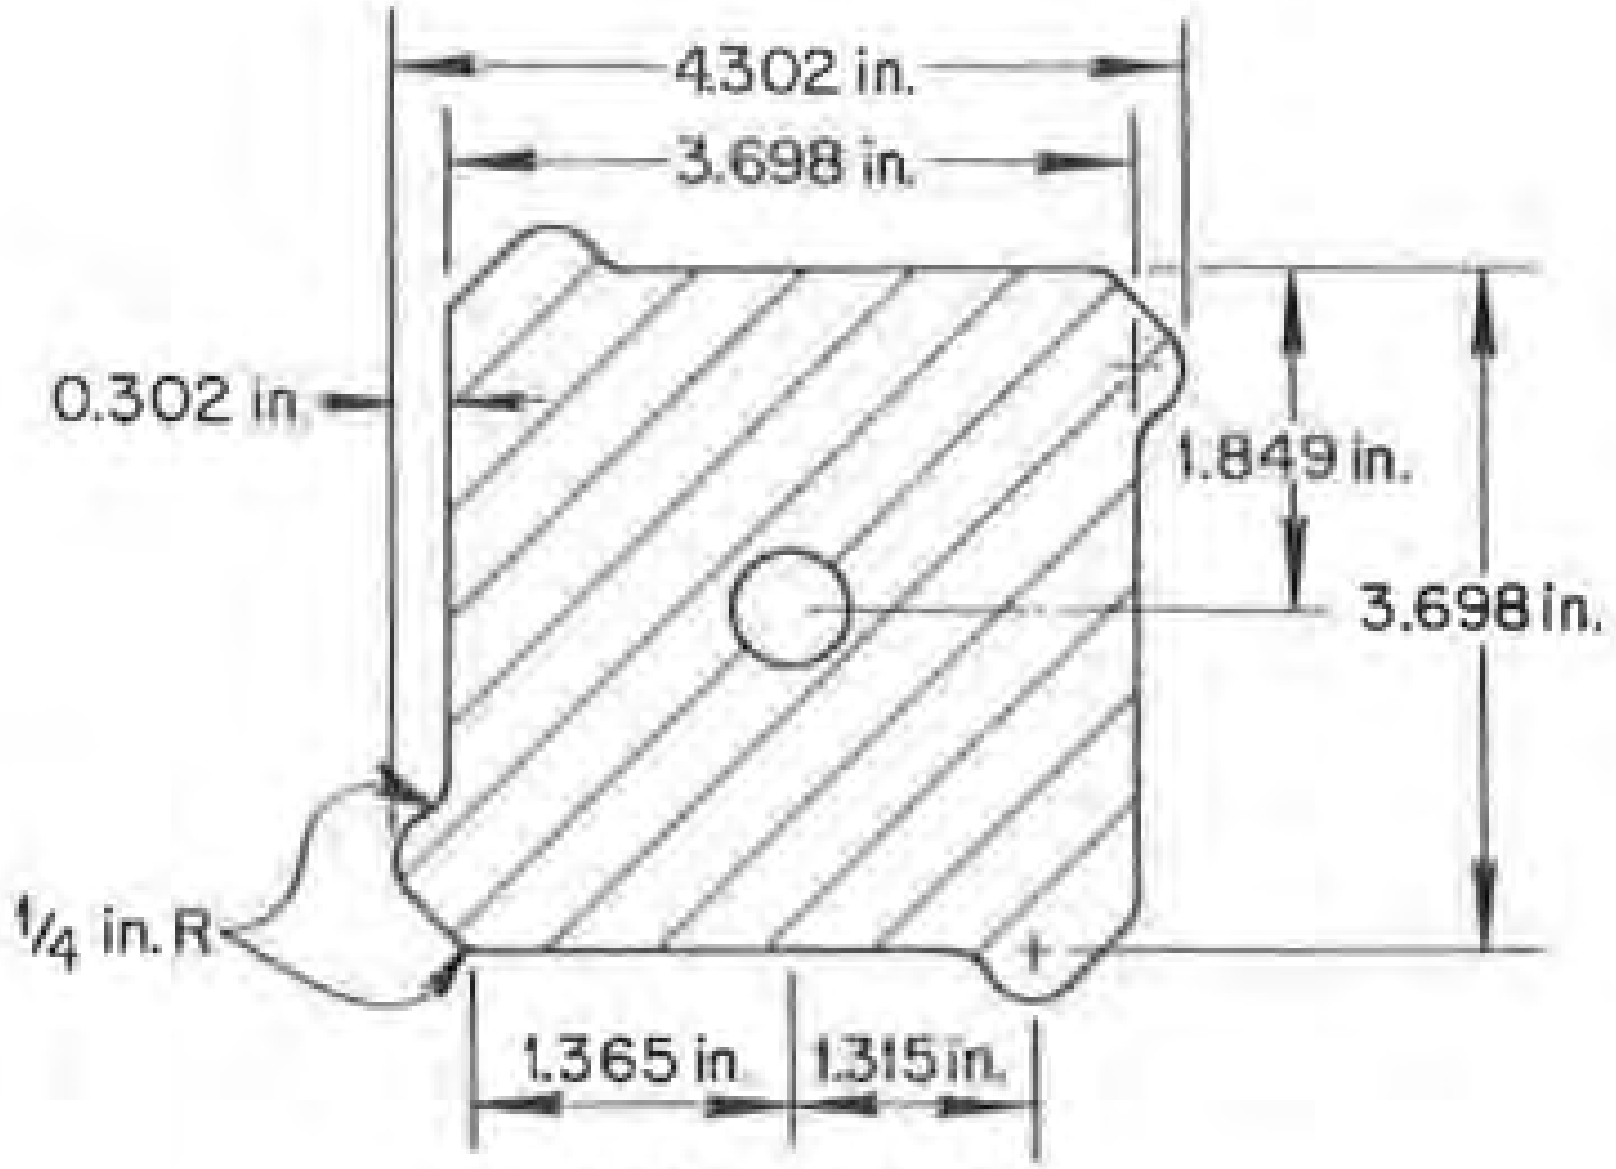
\includegraphics[width=0.3\linewidth]{figs/ch4/zone_ia_main_ref.png}
        \label{fig:msbr_ia_main_ref}
    }
    \subfloat[][]{
        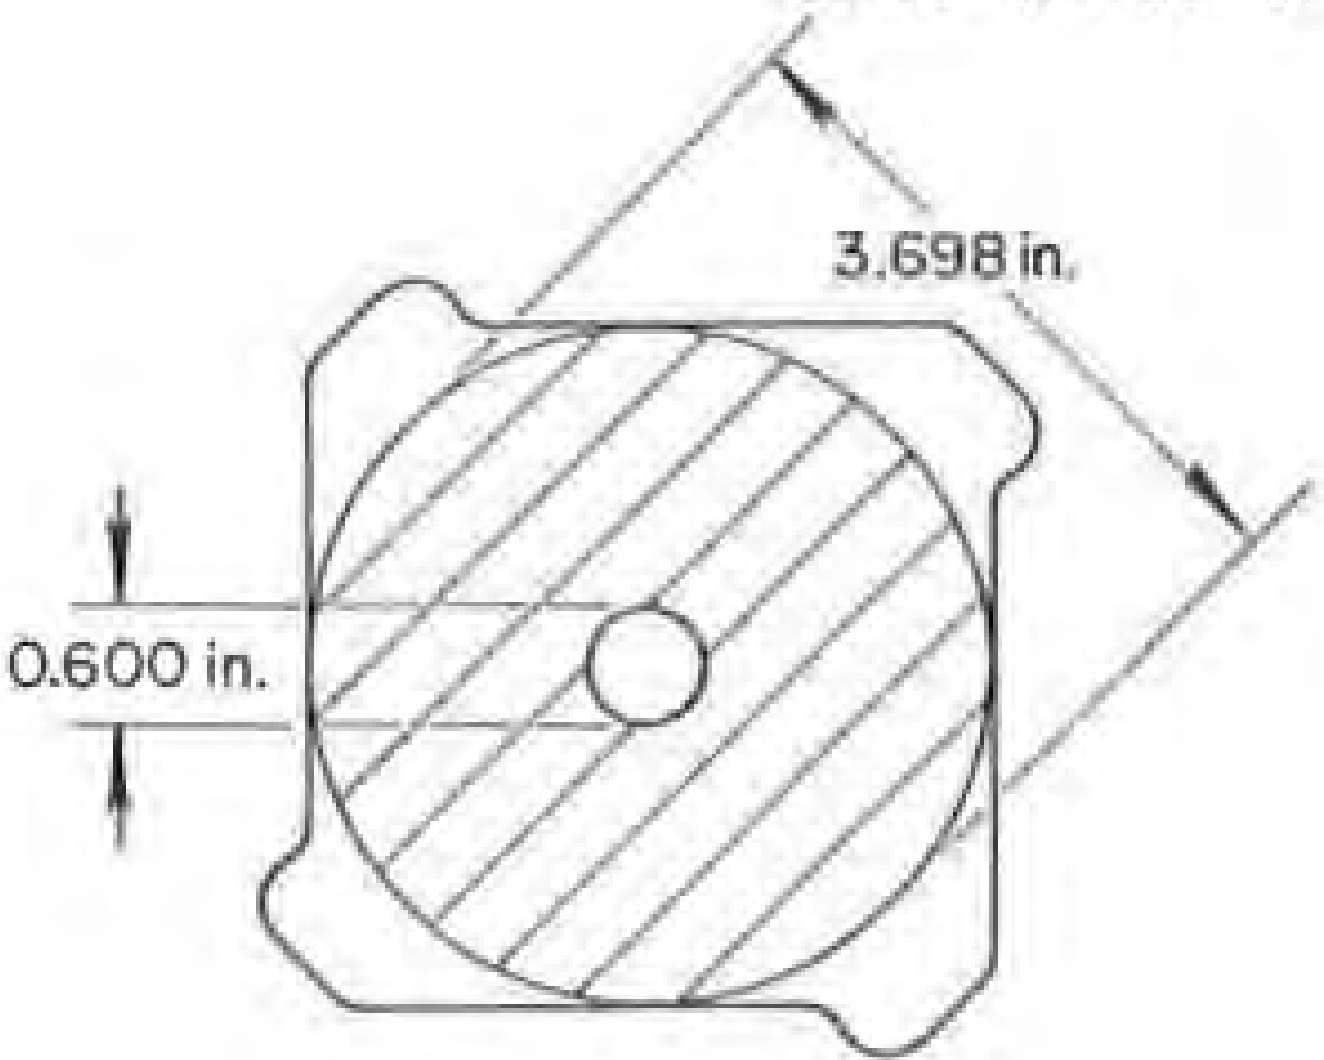
\includegraphics[width=0.3\linewidth]{figs/ch4/zone_ia_bottom_ref.png}
        \label{fig:msbr_ia_bottom_ref}
    }
    \caption[$xy$ cross sections of Zone I-A elements]{
        \subref{fig:msbr_ia_main_ref} Reference zone I-A element; Section B.
        \subref{fig:msbr_ia_bottom_ref} Reference zone I-A element; Section A.
    }
    \label{fig:msbr-ia-xy}
\end{figure}

\begin{figure}[htpb]
    \centering
    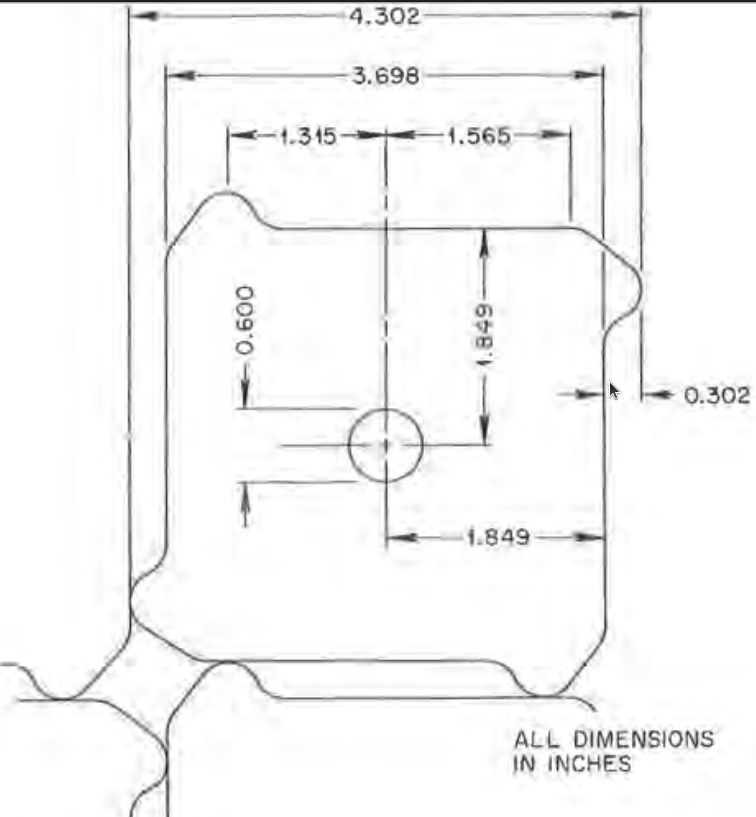
\includegraphics[width=0.25\linewidth]{figs/ch4/zone_ia_lattice_ref.png}
    \caption{Lattice view of zone I-A elements}
    \label{fig:msbr-ia-lattice}
\end{figure}

Four 6 in. $\times$ 6 in.
(15.24-cm $\times$ 15.24-cm) graphite elements
sit at the center of the core. Two of these elements contain graphite control
rods, and the other two elements are for neutron-absorbing rods for shutting
down the reactor, and are left empty during operation
\cite{robertson_conceptual_1971}. Robertson el al does not specify a design nor
dimensions for the control rod graphite elements. The \Gls{csg} model assumes
that these elements will be similar in shape to the zone I-A element (see Table
\ref{tab:cr-specification} and Figure \ref{fig:control-rods}). The control rods
themselves have axial passages through them to facilitate salt flow, but the
dimensions of these passages are not given, so the \Gls{csg} model does not
include them.

\begin{table}[htpb]
    \centering
    \caption{Control rod specifications}
    \label{tab:cr-specification}
    \begin{tabulary}{\linewidth}{|C|CC|CC|}
        \hline
        Quantity & Reference Dimension [in] & Reference Dimension [\unit{\centi\metre}] & Model Dimension [in] & Model Dimension [\unit{\centi\metre}]\\
        \hline
        Control rod element side length & 6 & 15.24 & 5.698 & 14.47292 \\
        \hline
        Control rod element inner diameter & 4 & 10.16 & 4 & 10.16\\
        \hline
        Control rod diameter & 3.75 & 9.525 & 3.75 & 9.525 \\
        \hline
        Rib tip radius of curvature & -  & - & 0.3897638 & 0.99\\
        \hline
        Rib tip to element spacing & - & - & 0.302 & 0.76708 \\
        \hline
        Rib tip to element center & - & - & 3.151 & 8.00354\\
        \hline
    \end{tabulary}
\end{table}

\begin{figure}[htpb]
    \centering
    
\includegraphics[width=0.5\textwidth]{figs/ch4/cr_xy_openmc.png}
    \caption{CSG model control rod lattice}
    \label{fig:control-rods}
\end{figure}


\subsection{Zone II}

Zone II is the undermoderated zone surrounding zone I, and is 37\% fuel salt by
volume. Zone II acts as a blanket zone that reduces neutron leakage from the
core \cite{robertson_conceptual_1971}. Zone II is divided into two subzones: zone
II-A and zone II-B.

Zone II-A consists of elements that are identical to zone I-B elements except
that their cylindrical fuel channel is larger, there is no machining on the bottom part of the elements, and the machining on the top part of the elements is different. (see Table \ref{tab:zone-iia-specs} and Figures \ref{fig:msbr-iia-xz-full} and \ref{fig:msbr-iia-xy}). Half-square triangular graphite elements of the same dimension as the zone II-A elements are present at lattice cells where there would be a nothing connecting zone II-A elements (see Figure \ref{fig:msbr-detail}). 

Zone II-B consists of two different types of elements arranged radially around the core: eight 6 in. (15.24 \unit{\centi\metre}) wide 13 ft. (396.24 \unit{\centi\metre}) tall rectangular slats with holes to fit the 2.5 in. diameter core lifting rods\footnote{the diameter of these holes is unknown, so the \Gls{csg} model assumes they are 6.176 cm in diameter} arranged at 45\unit{\degree} intervals, and 200 (25 between each of the previous type of elements) 2 in. (5.08 \unit{\centi\metre}) wide 13 ft. (396.24 \unit{\centi\metre})
tall rectangular slats of varying length such that the core cross section is
changed from octagonal to circular at the outer bound of zone
II \cite{robertson_conceptual_1971}. These slats have an average length of 10.5
in. (26.67 \unit{\centi\metre}).

The slats have two additional features: dowel pins at the inner periphery that
separate the slabs to create flow passages, and elliptical graphite pins at the
outer periphery that isolates the salt flowing through the core region from the
salt flowing through the reflector region. The slats have axial grooves 1.5 in.
from the outer edge that accommodate the elliptical pins. Robertson et al. (1971)
does not specify the precise dimensions or positions  of these pins, so they are
not included in the \Gls{csg} model (see Figure \ref{fig:msbr-detail}).

In addition to the aforementioned simplifications, Figure \ref{fig:msbr-detail}
shows that the \Gls{csg} model makes some notable approximations and
simplifications to the geometry of the individual zone II-B elements which
results in a significantly different appearance than the reference design. Table
\ref{tab:zone-iib-diff} lists these differences.

\begin{table}[htpb]
    \centering
    \caption{Differences between zone II-B in reference and \Gls{csg} models}
    \label{tab:zone-iib-diff}
    \begin{tabulary}{\linewidth}{|C|C|C|C|}
        \hline
        & 2-in. slats shape & 6-in. slat shape & Pins\\
        \hline
        Reference model & Rectangular prisms ending in a half cylinder & Rectangular prism with deep grooves creating a mixed-concavity surface & Elliptical sealing pins and separating dowel pins\\
        \hline
        \Gls{csg} model & Cylinder sector approximating a rectangular prism & Cylinder sector approximating a rectangular prism & No pins\\
        \hline
    \end{tabulary}
\end{table}

\begin{table}[htpb]
    \centering
    \caption{Zone II-A dimensions}
    \label{tab:zone-iia-specs}
    \begin{tabulary}{\linewidth}{|C|CC|CC|}
    \hline
    Quantity & Reference Dimension [in] & Reference Dimension [\unit{\centi\metre}] & Model Dimension [in] & Model Dimension [\unit{\centi\metre}]\\
    \hline
    Section A inner diameter & 0.5 & 1.27 & 0.5 & 1.27 \\
    \hline
    Section A outer diameter & 2.875 & 7.3025 & 2.875 & 7.3025 \\
    \hline
    Section B inner diameter & 2.6 & 6.604 & 2.6 & 6.604 \\
    \hline
    Rib tip radius of curvature & 0.25 & 0.635 & 0.263 & 0.66802\\
    \hline
    Rib tip to element spacing & 0.1 & 0.254 & 0.1 & 0.254\\
    \hline
    Rib tip to element center & 1.687 & 4.28498 & 1.687 & 4.28498\\
    \hline
    Section B height & 172 & 436.88 & 172 & 436.88\\
    \hline
    Section A height & 2 & 5.08 & 2 & 5.08 \\
    \hline
    Cone height & 1 & 2.54 & 1 & 2.54 \\
    \hline
    Top part height & 3 & 7.62 & 3 & 7.62 \\
    \hline
    Top part outer radius & 1.75 & 4.445 & 1.75 & 4.445 \\
    \hline
    \end{tabulary}
\end{table}

\begin{figure}[htpb]
    \centering
    \subfloat[][]{
        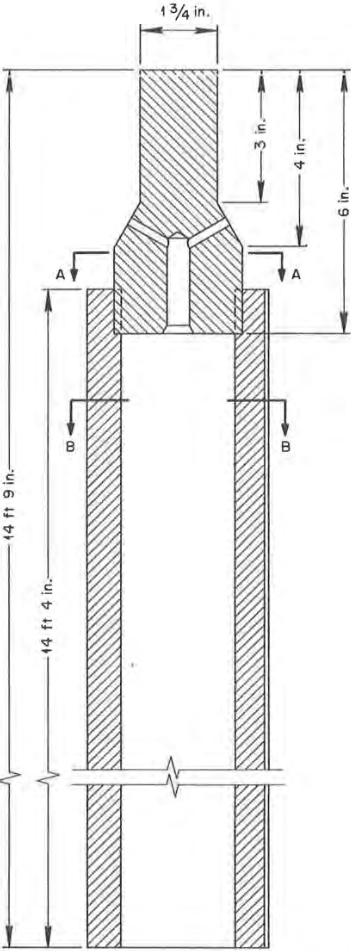
\includegraphics[width=0.25\linewidth]{figs/ch4/zone_iia_full_ref.png}
        \label{fig:msbr_iia_full_ref}
    }
    \subfloat[][]{
        
\includegraphics[width=0.17\linewidth]{figs/ch4/zone_iia_full_openmc.png}
        \label{fig:msbr_iia_full_model}
    }
    %\end{tabular}
    \caption[$xz$ cross sections of Zone II-A elements]{
        \subref{fig:msbr_iia_full_ref} Reference zone II-A element
        \subref{fig:msbr_iia_full_model} Model zone II-A element
    }
    \label{fig:msbr-iia-xz-full}
\end{figure}

\begin{figure}[htpb]
    \centering
    %\begin{tabular}{cc}
    \subfloat[][]{
        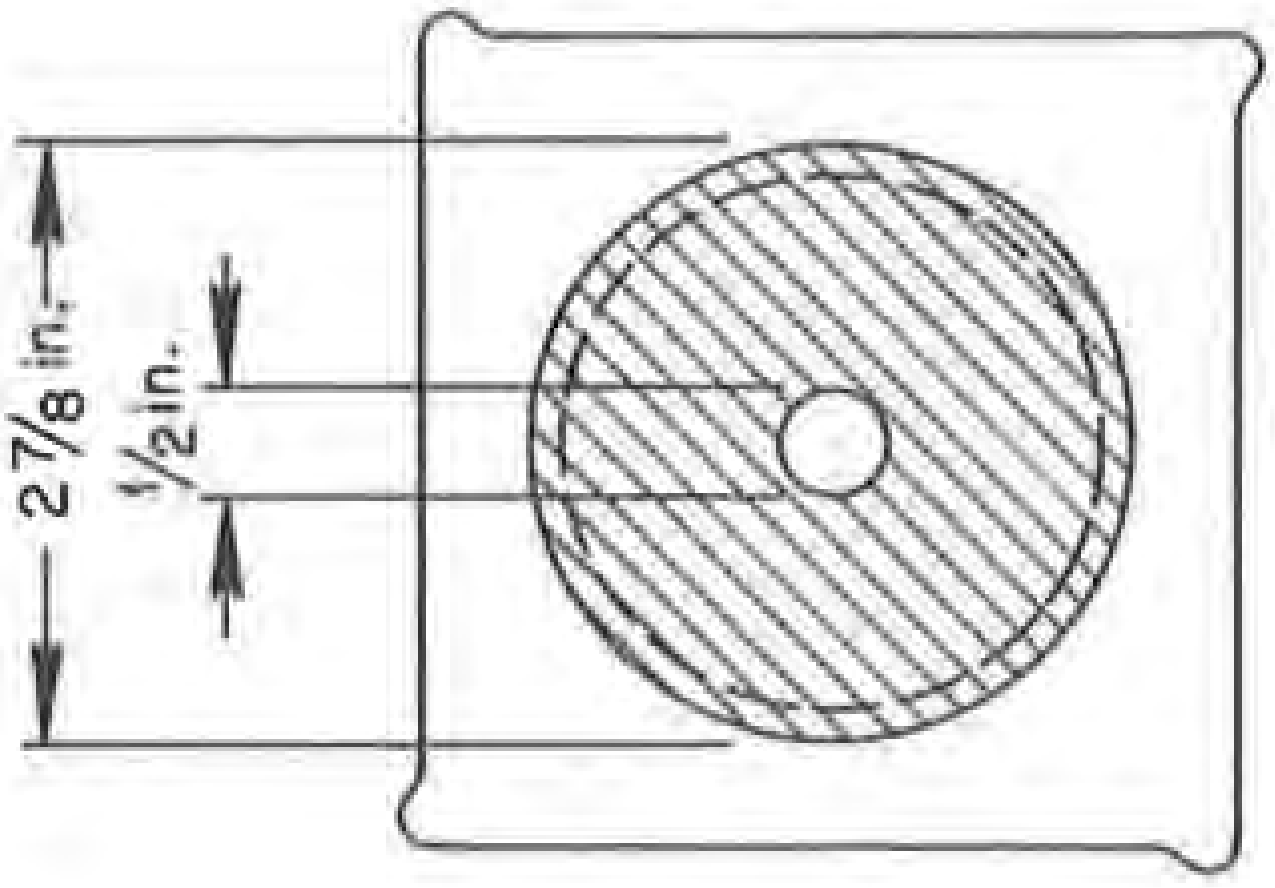
\includegraphics[width=0.3\linewidth]{figs/ch4/zone_iia_top_xy_ref.png}
        \label{fig:msbr_iia_top_ref}
    } 
    \subfloat[][]{
        
\includegraphics[width=0.2\linewidth]{figs/ch4/zone_iia_top_xy2_openmc.png}
        \label{fig:msbr_iia_top_model}
    }
    \\
    \subfloat[][]{
        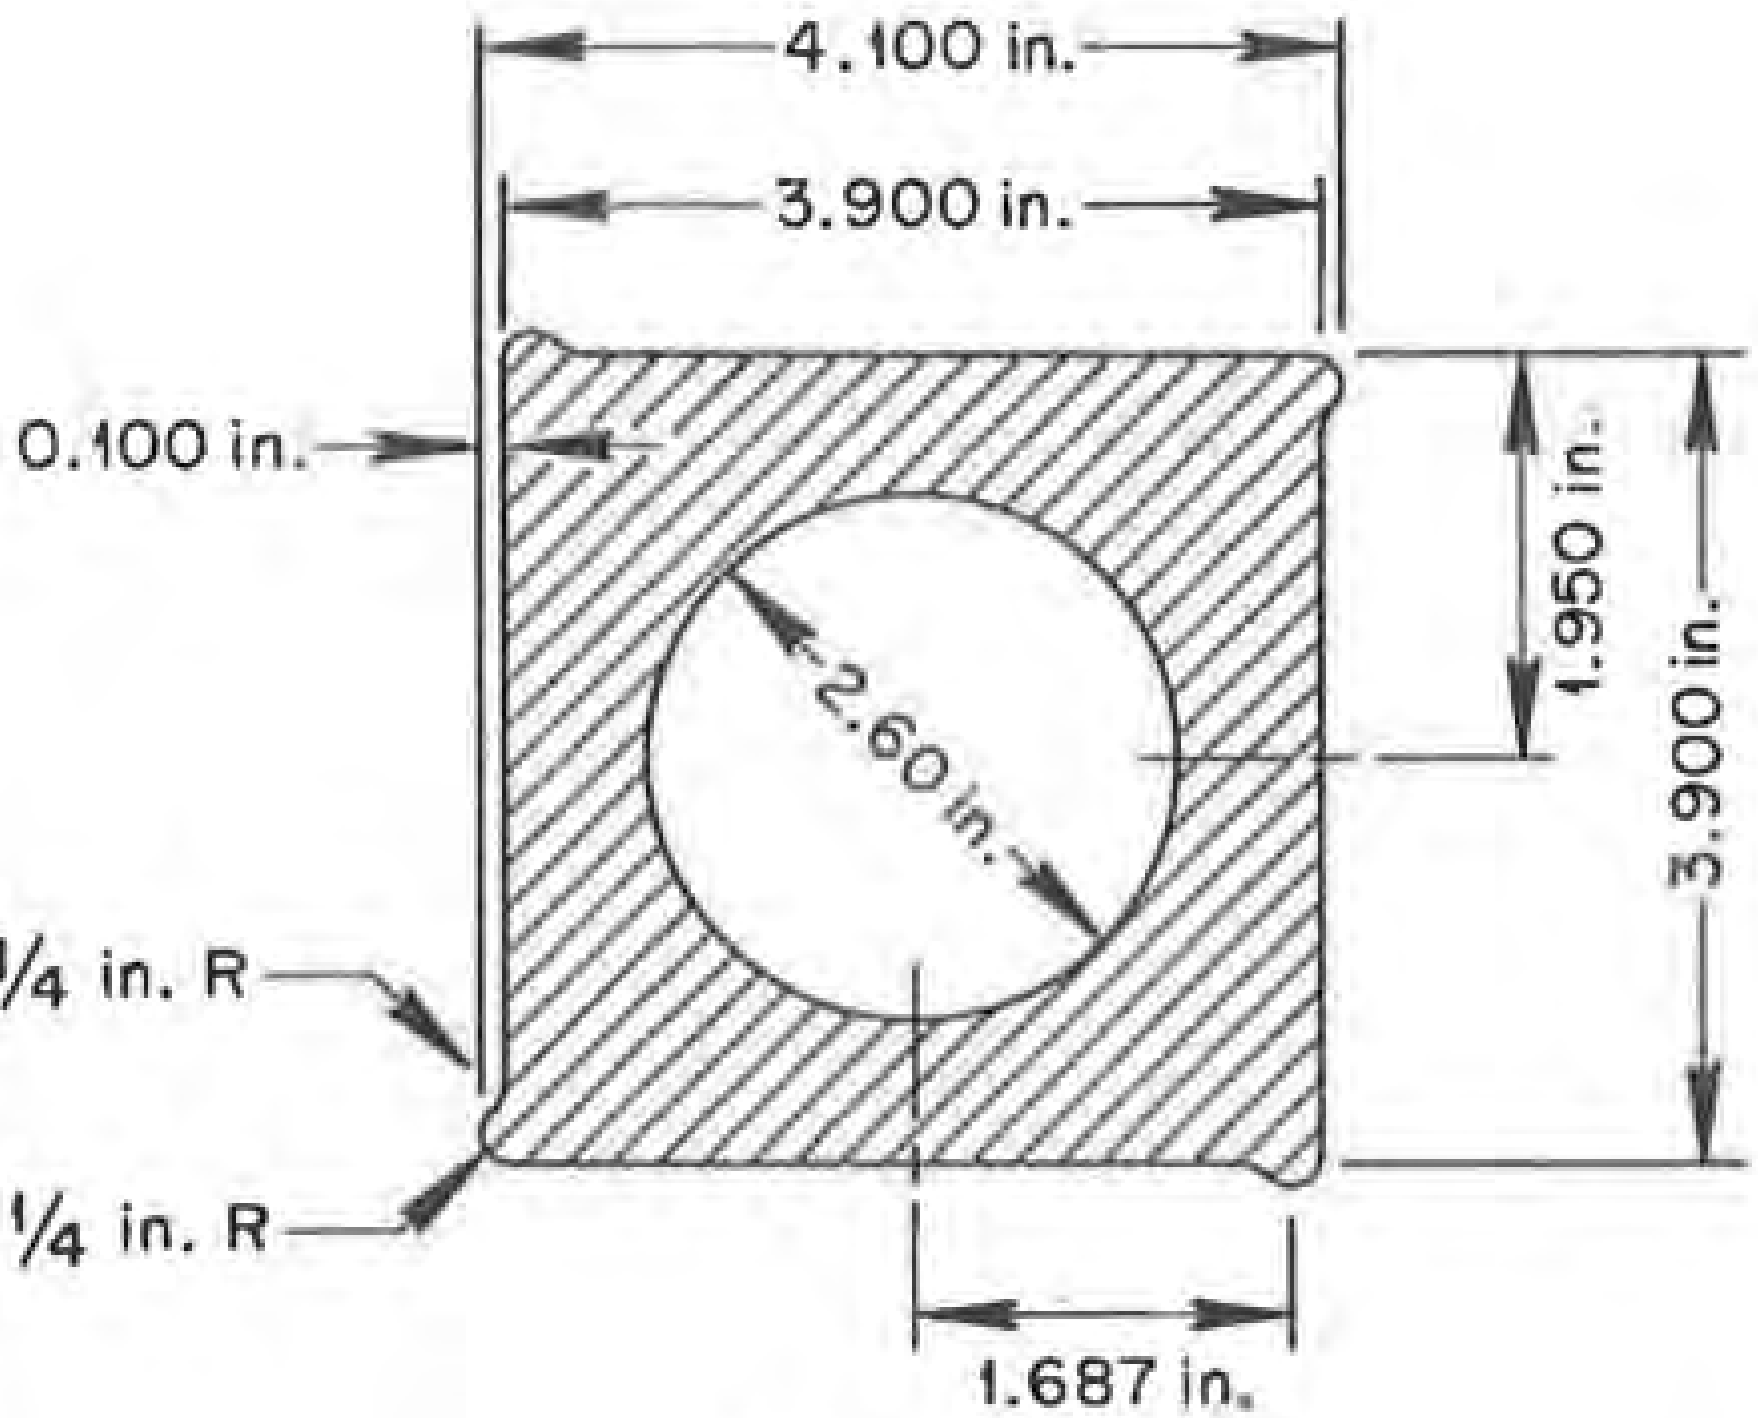
\includegraphics[width=0.35\linewidth]{figs/ch4/zone_iia_main_ref.png}
        \label{fig:msbr_iia_main_ref}
    } 
    \subfloat[][]{
        
\includegraphics[width=0.15\linewidth]{figs/ch4/zone_iia_main_openmc.png}
        \label{fig:msbr_iia_main_model}
    }
    %\end{tabular}
    \caption[$xy$ cross sections of Zone II-A elements]{
        \subref{fig:msbr_iia_top_ref} Reference zone II-A element; Section A.
        \subref{fig:msbr_iia_top_model} Model zone II-A element; Section A.
        \subref{fig:msbr_iia_main_ref} Reference zone II-A element; Section B.
        \subref{fig:msbr_iia_main_model} Model zone II-A element; Section B.
    }
    \label{fig:msbr-iia-xy}
\end{figure}

\subsection{Annulus}
A 2 in. wide annular space of 100-\% fuel salt separates zone II from the
graphite reflectors. The annulus serves as a clearance space when inserting or
removing the reactor core assembly, and provides some additional shielding to
extend the lifetime of the graphite reflectors \cite{robertson_conceptual_1971}. The annulus region is reproduced in full in the \Gls{csg} model. The annulus region is the dark teal section in between the brown and pink sections in Figure \ref{fig:msbr-cells}

\subsection{Reflectors}
\begin{figure}[htpb]
    \centering
    \subfloat[][]{
        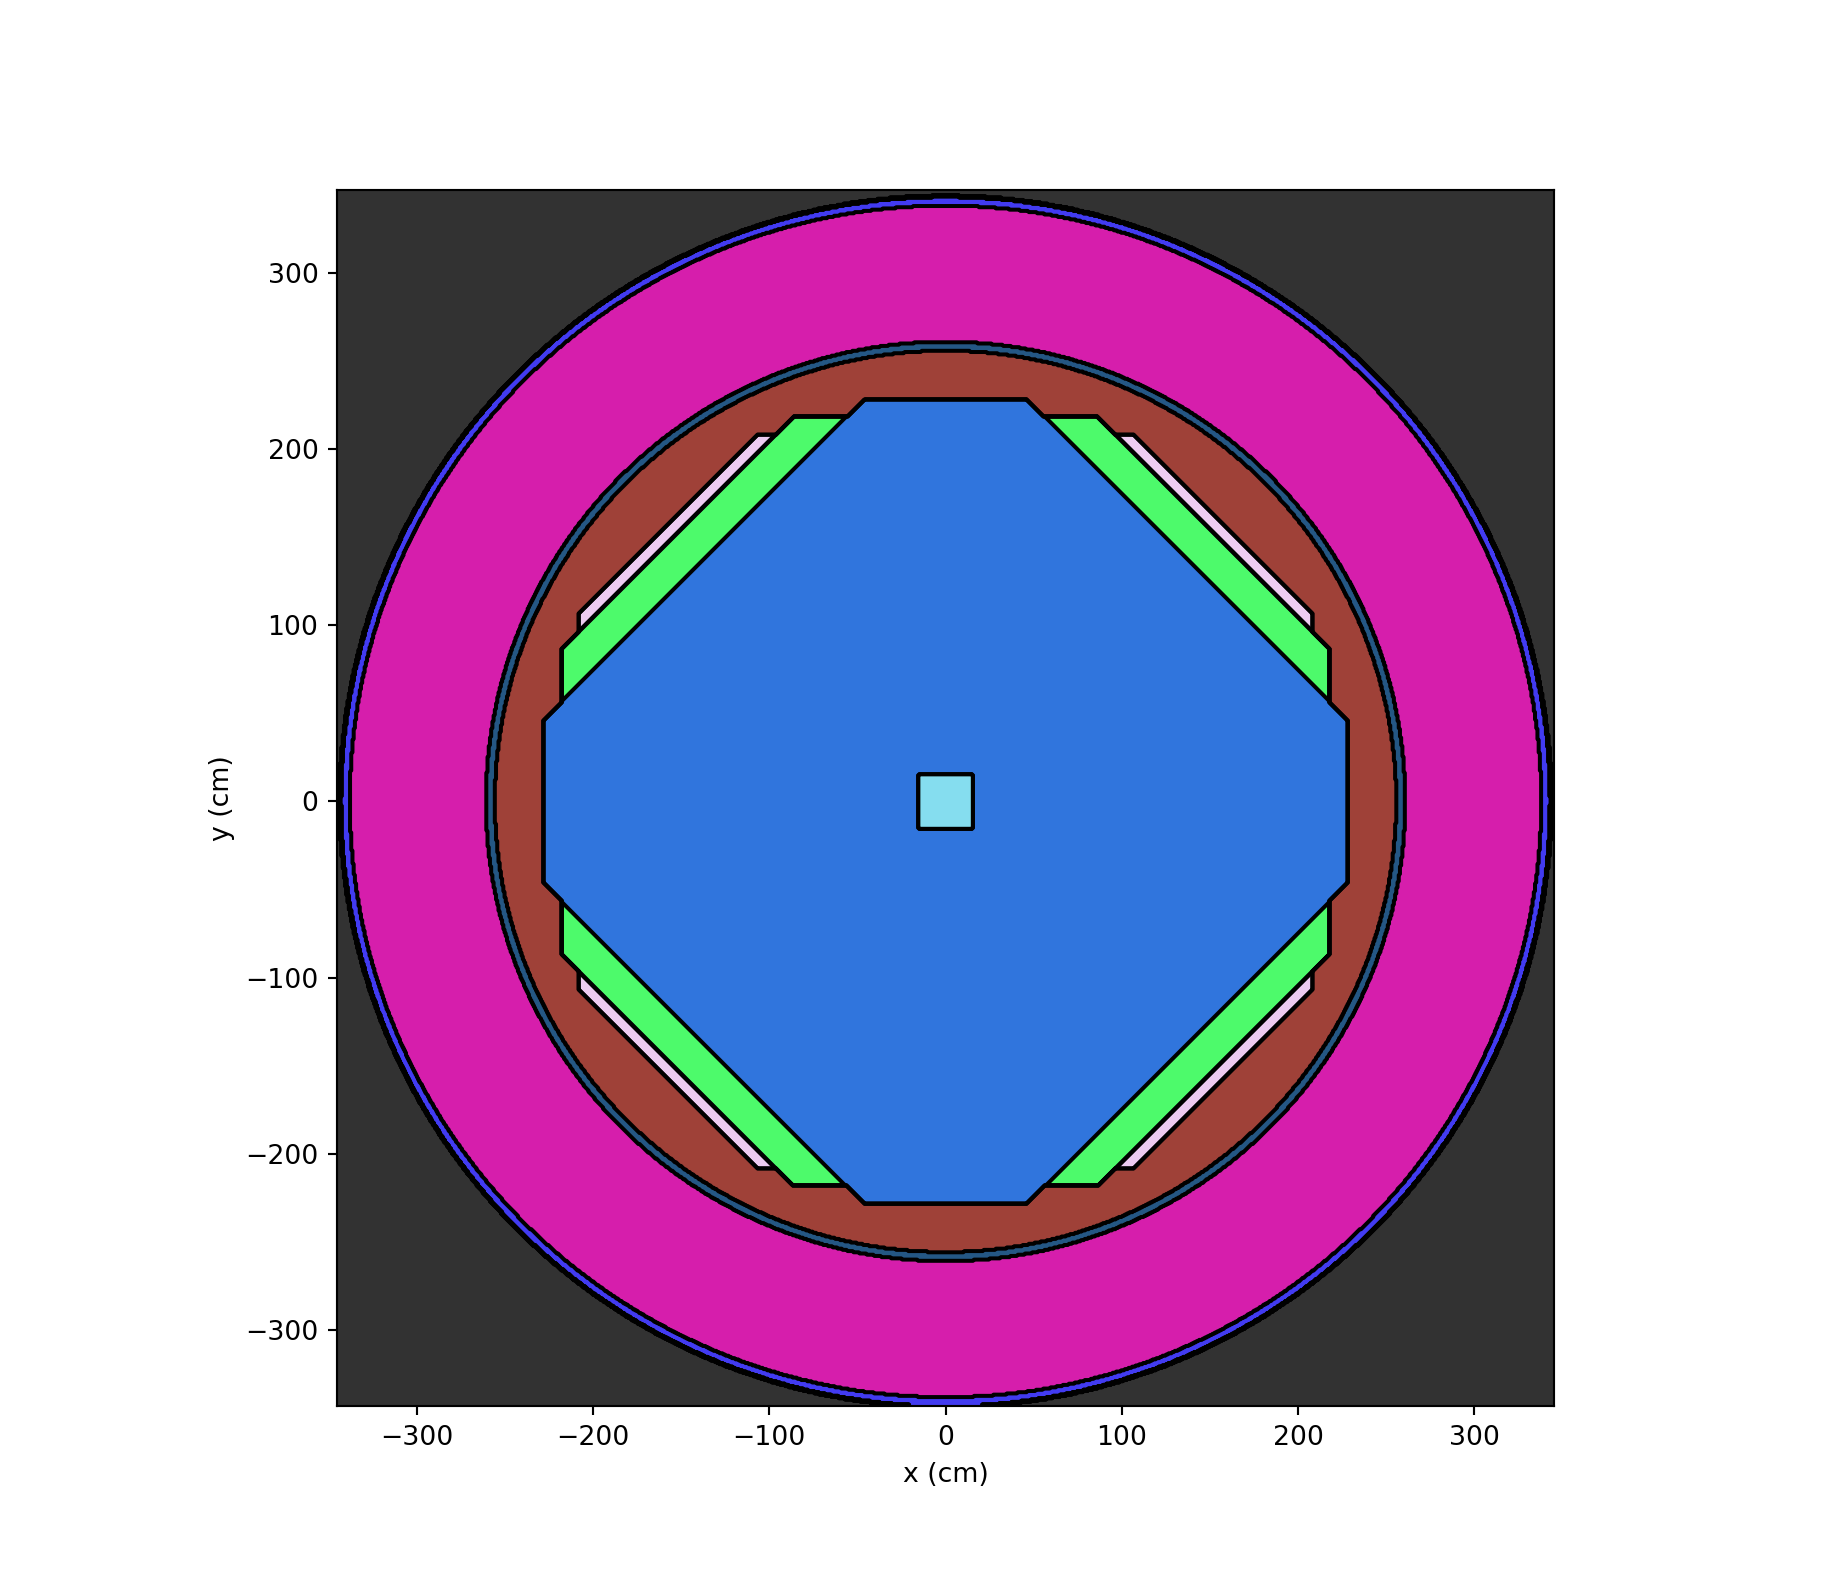
\includegraphics[width=0.5\linewidth]{figs/ch4/msbr_reduced_univs_xy.png}
        \label{fig:msbr-cell-xy}
    }
    \subfloat[][]{
        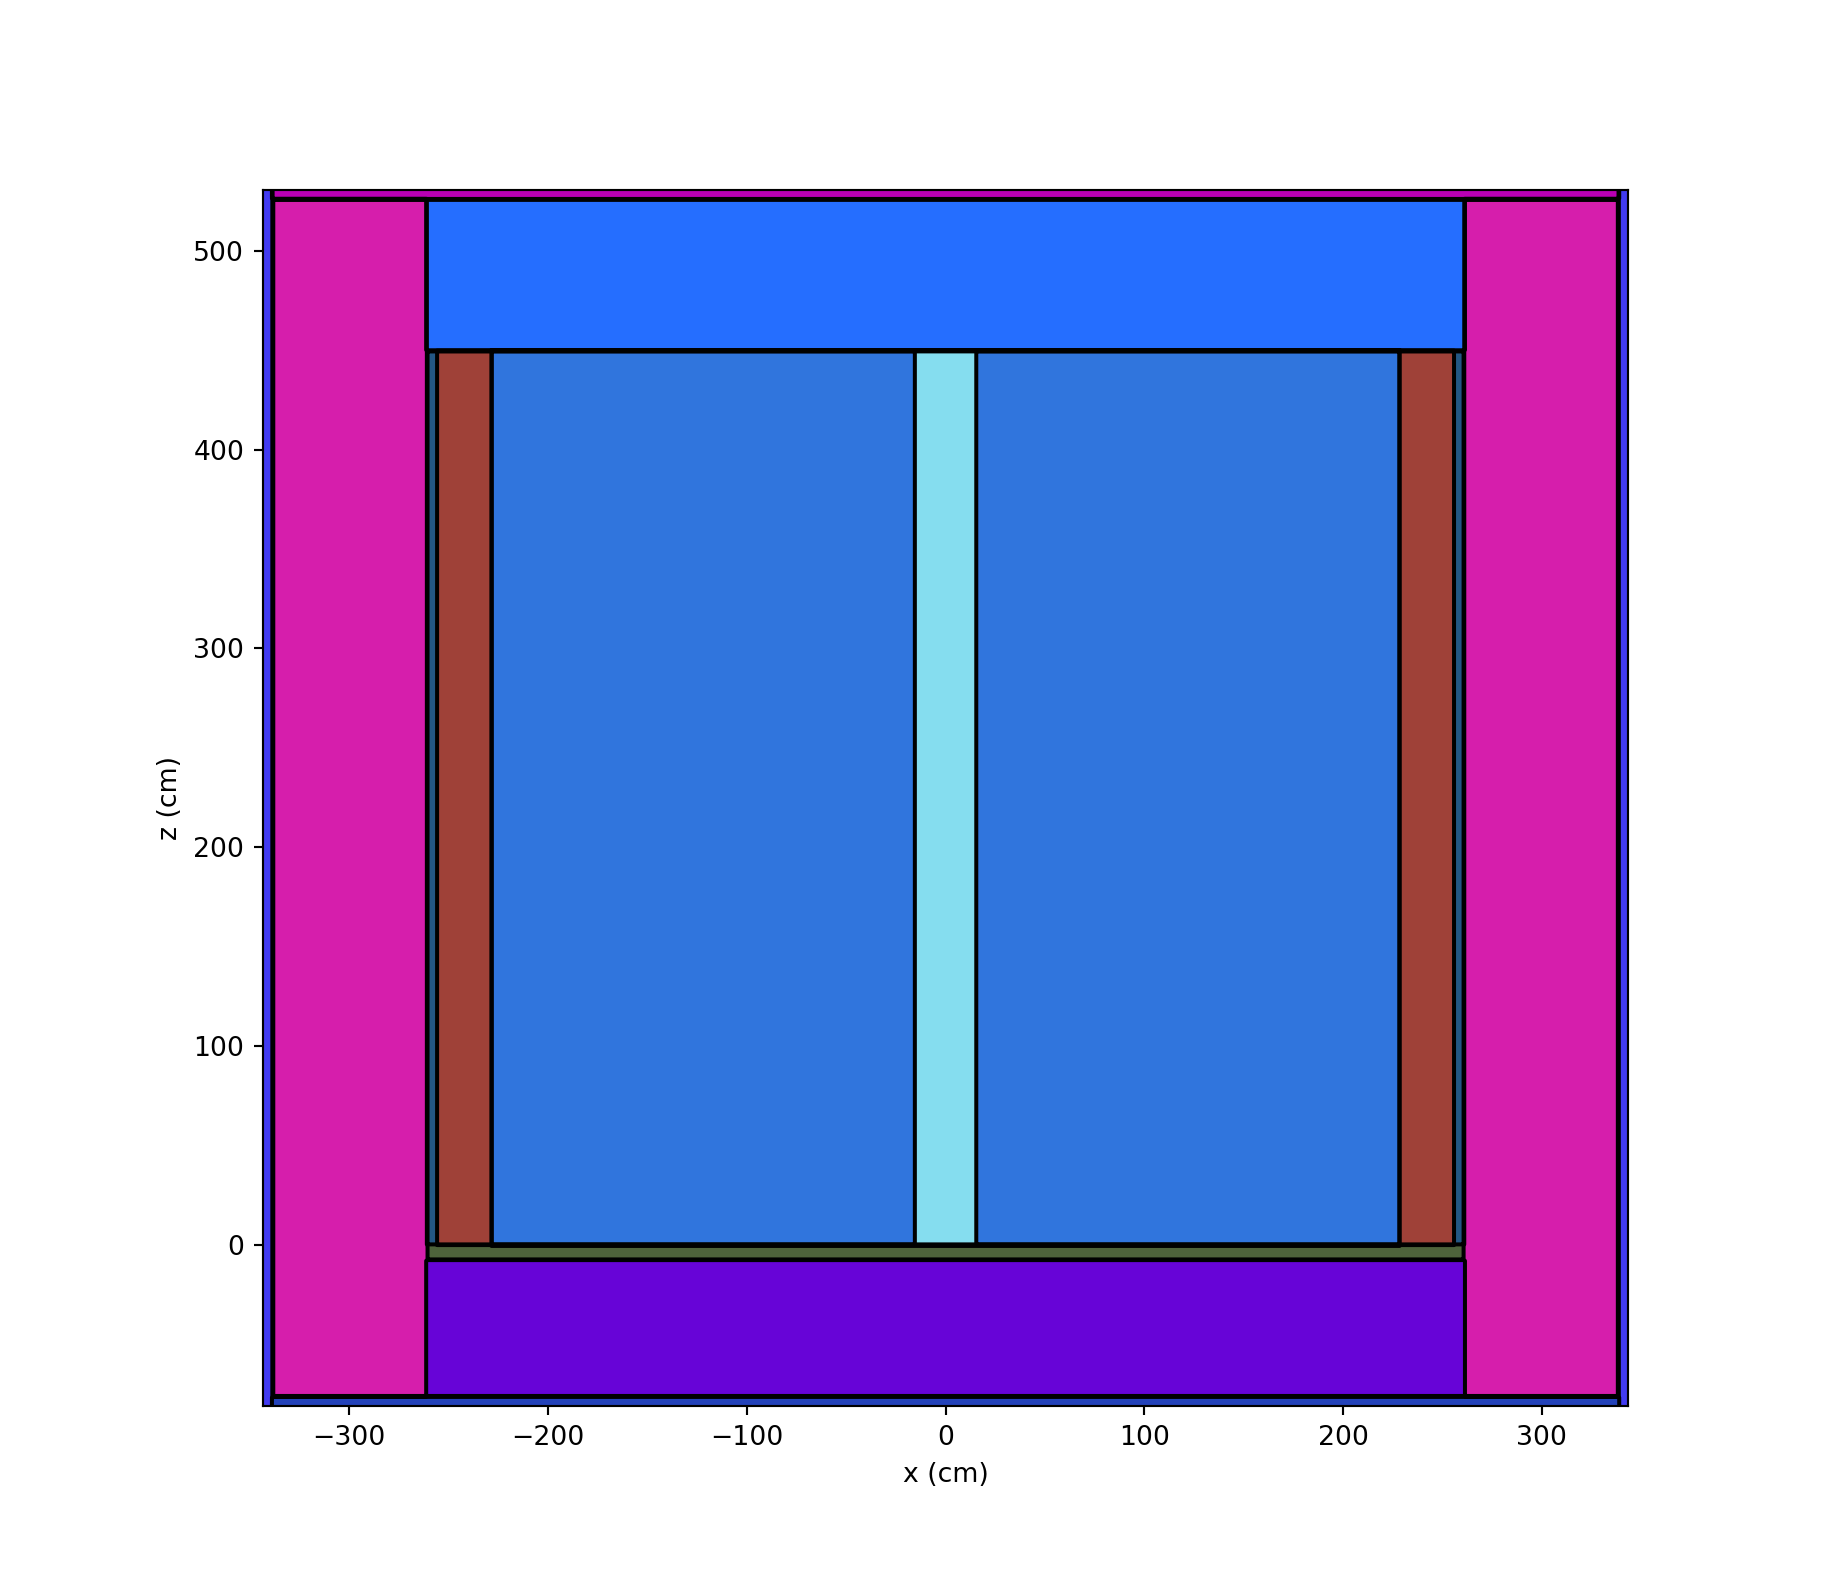
\includegraphics[width=0.5\linewidth]{figs/ch4/msbr_reduced_univs_xz.png}
        \label{fig:msbr-cell-xz}
    }
    \caption[MSBR CSG model cells]{MSBR CSG model cells.
        \subref{fig:msbr-cell-xy} $xy$ plane; 
        \subref{fig:msbr-cell-xz} $xz$ plane} 
    \label{fig:msbr-cells}
\end{figure}
The \Gls{msbr} has both axial and radial reflectors as seen in Figures
\ref{fig:msbr-overview} and \ref{fig:msbr-detail}. Both reflector regions are around 1\% fuel salt by volume. The radial
reflectors\footnote{I exclude the following details about the radial reflector
due to insufficient information in the report to reproduce them in a model:
modified Hastelloy N orifice plates, milled radial grooves at the bottom of each
reflector block, top layer blocks (see pages 15 and 16 in Robertson et al.
(1971))} consist of 29 in. (48.26 cm) thick wedge-shaped blocks that are 43 in. tall and 10 in. (25.4 cm) wide at the vessel wall and 9 in. wide at the inner end \cite{robertson_conceptual_1971}.
Four layers of these blocks comprise the entire radial reflector. Slots cut out
of the outer edge of the blocks facilitate modified Hastelloy N axial ribs to create a
0.25 in (0.635 cm) standoff space between the blocks and the vessel wall. Axial
flow from the reactor inlet through this space cools both the outer portion of
the reflector blocks and the vessel wall. Additionally, Robertson et al. (1971)
states that 1 in. graphite pins ``are inserted into the reflector pieces to hold
them apart'', but does not specify the position or number of these pins. These
pins create passages\footnote{these passages change dimension from 0.05 in. wide
while cold to 0.1 in. wide while hot \cite{robertson_conceptual_1971}} for
radial salt flow through the radial reflector region towards the annulus,
providing additional cooling. Modified Hastelloy N retaining rings placed in slots
between the block layers (see Figure \ref{fig:msbr-ref-xz}) ensure that the
position of the reflector blocks to the vessel wall stays relatively constant as
the materials expand under the heating of the fuel salt
\cite{robertson_conceptual_1971}.

The axial reflectors consist of wedge shaped graphite pieces (see Figure
\ref{fig:msbr-ref-xy}) that are 2 in. (5.08 cm) wide at the inner end and 16 in.
(40.64 cm) wide at the outer end \cite{robertson_conceptual_1971}. The dished
vessel heads cause the pieces to vary in thickness from 30 in. (76.2 cm) at the
center to 15 in. (38.1 cm) at the outer end (see Figure
\ref{fig:msbr-ref-xz}) \cite{robertson_conceptual_1971}. Robertson et al. (1971)
does not specify a length for the axial reflector pieces. 

The \Gls{csg} model approximates the complicated structure of the radial
reflector blocks as a hollow cylinder 601.98 cm tall and 77.216 cm thick, and
the axial reflector pieces as flat disks\footnote{the \Gls{csg} model does not
include the hole out of the top of the core for the control rods, and flattens
the dished shape as no dimensions are given to accurately reproduce the curvature
of the axial reflector pieces} 68.58 (bottom)/76.12 (top) cm thick and a radius
of 261.112 cm. The \Gls{csg} model also contains no fuel salt in the reflector
regions. Figure \ref{fig:msbr-cells} shows the radial reflector as a large pink
region, the top axial reflector as a light blue region, and the bottom axial
reflector as a purple region.

\section{Vessel}
\label{sec:msbr-vessel}
The \Gls{msbr} vessel is made of modified Hastelloy N, and has a wall thickness
of 2 in. unless otherwise specified \cite{robertson_conceptual_1971}. The vessel
is broken into the following sections:
\begin{enumerate}
    \item The main wall: a 13 ft. tall cylindrical section with an outer
    diameter of 22.5 ft. This section is the main contact surface for the axial
    reflectors.
    \item The transition section: A 4 ft. tall conical section. The conical base
    has a diameter of ~22.5 ft. and the conical ``roof'' has a diameter of ~18
    ft. This section connects the main wall to the support section and contains
    the salt outlet nozzles.
    \item The nested support sections: two ~13.5 ft tall cylindrical sections
    that nest. Both sections have a 2 in. wall thickness. The outer cylinder has
    an inner diameter of 18 ft, and the inner cylinder has an outer diameter of
    slightly less than 18ft to allow for clearance to fit the two pieces
    together. The assembly is flanged at the top to close the vessel. The
    flanged support section is also the main point of contact with the
    reinforced concrete roof structure from which the reactor hangs.
    \item The dished head sections: both heads have a 3 in. wall thickness. The
    lower head has a 22.5 ft diameter and the upper head an 18 ft. diameter. No
    radius of curvature is given for the dished heads, but it may be possible to
    determine the shape using the given dimensions and other dimensions of the
    vessel.
\end{enumerate}

The CSG model representation of the vessel has a 2 in. (5.08
\unit{\centi\metre}) thickness, and hugs the radial region in the CSG model,
giving an outer diameter of 22.53 ft. (686.816 \unit{\centi\metre}) and a
height of 20.08 ft (612.14 \unit{\centi\metre}). The CSG model does not include
the nested support sections as they are of little neutronic importance. Figure
\ref{fig:msbr-cells} shows the radial vessel as a thin blue region at the outer
edge of the radial reflector region, and the axial vessel as a thin pink region
at the outer edge of the axial reflector regions.

\section{An aside on the salt volume}
\label{sec:salt-volume}
The original salt volume in the \Gls{csg} \Gls{msbr} model was set to
$4.871\cdot 10^7$ \unit{\centi\metre\cubed}. This is roughly double the salt
volume in the core in the reference specification (see Table
\ref{tab:salt-volumes}). I performed stochastic volume calculations on both the
\SerpentTWO and \OpenMC versions of the \Gls{csg} model, and found they both
calculated volumes around $2.6\cdot 10^7$ \unit{\centi\metre\cubed}. Averaging
the two volumes gives a roughly 8\% error in the salt volume in the core compared
to the reference specification (see Table \ref{tab:stoch-vol}).

\begin{table}[htpb]
    \centering
    \caption[MSBR fuel stochastic volume calculations]{MSBR fuel stochastic volume calculations, using $1\cdot 10^9$ particles.}
    \label{tab:stoch-vol}
    \begin{tabular}{|c|c|c|c|}
        \hline
        Quantity & \SerpentTWO & \OpenMC & Average\\
        \hline
        Volume [\unit{\centi\metre\cubed}] & $2.60961 \cdot 10^7$ & $2.6085 \cdot 10^7$ & $2.6091 \cdot 10^7$ \\
        \hline
        Statistical error & 0.00010 & 0.00010 & 0.00007 \\
        \hline
    \end{tabular}
\end{table}

For depletion without reprocessing this new volume would be correct to
use for our geometry. When we assume that we are performing online reprocessing,
we must account for all of the salt in the core {\it and} the salt in the
primary loop as this salt is routed through the processing components. Table S.1
in \cite{robertson_conceptual_1971} gives us the total volume of salt in the
primary system as  1720 ft$^{3}$ ($4.8705\cdot 10^7$ \unit{\centi\metre\cubed}).
This value is valid assuming that we have reproduced the core geometry exactly
as specified, however in the \Gls{msbr} reference design, the total volume of
salt in the reactor vessel is 1074 ft$^{3}$ ($3.0412 \cdot 10^{7}$
\unit{\centi\metre\cubed}) \cite{robertson_conceptual_1971}, which is 
approximately 13\% greater than the geometrical volume of the salt. This
discrepancy is due to the absence of the core inlets, outlets, and the narrow
salt passages in the reflector region. These features are important for thermal
hydraulic accuracy, however they are most likely not particularly neutronically
important. Additionally, we want to stay as consistent as possible with
Rykhlevskii's previous works \cite{rykhlevskii_fuel_2020}
\cite{rykhlevskii_modeling_2019}, so we will use the existing value for the salt
volume of $4.871\cdot 10^7$. \unit{\centi\metre\cubed}. This choice carries the
implicit assumption that we are applying the neutronic conditions in the core to
$4.871\cdot 10^{7}$ \unit{\centi\metre\cubed} of salt during the entire
depletion step, which does not account for the actual salt processing rate and
fuel salt mass flowrate\footnote{According to Table S.1 in Robertson et al.
(1971), the cycle time for the salt inventory in the primary system is 10 days
\cite{robertson_conceptual_1971}}. To do so would require development of
SaltProc that is outside the scope of this thesis.

%% Table 3.2 and 3.3 in robertson
\begin{table}[htpb]
    \centering
    \caption[Volume of salt in reference MSBR core regions]{Volume of salt in
reference MSBR core regions. Reproduced from Table 3.2 in
\cite{robertson_conceptual_1971}}
    \label{tab:salt-volumes}
    \begin{tabular}{|c|c|cc|}
        \hline
        Zone & Percent salt & Salt volume [ft$^3$] & Salt volume [\unit{\metre\cubed}] \\
        \hline
        Zone I & 13.2 & 288 & 8.155252 \\
        \hline
        Zone II & 37 & 376.5 & 10.661293 \\
        \hline
        Upper plenum & 85 & 36.2 & 1.02507 \\ 
        \hline
        Lower plenum & 100 & 35.4 & 1.002416 \\ 
        \hline
        Annulus & 100 &  132 & 3.737824\\
        \hline
        Core total & - & 868.1 & 24.581855 \\ 
        \hline
    \end{tabular}
\end{table}

\section{Reprocessing system}
\label{sec:msbr-reprocessing-system}
The MSBR reference design included the specification of a fuel-salt processing
system\footnote{For this thesis, processing refers to both gas removal and
chemical processing}. The purpose of this reprocessing system is to improve
neutronic performance by removing neutron poisons and other contaminants from
recirculating through the core. The reprocessing system is split into two parts:
gas removal and chemical extraction. The gas removal system takes advantage
of entrainment of insoluble species in helium bubbles to remove noble gas
fission products from the fuel salt. The reprocessing system is based on
reductive extraction\footnote{Reductive extraction takes advantage of the higher
electronegativity of a particular element to drive reduction reactions that
remove target elements from covalently bonded molecules}. I will provide a brief
description of the entire reprocessing system, but justifying in and evaluating
its efficacy are beyond the scope of this thesis\footnote{I encourage interested
readers to look at chapters 7 and 8 in \cite{robertson_conceptual_1971}, the
entirety of \cite{carter_design_1972} and \cite{lindauer_design_1969}, as well
as the molten salt reactor program semiannual progress reports, all of which you
can find at \url{energyfromthorium.com/pdf}}.

\begin{figure}[htpb]
    \centering
    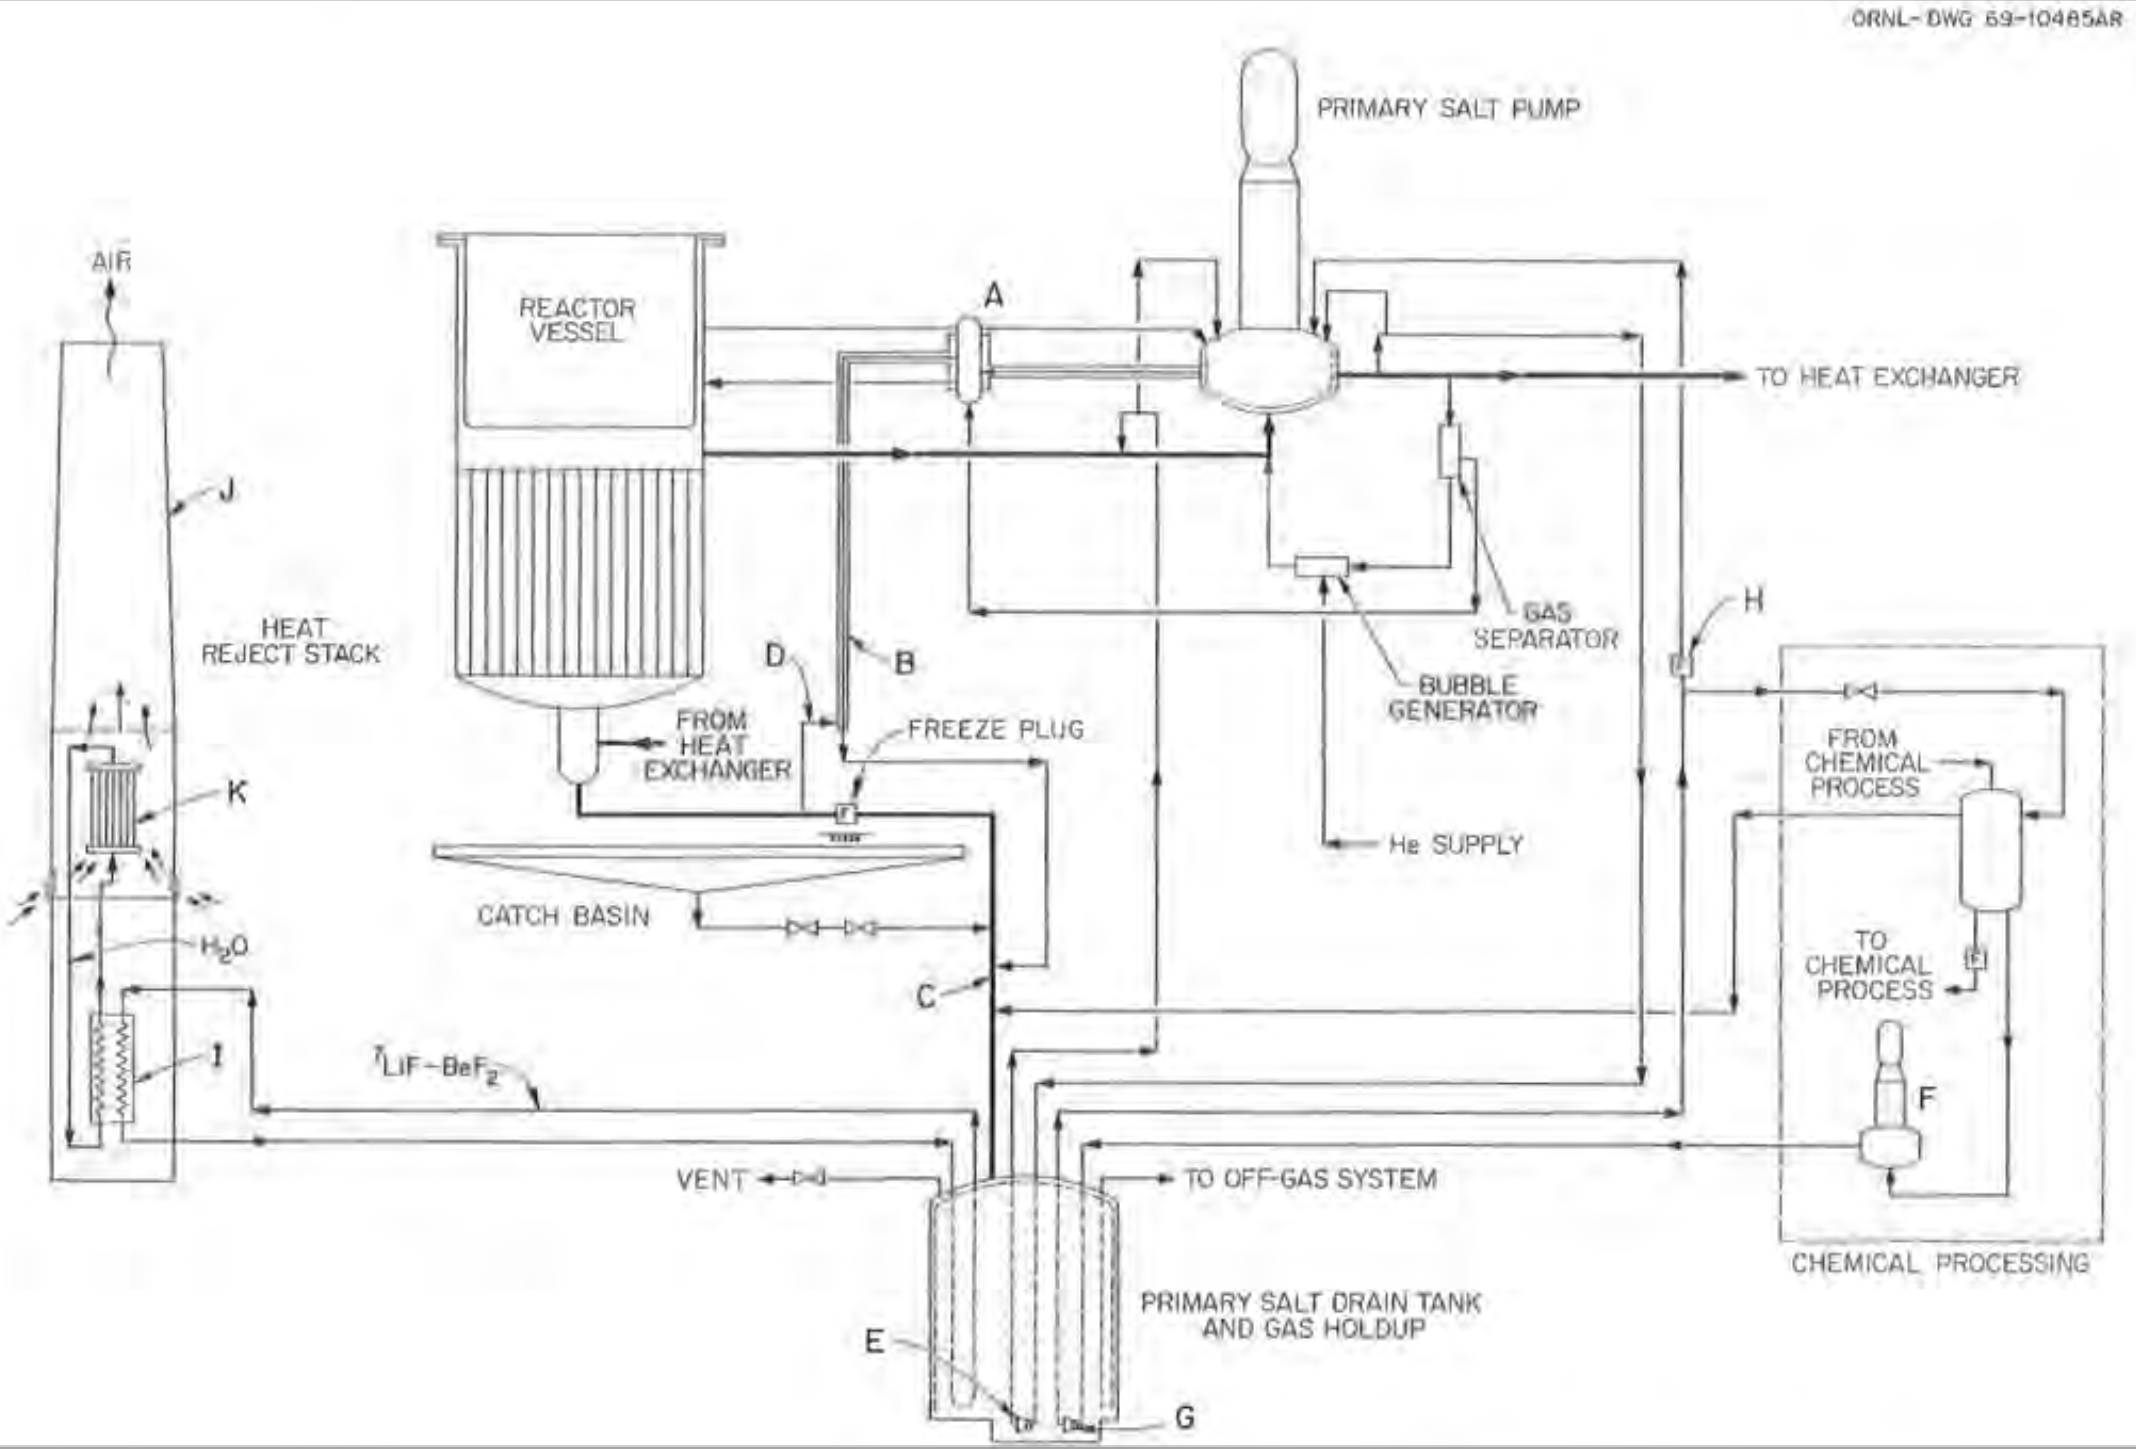
\includegraphics[width=0.8\textwidth]{figs/ch4/msbr_primary_system.png}
    \caption[Simplified flow diagram of primary drain tank and heat removal
    system.]{Simplified flow diagram of primary drain tank and heat removal
    system. Reproduced from Figure 2.3 in \cite{robertson_conceptual_1971}. (A)
    Combiner tank for separated gases and overflow salt, (B) Off-gas line with
    cooling jacket, (C) Fuel-salt drain line, (D) Drain line continuous bleed
    flow, (E) Jet pumps from returning overflow fuel salt to primary system, (F)
    Ancillary fuel-salt transfer pump, (G) Jet pump for filling primary system
    and sending salt to chemical processing, (H) Freeze-plug type valve }
    \label{fig:msbr_primary_system}
\end{figure}

\subsection{Gas removal system}
The gas removal system removes short-lived neutron poisons gases (tritium,
xenon, and krypton) from returning to the core region. There are three
components to this system: the bubble generator, the gas separator, and the
off-gas system. The gas separator is where the physical separation of the
neutron poisons from the fuel salt occurs.

The bubble generator creates bubbles from helium gas injected into the fuel
salt\footnote{the phenomena of pockets of gas trapped in pockets, along with any
other material they may pick up, and transported in fluid flow is called {\it
entrainment}. The \Gls{msbr} includes a salt entrainment separator downstream
from the gas separator that removes entrained salt and metal contaminants from
the helium bubbles before the gas is processed. See Section 5.3 in
\cite{rosenthal_molten-salt_1968}}. These helium bubbles will pick up the
fission product gases and carry them on the interface between the helium and the
salt. This process is called {\it sparging}. Around 10\% of the total salt flow
is routed from the primary pumps into this system. Figure
\ref{fig:gas_removal_system} provides an overview.

\begin{figure}[htpb]
    \centering
    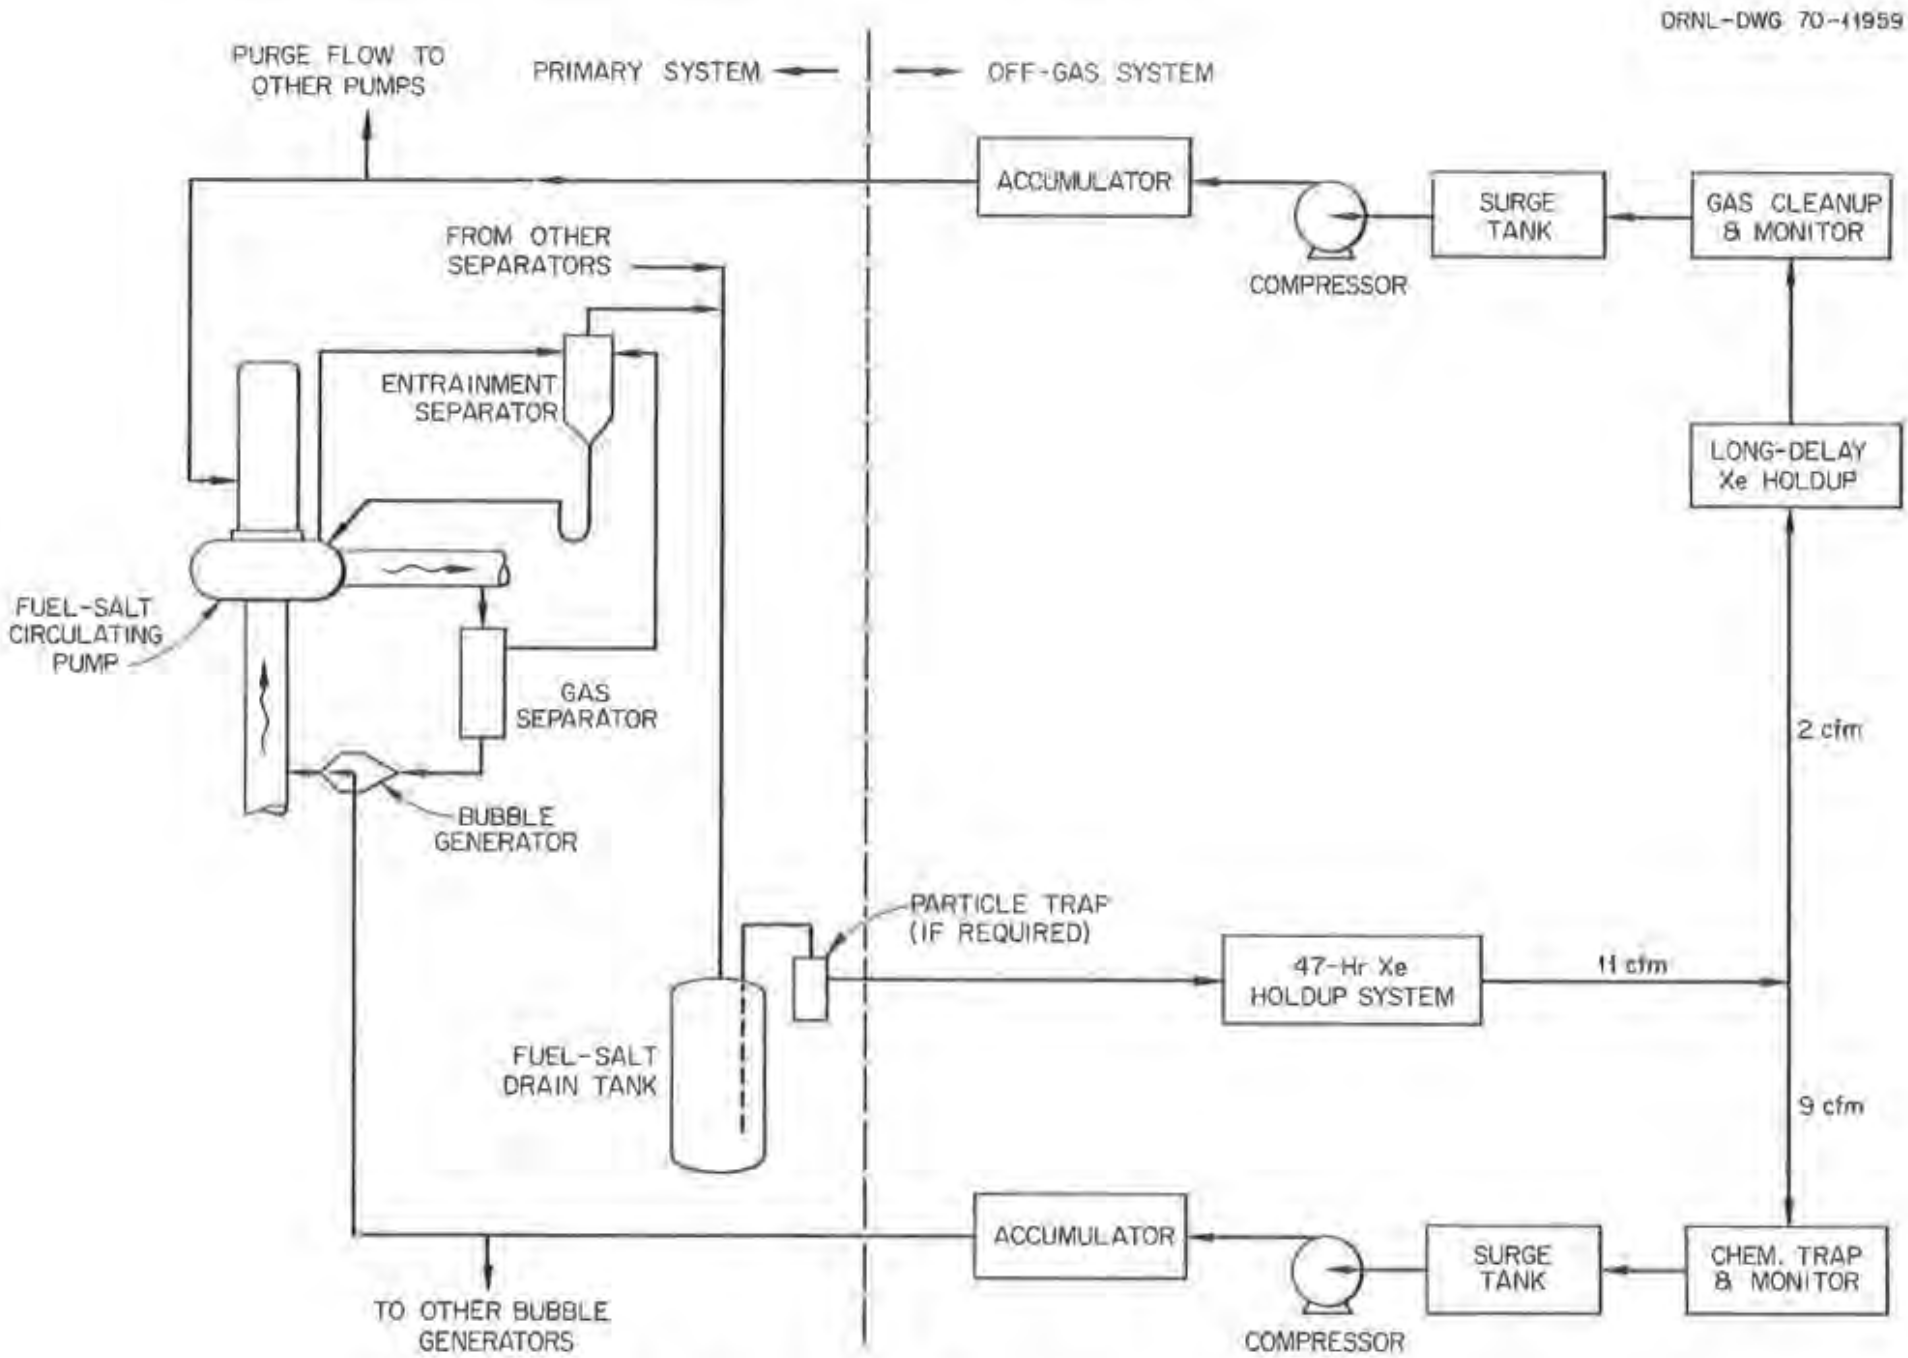
\includegraphics[width=0.8\textwidth]{figs/ch4/gas_removal_system.png}
    \caption{Overview of \Gls{msbr} gas removal system. Reproduced from Figure 7.1 in \cite{robertson_conceptual_1971}}
    \label{fig:gas_removal_system}
\end{figure}

The main purpose of the off-gas system is to separate the helium from the
fission product gasses for reuse in sparging. We only care about the
corresponding extraction efficiency of the fission product gases, so we do
not include the off-gas system in our model. Interested readers should reference
Chapter 7 in Robertson et al. (1971) \cite{robertson_conceptual_1971}.

\subsection{Fuel salt drain tank}
The fuel salt drain tank provides an emergency salt storage system in the case of
electrical system failure. Additionally, the fuel salt drain tank plays an important role in
the fuel-salt reprocessing system \cite{robertson_conceptual_1971}. The drain tank catches around 150 gpm (approximately 0.9\% of the total salt flow) of
overflow from the primary salt circulation pumps, providing it with a small
amount of salt during operation \cite{robertson_conceptual_1971}. A 0.88 gpm
stream of salt from the drain tank flows through the chemical processing system
and back to the drain tank. Jet pumps at the bottom of the drain tank send salt
back to the primary loop. Figure \ref{fig:msbr_primary_system} shows this
arrangement.

\subsection{Chemical processing system}
The chemical processing system has two purposes:
\begin{enumerate}
    \item To isolate \ce{^{233}Pa} from the high neutron flux zone to allow it to decay into \ce{^{233}U}
    \item To remove impurities (rare earth metals) and fission products from the fuel salt
\end{enumerate}

\begin{figure}[htpb]
    \centering
    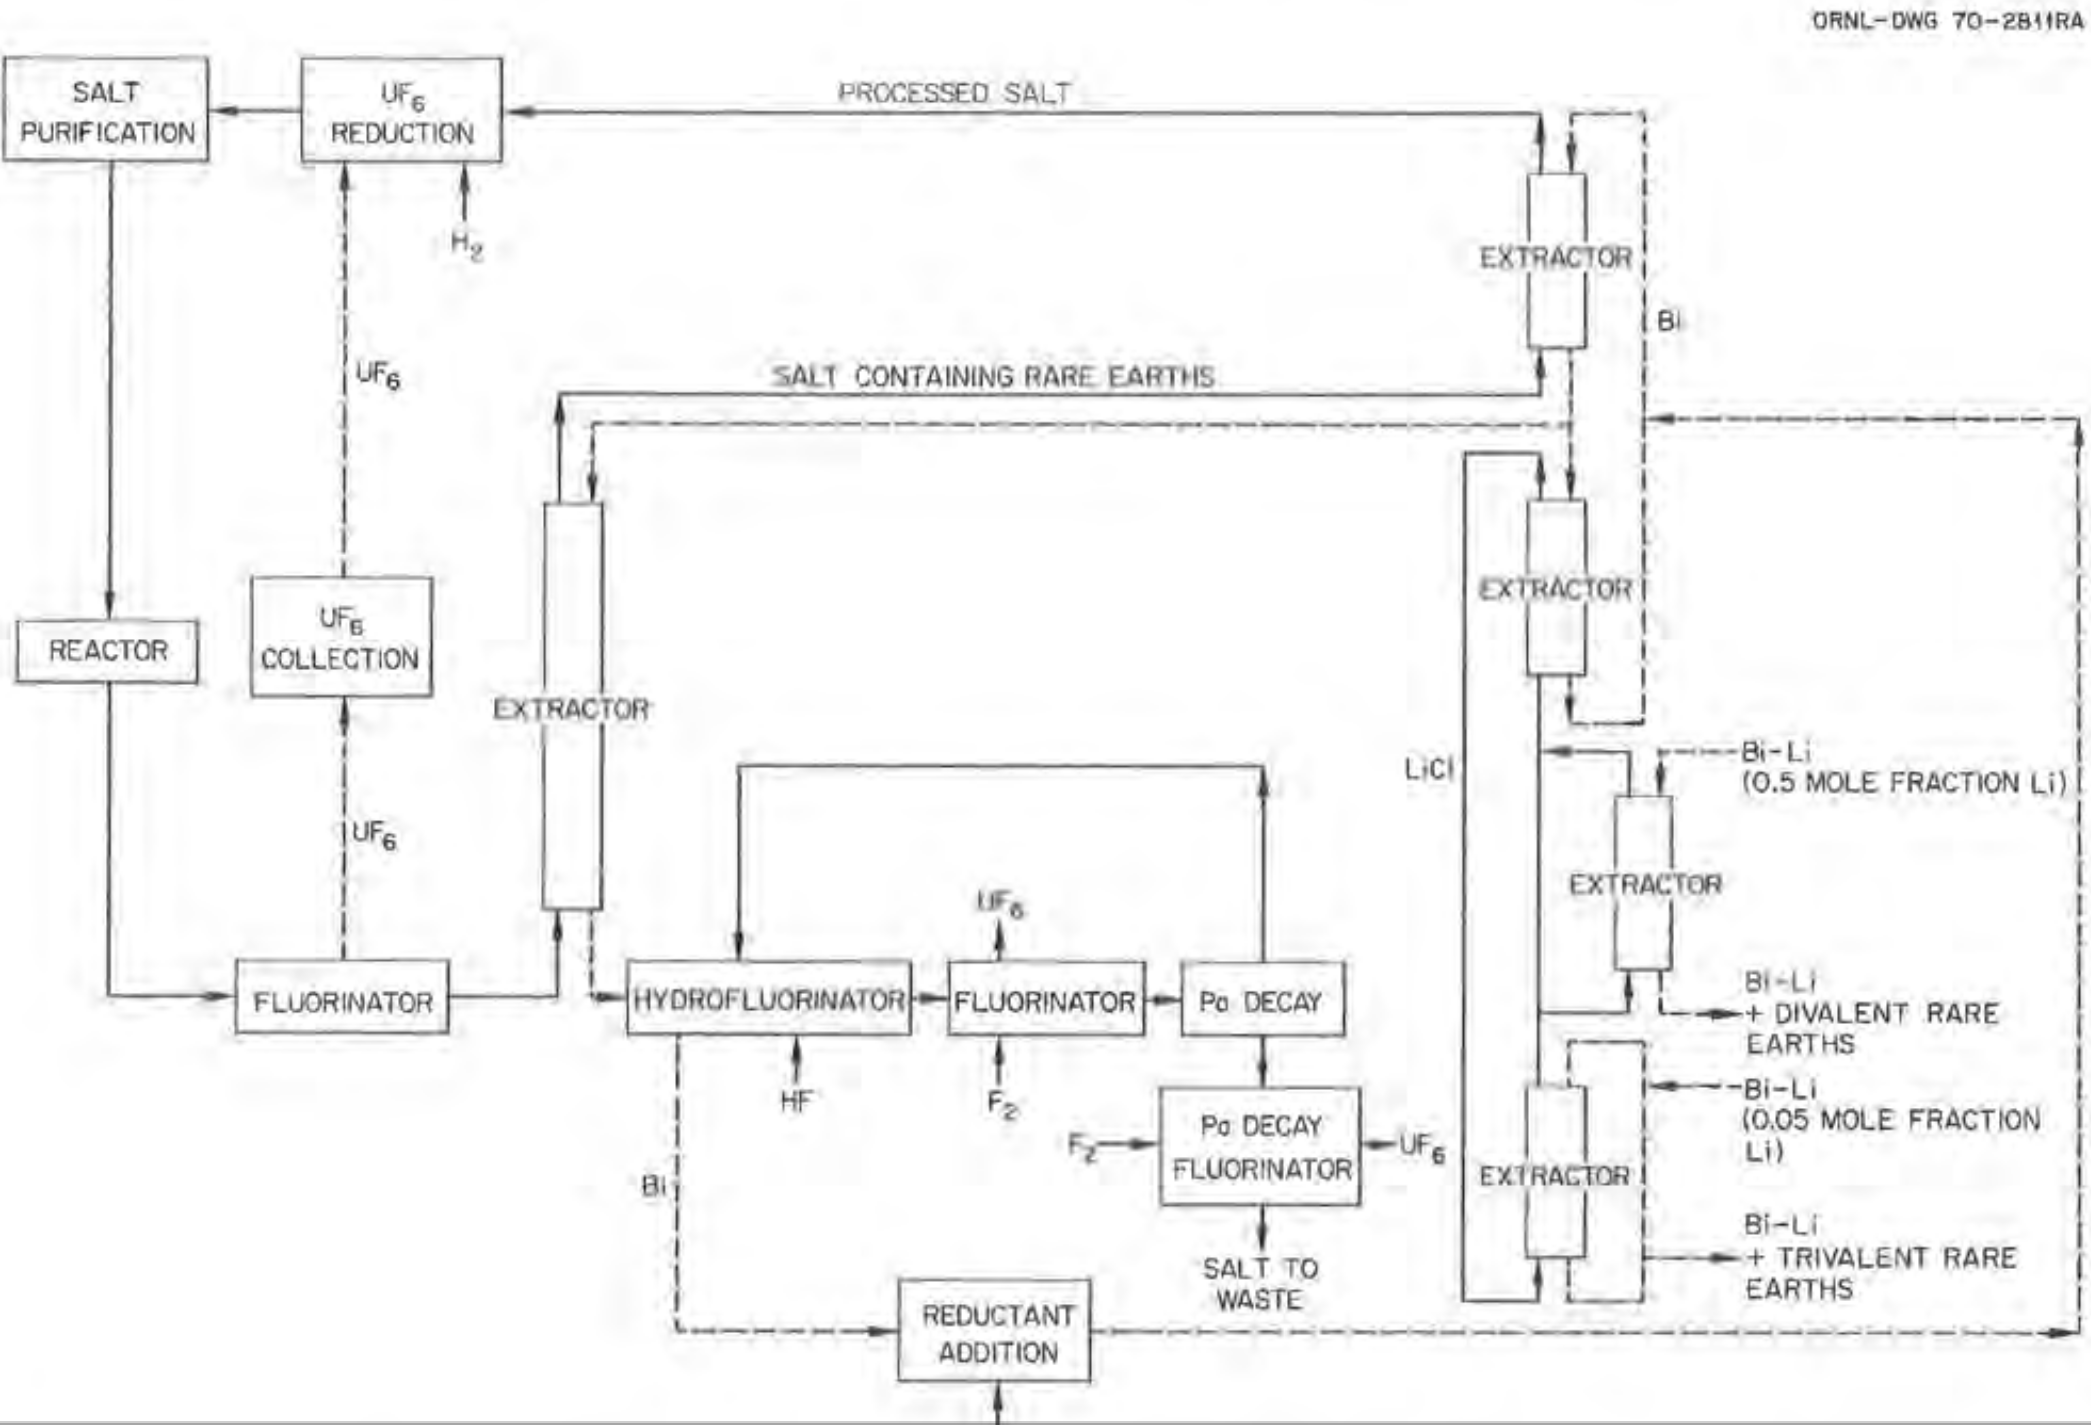
\includegraphics[width=0.8\textwidth]{figs/ch4/chemical_processing_system.png}
    \caption{Chemical processing system overview. Reproduced from Figure 2.4 in \cite{robertson_conceptual_1971}}
    \label{fig:}
\end{figure}

\paragraph{Protactinium isolation loop}
In order to remove the protactinium from the fuel salt, all uranium must first be removed. The protactinium isolation loop consists of several components: 
\begin{enumerate}
    \item A fluorinator to remove 95\% of the uranium in the fuel salt.
    \item An extraction column where the stream leaving the fluorinator is combined with a stream of bismuth and thorium that removes protactinium and additional uranium from the fuel salt. The salt stream leaving the extractor is routed to the rare metal removal system. This salt stream has nearly no protactinium or uranium in it.
    \item A hydrofluorinator where the stream leaving the extraction column removes the thorium, lithium, and uranium from the bismuth. The bismuth is sent to a reductant adder where lithium is added to the bismuth stream, and then is rerouted back to the extraction column.
    \item A second fluorinator that removes 95\% of the remaining uranium from the stream leaving the extraction column.
    \item A protactinium decay tank into which the stream leaving the second fluorinator flows. This stream is circulating as it feeds back to the hydrofluorinator for additional uranium removal. Uranium produced by protactinium decay is removed by this circulating stream.
\end{enumerate}

The uranium extracted via fluorination is returned to 
Figure \ref{fig:pa-removal} shows a block diagram of this loop. 

\begin{figure}[htpb]
    \centering
    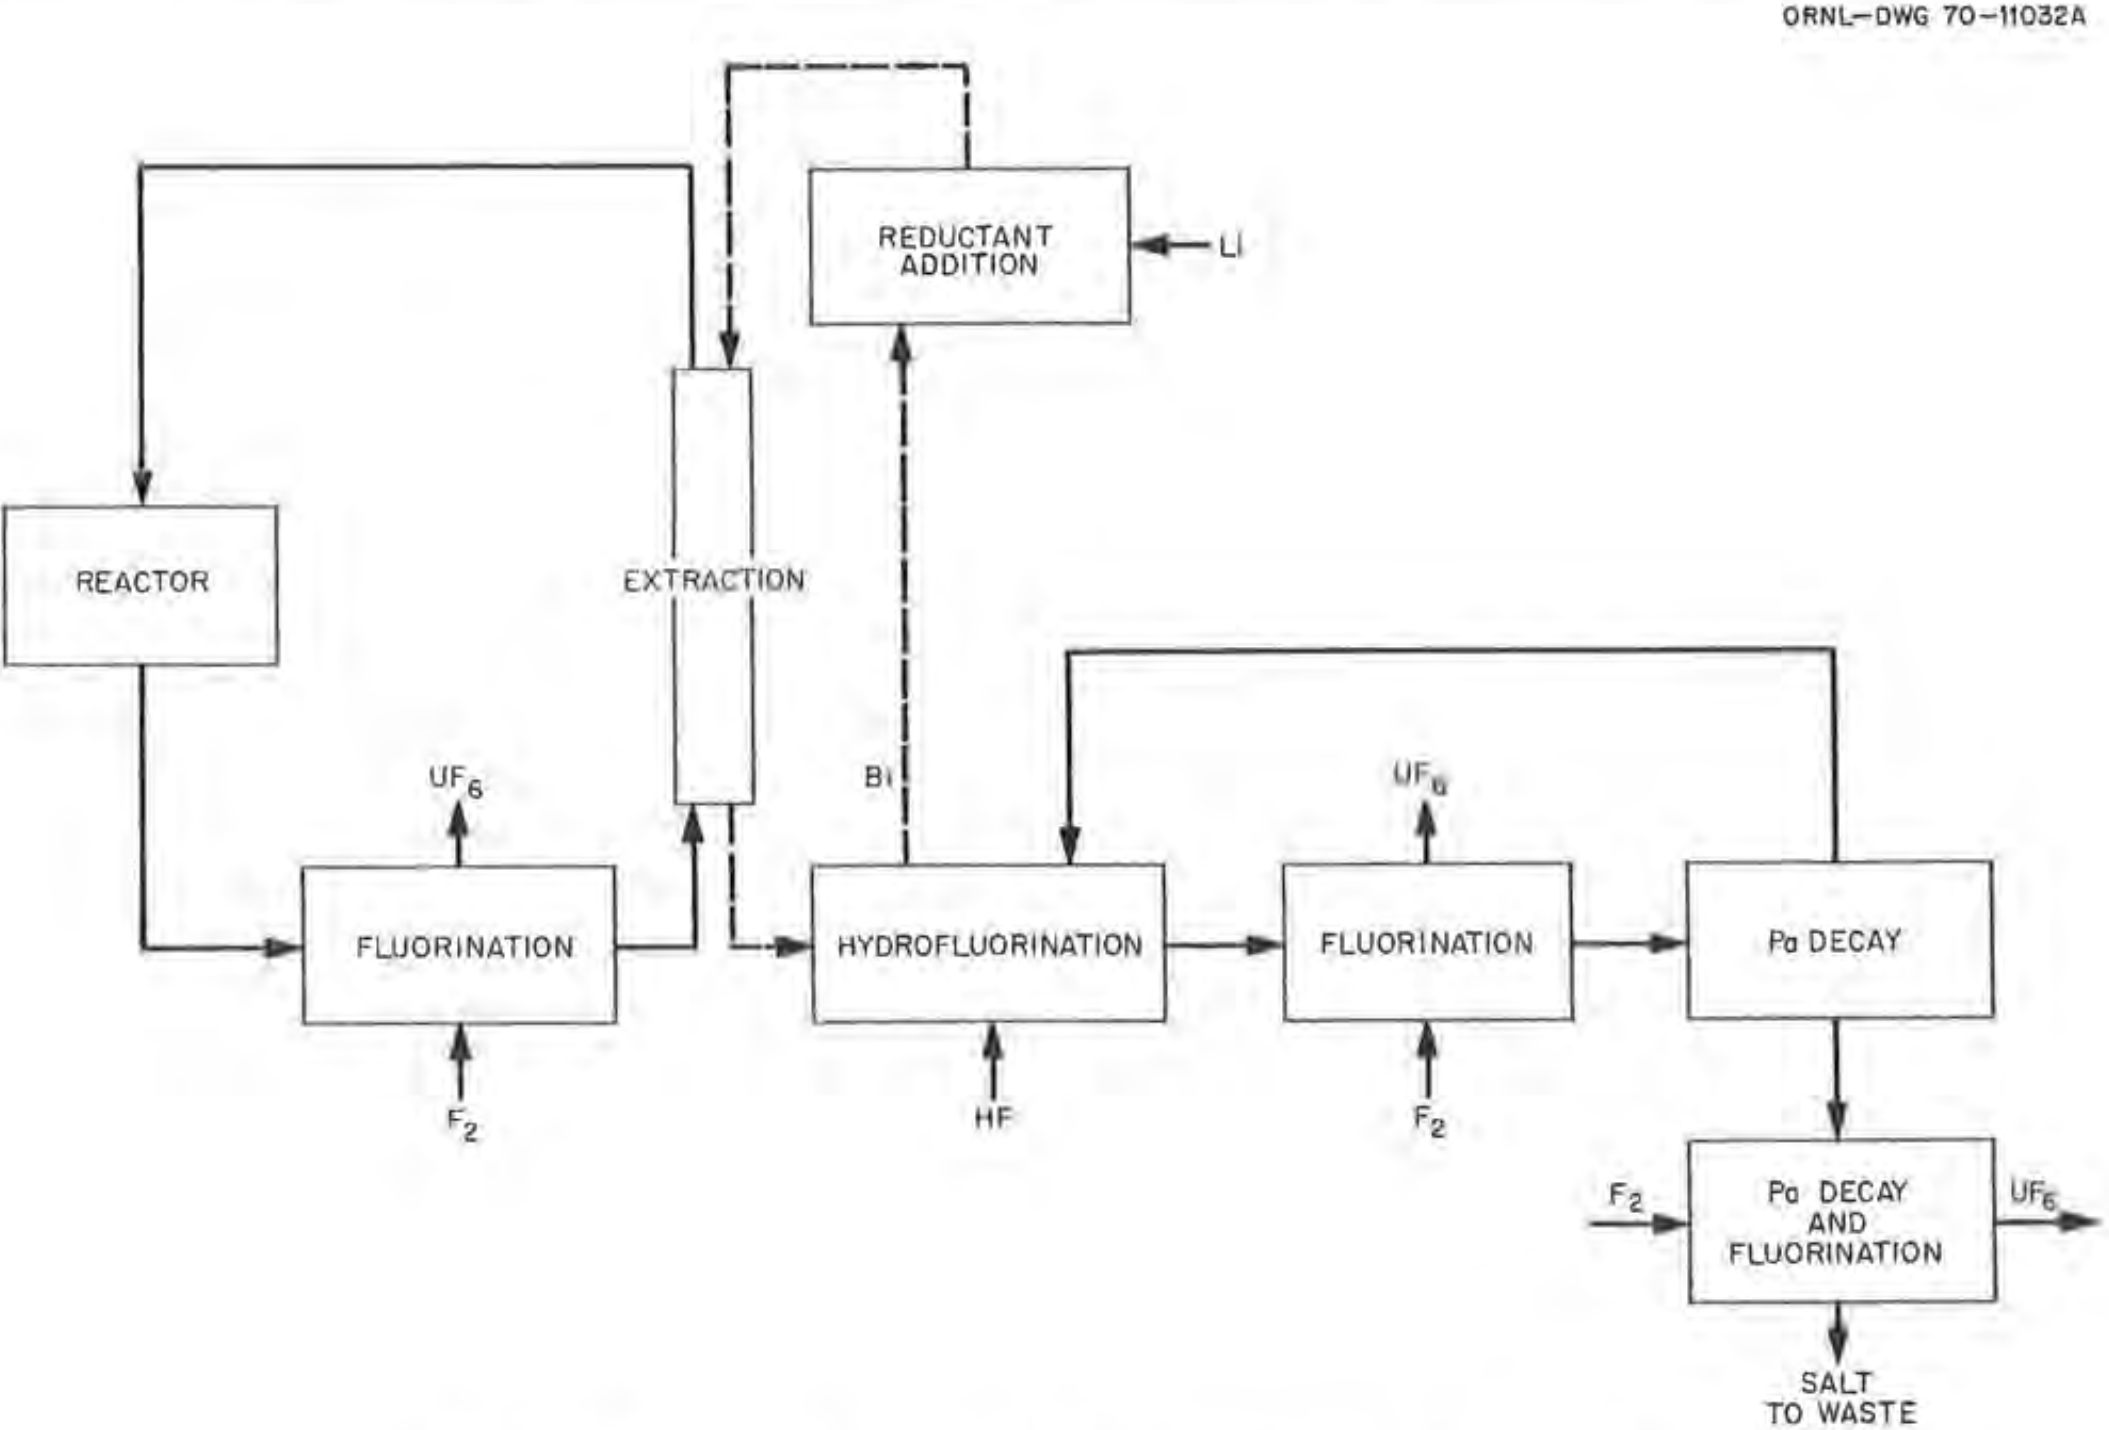
\includegraphics[width=0.8\textwidth]{figs/ch4/pa_removal_loop.png}
    \caption{\ce{^{233}Pa} removal loop. Reproduced from Figure 8.1 in \cite{robertson_conceptual_1971}}
    \label{fig:pa-removal}
\end{figure}

\paragraph{Rare-earth removal system}
The rare-earth removal system utilized the same metal transfer process used to
isolate protactinium from the fuel salt \cite{robertson_conceptual_1971}. This
system begins at the output of the extractor column for protactinium isolation.
It is a multistage extraction system:
\begin{enumerate}
    \item In the first extractor, the salt stream from the protactinium loop
    extractor column comes into contact with a bismuth stream containing 0.2 mol-\%
    lithium and 0.25 mol-\% thorium. The bismuth stream picks up a fraction of
    the rare earths and routes to the second extractor.
    \item In the second extractor, the bismuth stream containing rare earths is
    contacted with a \ce{LiCl} stream.  The \ce{LiCl} stream picks up a fraction
    of the rare earths (with trace amounts of thorium), and is routed to the
    fourth extractor. The bismuth stream is returned to the first extractor.
    \item In the fourth extractor, the \ce{LiCl} stream comes into contact with a
    circulating bismuth stream containing 5 mol-\% lithium. This bismuth stream
    removes trivalent rare earths from the \ce{LiCl} stream. The \ce{LiCl}
    stream is returned to the second extractor, however 2\% of this \ce{LiCl}
    stream is routed to the third extractor.
    \item In the third extractor, the \ce{LiCl} stream comes into contact with a
    circulating bismuth stream containing 50 mol-\% lithium. This bismuth stream
    removes divalent and alkaline rare earths from the \ce{LiCl} stream. The
    \ce{LiCl} stream is rerouted back to the second extractor.
\end{enumerate}

Figure \ref{fig:metal-removal} shows a block diagram of this loop. 

\begin{figure}[htpb]
    \centering
    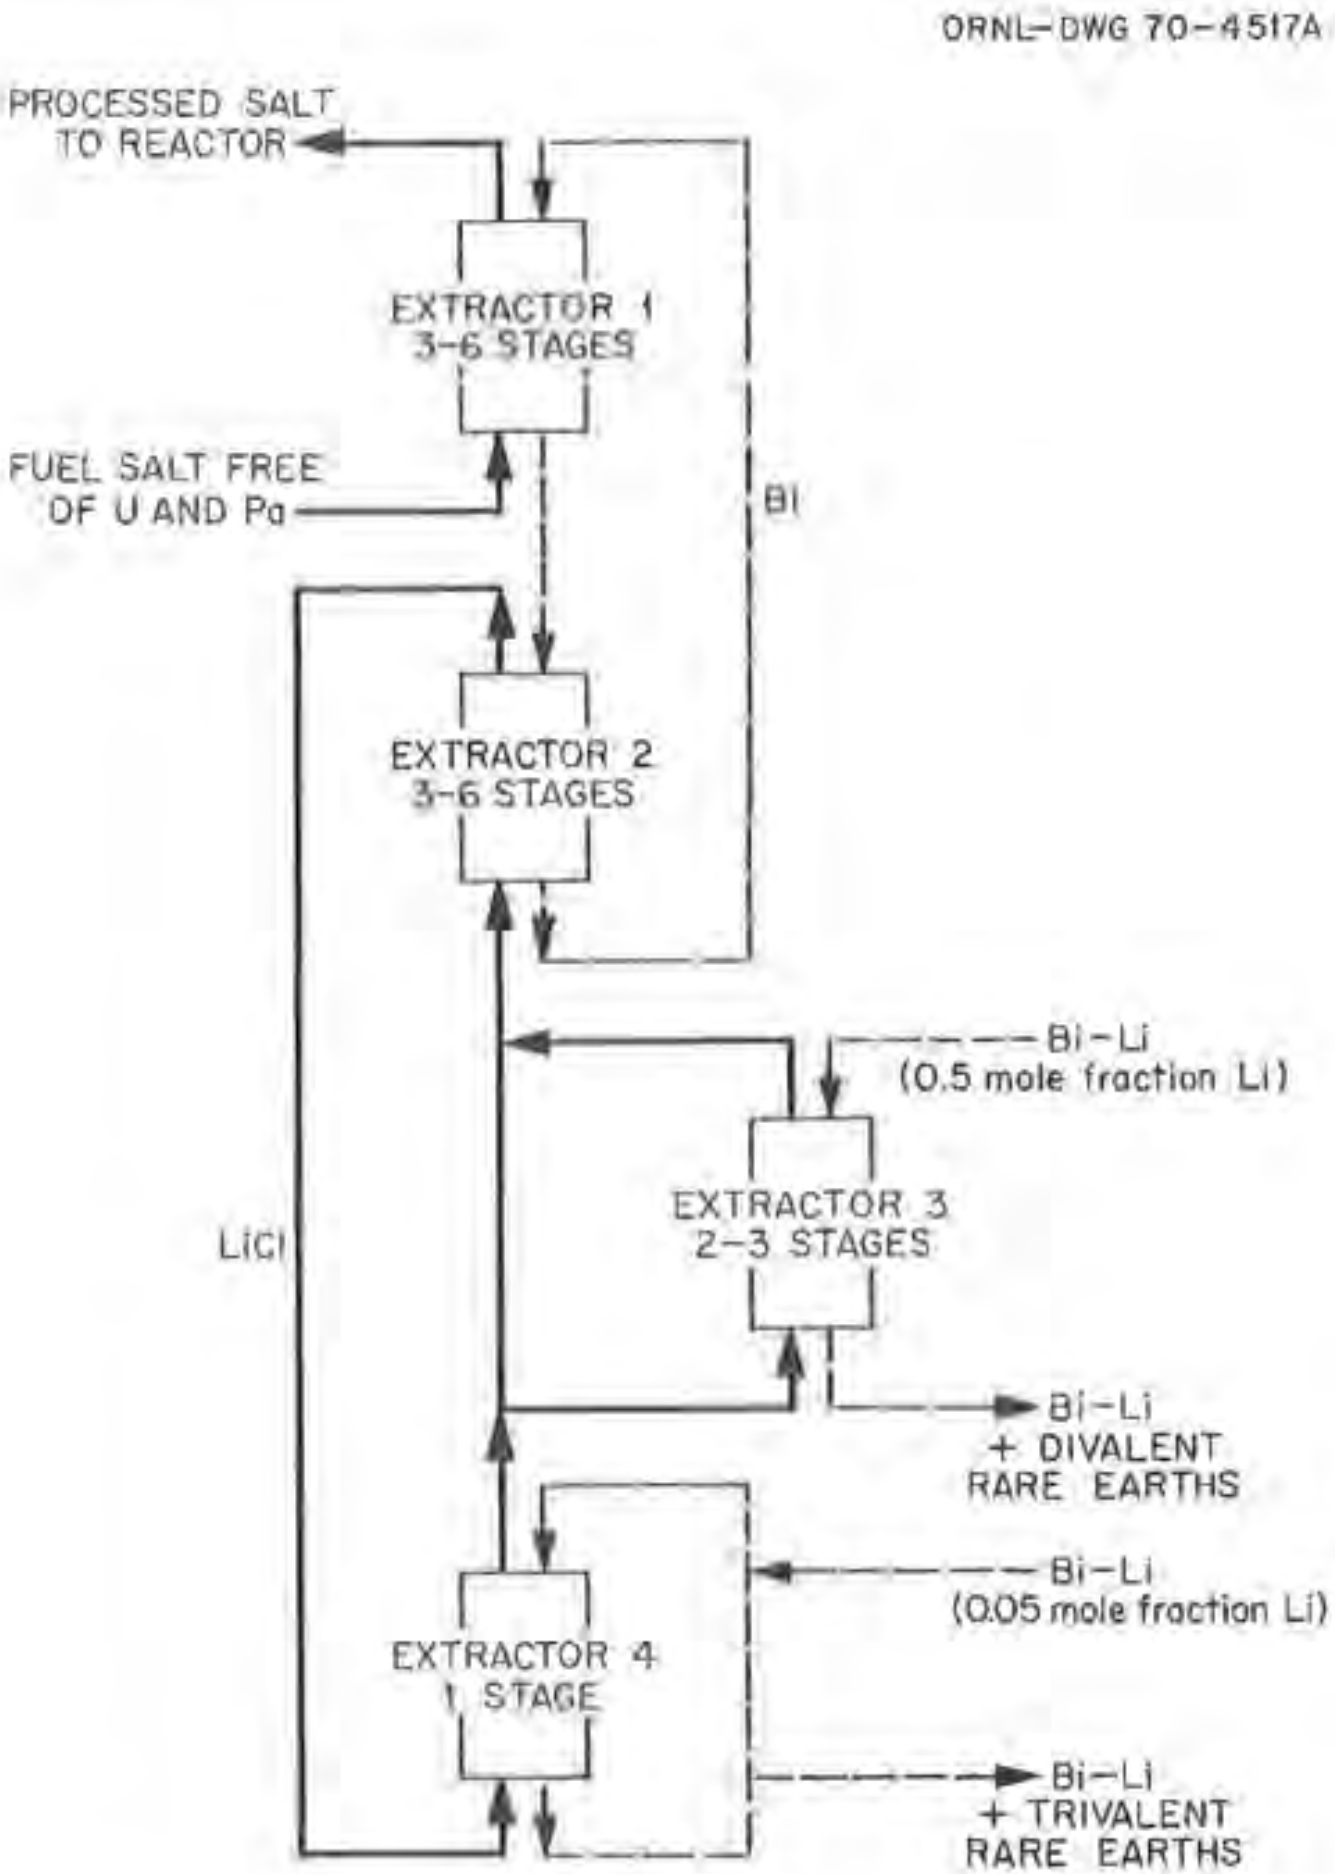
\includegraphics[width=0.3\textwidth]{figs/ch4/metal_removal_loop.png}
    \caption{Metal removal loop. Reproduced from Figure 8.2 in \cite{robertson_conceptual_1971}}
    \label{fig:metal-removal}
\end{figure}

\paragraph{Nickel-mesh filter}
Insoluble impurities in the processed salt needs to be removed at two locations:
before the salt stream is sent to reductive extraction system
\cite{lindauer_design_1969}, and before the processed salt stream coming
from the reductive extraction system returns to the
reactor \cite{robertson_conceptual_1971}. There are two filters, both
consisting of a nickel mesh \cite{robertson_conceptual_1971}.
The first filter removes insoluble impurities from transmutation and corrosion in the core, heat exchanger, and
other systems. The second filter removes  bismuth entrained or dissolved in the
fuel salt as a side effect from processing, and any additional insoluble
impurities such as \ce{FeF_2} and \ce{NiF_2}. 

\subsection{Reprocessing system model}
\label{sub:reprocessing-system-model}
As described in Section \ref{sub:feeds-separations}, SaltProc relies on extraction efficiencies to model chemical removal of target elements from the fuel salt.  Unfortunately, Robertson et al. (1971) 
\cite{robertson_conceptual_1971} provide no such values, and a literature review
to find such values is outside the scope of this thesis. What Robertson does
give us are the cycle times for elements in the fuel salt.

\begin{table}[htpb] 
    \centering 
    \caption{Reprocessing system cycle times. A combination of tables 3.7B in \cite{robertson_conceptual_1971}, Table 3 in \cite{carter_design_1972}, and Table 25.1 in \cite{rosenthal_molten-salt_1970}}
    \label{tab:msbr-cycle-times}
    \begin{tabularx}{500pt}{|X|X|X|X|X|} 
        \hline
        Processing group & Target component(s) & Cycle time for processing & Primary mechanism of removal from salt & Secondary mechanism of removal from salt\\
        \hline
        Protactinium & \ce{^{233}Pa} & 3 days & Reductive extraction with \ce{Bi-Li} in \ce{Pa} extraction column followed by isolation in \ce{Pa} decay salt & None \\
        \hline
        Rare earths & Trivalent: \ce{Y}, \ce{La}, \ce{Ce}, \ce{Pr}, \ce{Nd}, \ce{Pm}, \ce{Gd}, Divalent: \ce{Sm}, \ce{Eu} & 50 days (500 for \ce{Eu}) & Reductive extraction with \ce{Bi-Li} in \ce{Pa} extraction column followed by isolation in \ce{Pa} decay salt & Reduction to metallic particulates by \ce{H_2} in reduction column followed by filtration\\
        \hline 
        Noble metals & \ce{Se}, \ce{Nb}, \ce{Mo}, \ce{Tc}, \ce{Ru}, \ce{Rh}, \ce{Pd}, \ce{Ag}, \ce{Sb}, \ce{Te} & 20 sec & Plating out on surfaces in reactor vessel and heat exchangers & \ce{Nb}, \ce{Mo}, \ce{Tc}, \ce{Ru}, \ce{Rh},\ce{Sb}, and \ce{Te} have volatile fluorides and are removed in fluorinators; \ce{Pd}, \ce{Ag } reduced by \ce{Bi-Li} alloy in reductive extraction.\\
        \hline
        Seminoble metals & \ce{Zr}, \ce{Cd}, \ce{In}, \ce{Sn} & 200 days & Plating out on surfaces in ractor vessel and heat exchangers & Reductive extraction with \ce{Bi-Li} in \ce{Pa} extraction column followed by isolation in \ce{Pa} decay salt \\
        \hline
        Gases & \ce{Kr}, \ce{Xe} & 20 sec & Sparged from salt with \ce{He} gas in primary loop & Purged in fluorniators due to sparging action of \ce{F_2} and \ce{H_2}\\
        \hline
        Halogens & \ce{Br}, \ce{I} & 60 days & Volatilization in primary fluorinator & None \\
        \hline
        Carrier salt & \ce{Th}, \ce{Li}, \ce{Be}, \ce{F} & 3435 days & Fuel salt discard to remove excess \ce{Li} added in reductive extraction process. & None \\
        \hline
        Alkaline earths; alkali metals & \ce{Sr}, \ce{Ba}; \ce{Rb}, \ce{Cs} & 3435 days & Fuel salt discard & None \\
        \hline
    \end{tabularx}
\end{table}

Rykhlevskii previously used 100\% extraction efficiency with 3-day depletion
steps \cite{rykhlevskii_modeling_2019} using SaltProc v0.1.0. As mentioned in
Section \ref{sec:saltproc-history}, this version of SaltProc required the user
to hardcode in the cycle times. The program would then extract the target
elements from the fuel once a full cycle time had passed. In SaltProc v0.2.0 and
onward, this cycle time capability was removed in favor of user-defined
extraction efficiencies. This means we are unable to completely reproduce the
results in Ryklevskii et al. (2019)\cite{rykhlevskii_modeling_2019} as all extractions now happen after
every depletion step, rather than only after the hardcoded cycle times.
To get around this, we can construct proxy extraction efficiencies based on the
cycle times that will remove a large majority of the material after the
designated amount of time has passed.

Assuming we are running a simulation with constant-length depletion steps, let
$l_{d}$ be the length of a depletion step, and let $c_{x}$ be the cycle time for
element $X$. Ignoring the addition of element $X$ to the material via
transmutation or feeds, we can define the extraction efficiency $\epsilon_{x}$
to be:

\begin{equation}
    \label{eq:extraction-efficiency}
    \epsilon_{x} = 1 - \delta^{\frac{l_{d}}{c_{x}}}
\end{equation}

where $\delta$ is a threshold for the mass fraction remaining of the original
amount of element X\footnote{See Appendix \ref{appex:extraction-efficiency} for
the derivation of this equation.}. We will use $\delta = 1\cdot 10^{-16}$. Note
that our equation does not account for the addition of material.

The process graph is a simplified version of the processing system described 
above. There are only three components: the gas separator, the nickel filter and
the reductive extractor. Figure \ref{fig:process-graph} displays the process
graph. This simple configuration is designed to match results from Rykhlevskii
and Park et al. (2015) \cite{park_whole_2015} by processing 100\% of the salt
flow. Note the presence of a \verb.thorium_feed. feed process. This
process replaces the lost mass via reprocessing with an equal mass of fuel salt
of identical composition to the initial fuel salt, but with all \ce{^{233}U}
replaced by \ce{^{232}Th}. This ensures we have a relatively constant level of
\ce{^{232}Th} in the reactor. This process graph differs from Ryklevskii's
in \cite{rykhlevskii_fuel_2020}, as seen in Figure \ref{fig:rykhlevskii-process-graph}.
I did not use Ryklevksii's process graph as it incorporates more complicated
physics-based modeling of gas sparging that I felt did not fit in the scope
of this thesis.

\begin{figure}[htpb]
    \centering
    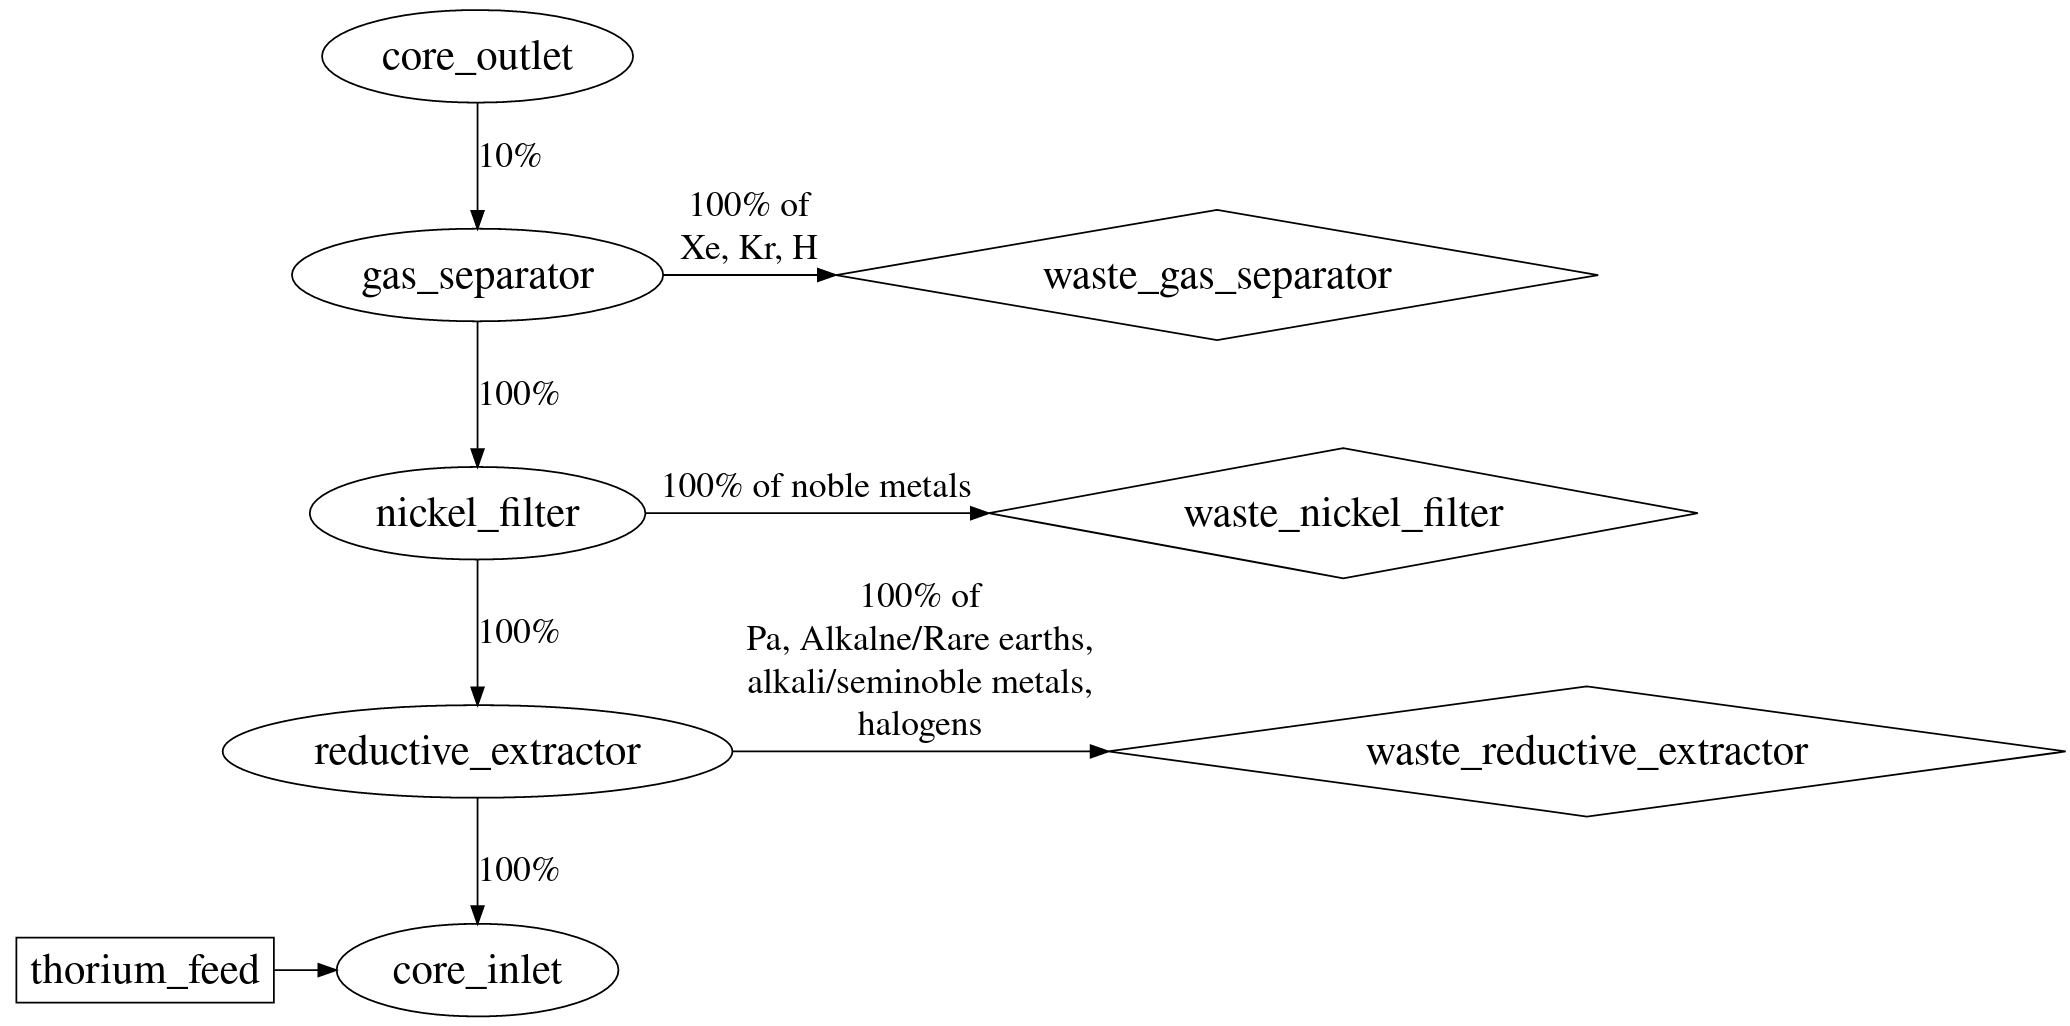
\includegraphics[width=0.8\textwidth]{figs/ch4/process_graph.png}
    \caption{Process graph for model salt reprocessing system}
    \label{fig:process-graph}
\end{figure}

\begin{figure}[htpb]
    \centering
    \includegraphics[width=0.8\textwidth]{figs/ch4/rykhlevskii-process-graph.png}
    \caption{Process graph for salt reprocessing system used in \cite{rykhlevskii_fuel_2020}}
    \label{fig:rykhlevskii-process-graph}
\end{figure}

Table \ref{tab:msbr-cycle-times} lists element groups and their extraction
efficiencies for depletion step length of 3 days. Note the inclusion of hydrogen
removal in the gas separator process. I added this to remove any tritium from the fuel. A 3 day depletion step size is
commonly chosen for modeling efforts of the \Gls{msbr} \cite{rykhlevskii_modeling_2019}
\cite{park_whole_2015}, as this corresponds to the the cycle time for \ce{^{233}Pa}
(which decays into \ce{^{233}U}), and strikes a good balance between capturing the
effect of short-lived fission products, and having a reasonable amount of depletions steps.
For this reason, I also use a 3 day depletion step size.
\begin{table}[htpb] 
    \centering 
    \caption{Extraction efficiencies using cycle times in Table \ref{tab:msbr-cycle-times} and Equation \ref{eq:extraction-efficiency}}
    \label{tab:msbr-cycle-times}
    \begin{tabularx}{400pt}{|X|X|X|X|X|} 
        \hline
        Processing group & Target component(s) & Cycle time for processing & Processing component & Extraction efficiency\\
        \hline
        Protactinium & \ce{^{233}Pa} & 3 days & reductive extractor & 1\\
        \hline
        Rare earths & Trivalent: \ce{Y}, \ce{La}, \ce{Ce}, \ce{Pr}, \ce{Nd}, \ce{Pm}, \ce{Gd}, Divalent: \ce{Sm}, \ce{Eu} & 50 days (500 for \ce{Eu}) & reductive extractor & 0.8904 (0.2 for \ce{Eu})\\
        \hline 
        Noble metals & \ce{Se}, \ce{Nb}, \ce{Mo}, \ce{Tc}, \ce{Ru}, \ce{Rh}, \ce{Pd}, \ce{Ag}, \ce{Sb}, \ce{Te} & 20 sec & nickel filter & 1\\
        \hline
        Seminoble metals & \ce{Zr}, \ce{Cd}, \ce{In}, \ce{Sn} & 200 days & reductive extractor & 0.425\\
        \hline
        Gases & \ce{Kr}, \ce{Xe}, \ce{H} & 20 sec & gas separator & 1\\
        \hline
        Halogens & \ce{Br}, \ce{I} & 60 days & reductive extractor & 0.842\\
        \hline
        Alkaline earths; alkali metals & \ce{Sr}, \ce{Ba}; \ce{Rb}, \ce{Cs} & 3435 days & reductive extractor & 0.032 \\
        \hline
    \end{tabularx}
\end{table}

\section{Cross Section Data}
\label{sec:xs-data}
Ryklevskii used the JEFF 3.1.2 cross section library in the initial evaluation
of the \Gls{msbr} CSG model. I was unable to convert the JEFF 3.1.2
library to \OpenMC's HDF5 format, so I am instead using the ENDF/B-VII.1 cross
section library. Section \ref{sub:results-xs-data} provides a more in-depth
discussion of the cross section data used.

\section{Differences between the \OpenMC and \SerpentTWO models}
The only differences between the \OpenMC and \SerpentTWO CSG models are in the
construction of the geometry. The \OpenMC model is constructed programmatically
using the OpenMC Python API, whereas the \SerpentTWO model is written entirely
in an input file. I encourage interested readers to compare the files stored at
\url{github.com/arfc/2022-yardasol-ms/tree/model/} under \verb.openmc/. and
\verb.serpent/.

\section{Eigenvalue and source distribution convergence}
Both \SerpentTWO and \OpenMC are monte-carlo codes that rely on the Method of
Successive Generations to perform eigenvalue calculations. A complete
description of this method is outside the scope of this thesis, but it requires
that the source distribution of particles and our $k_{\text{eff}}$ values
be converged before counting reaction tallies. In practice, the source
distribution converges much slower than $k_{\text{eff}}$, so we must pick our
a number of inactive batches that enables the source distribution to
converge. We do this experimentally by plotting the Shannon entropy
versus the batch number. The source distribution is converged when the 
Shannon entropy levels out.\footnote{\OpenMC discusses how it calculates Shannon entropy
on this page: \url{https://docs.openmc.org/en/stable/methods/eigenvalue.html\#diagnosing-convergence-with-shannon-entropy},
and I assume \SerpentTWO uses a similar method.}

I did not perform a detailed convergence study, and by trial-and error found
that using around 80 inactive batches ensures our source distributions for both
the \OpenMC and \SerpentTWO models are well converged, as seen in Figures
\ref{fig:msbr-source-convergence-openmc} and \ref{fig:msbr-source-convergence-serpent},
respectively.\footnote{I do not know why the Shannon entropy values between the
\SerpentTWO and \OpenMC results are so different.}

\begin{figure}[htpb]
    \centering
    \subfloat[][]{
        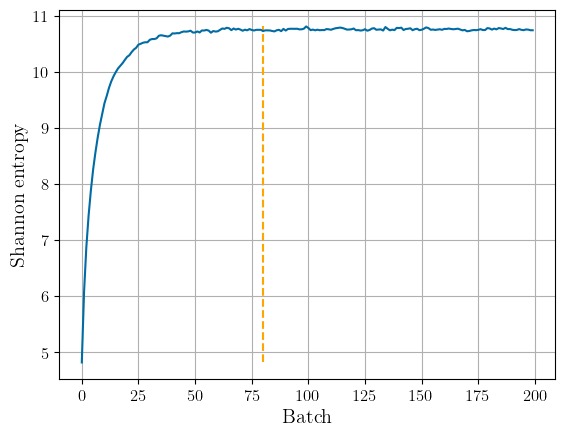
\includegraphics[width=0.5\linewidth]{figs/ch4/openmc_source_convergence.png}
        \label{fig:msbr-source-convergence-openmc}
    }
    \subfloat[][]{
        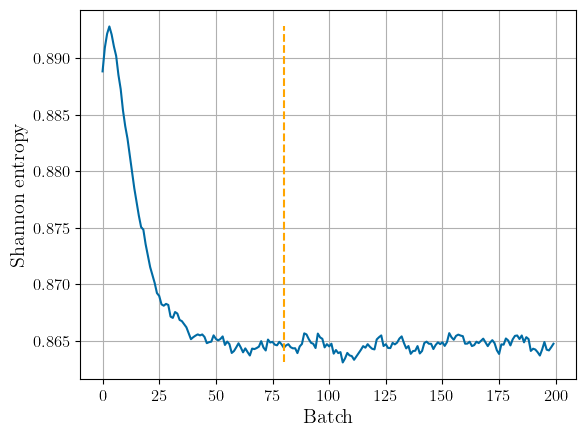
\includegraphics[width=0.5\linewidth]{figs/ch4/serpent_source_convergence.png}
        \label{fig:msbr-source-convergence-serpent}
    }
    \caption[MSBR source convergence]{MSBR source convergence
        for both \OpenMC and \SerpentTWO:
        \subref{fig:msbr-source-convergence-openmc} \OpenMC;
        \subref{fig:msbr-source-convergence-serpent} \SerpentTWO;
        both simulations performed using 80 inactive, 120 active batches,
        100k particles per batch
    }
    \label{fig:msbr-source-convergence}
\end{figure}

For completeness, Figure \ref{fig:msbr-keff-convergence} shows the convergence
of $k_{\text{eff}}$ vs. Batch number for \OpenMC and \SerpentTWO. Note that
$k_{\text{eff}}$'s convergence is better in the \SerpentTWO simulation
than in the \OpenMC simulation. The range of converged $k_{\text{eff}}$ for
the \SerpentTWO simulation is roughly 1000pcm, whereas the range for
the same quantity in the \OpenMC simulation is roughly 2000pcm. This
difference may be a contributing factor to differences in reported $k_{\text{eff}}$
values between the two codes even when the model, data, and methods are
identical.

\begin{figure}[htpb]
    \centering
    \subfloat[][]{
        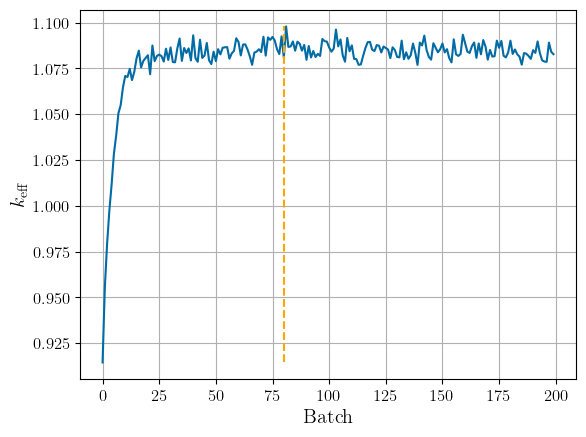
\includegraphics[width=0.5\linewidth]{figs/ch4/openmc_keff_convergence.png}
        \label{fig:msbr-keff-convergence-openmc}
    }
    \subfloat[][]{
        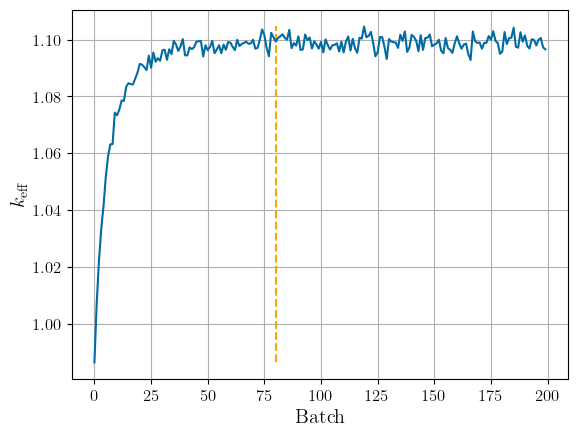
\includegraphics[width=0.5\linewidth]{figs/ch4/serpent_keff_convergence.png}
        \label{fig:msbr-keff-convergence-serpent}
    }
    \caption[MSBR $k_\text{eff}$ convergence]{MSBR $k_\text{eff}$ convergence
        for both \OpenMC and \SerpentTWO:
        \subref{fig:msbr-keff-convergence-openmc} \OpenMC;
        \subref{fig:msbr-keff-convergence-serpent} \SerpentTWO;
        both simulations performed using 80 inactive, 120 active batches,
        100k particles per batch
    }
    \label{fig:msbr-keff-convergence}
\end{figure}
